% !TeX spellcheck = en_GB
\chapter{Anyon chains}
\label{sec:anyons}

In this chapter, we introduce the concept of \emph{anyon chains}, which is the most important tool in our search for a Conformal Field Theory (CFT) that corresponds to the Haagerup subfactor. Anyons are exotic quasiparticles that can occur in two-dimensional systems, whose statistical behaviour is much less restricted than those of bosons and fermions. Mathematically, they are described by Unitary Modular Tensor Categories (UMTC). 

Anyons are highly interesting for several reasons: Firstly, they can be employed to perform fault-tolerant quantum computation in the context of \emph{topological quantum computation} \cite{Nayak2008,Pachos2009,Wang2010,kitaev_anyons_2006}. Since most of the quasiparticle details are not relevant for the description of anyons (in fact, only topological properties matter), computations using these particles are resistant against errors in the control of the quasiparticles. For instance, in \cite{Kitaev2003} Kitaev proposed a topological quantum error correcting code, the \emph{toric code}, defined on a two-dimensional spin lattice with periodic boundary conditions. In this model, the information is encoded in the ground state space of the Hamiltonian such that errors appear as excitations that can be detected due to an energy gap above the ground states. Another interesting example are computational models coming from the Fibonacci category, since they allow for \emph{universal} quantum computation: any quantum circuit acting on $n$ qubits can be realised using $4n$ physical Fibonacci anyons (see \cite{Freedman2002} and \cite{Preskill2004}).

Anyonic statistics can be observed in the fractional quantum Hall effect \cite{Arovas1984,Halperin1984,Jeon2003,CAS13}. However, it has taken a long time for non-abelian anyons (see below for an explanation of the term \emph{non-abelian}) to actually be observed in an experiment. While there was some evidence for non-abelian anyons reported in \cite{Willett2013}, it has been pointed out in \cite{Keyserlingk2015} that the observed phenomena might come from certain Coulomb effects instead of properties of non-abelian anyons. Recent works show new evidence for the existence of anyonic quasiparticles: While in \cite{Bartolomei2020} anyonic statistics were indirectly observed via noise correlation measurements, the authors of \cite{Nakamura2020} have been able to directly observe these statistics.

Apart from being a promising candidate for topological quantum computation, anyons are an important tool in our search for a Haagerup CFT: As it was investigated in \cite{feiguin_interacting_2007} and \cite{Finch2014}, among others, they are connected to CFTs via a one-dimensional chain constructed from the underlying UMTC. This can be thought of as an analogue to spin chains\index{spin chain}: Consider a chain of spin-$\frac{1}{2}$ particles. Two neighbouring spin-$\frac{1}{2}$ degrees of freedom will either combine to a spin-$0$ state, i.e., a singlet state $|\mathbf{0}\rangle$, or a spin-$1$ state, which is a triplet state $|\mathbf{1}\rangle$. Hence, we can picture this chain with spin-$\frac{1}{2}$ particles on the lattice sites and singlet and triplet states living on the bonds of this chain:
	\begin{figure}[H]
		\centering
		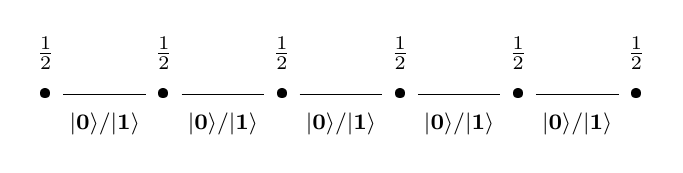
\begin{tikzpicture}[scale=1.5]
			\node at (0,0) {\textbullet};
			\node at (1,0) {\textbullet};
			\node at (2,0) {\textbullet};
			\node at (3,0) {\textbullet};
			\node at (4,0) {\textbullet};
			\node at (5,0) {\textbullet};
			\draw (0.15,0) -- (0.85,0);
			\draw (1.15,0) -- (1.85,0);
			\draw (2.15,0) -- (2.85,0);
			\draw (3.15,0) -- (3.85,0);
			\draw (4.15,0) -- (4.85,0);
			\node at (0,+0.35) {$\frac{1}{2}$};
			\node at (1,+0.35) {$\frac{1}{2}$};
			\node at (2,+0.35) {$\frac{1}{2}$};
			\node at (3,+0.35) {$\frac{1}{2}$};
			\node at (4,+0.35) {$\frac{1}{2}$};
			\node at (5,+0.35) {$\frac{1}{2}$};
			\node at (0.5,-0.25) {\footnotesize $|\mathbf{0}\rangle/|\mathbf{1}\rangle$};
			\node at (1.5,-0.25) {\footnotesize $|\mathbf{0}\rangle/|\mathbf{1}\rangle$};
			\node at (2.5,-0.25) {\footnotesize $|\mathbf{0}\rangle/|\mathbf{1}\rangle$};
			\node at (3.5,-0.25) {\footnotesize $|\mathbf{0}\rangle/|\mathbf{1}\rangle$};
			\node at (4.5,-0.25) {\footnotesize $|\mathbf{0}\rangle/|\mathbf{1}\rangle$};
		\end{tikzpicture}
	\end{figure}

Our goal is to find an analogous way of constructing an anyon chain starting from a UMTC. We begin this chapter by describing anyonic statistics and the underlying algebraic theory in detail, thereby focussing on how the physical properties of anyons arise from the underlying structure of the UMTC. Then we present the constriction of chain models for anyons and explain how a numerical investigation of the ground state yields information about the corresponding conformal field theory. Here, we make use of tensor network methods (more precisely, matrix product states) to be able to efficiently study the model numerically. Finally, we apply these methods to the Haagerup fusion category $\Hd$ in order to investigate whether there is a conformal field theory corresponding to the Haagerup subfactor.


\section{Anyonic statistics}

\index{anyons}
For a moment, we will leave the mathematical concepts we have discussed in the previous chapters and focus on some physical phenomena. As quantum mechanics tells us, indistinguishable particles in three spatial dimensions come in two species: bosons and fermions. Consider now a system of two identical particles. One particle circulates around the other particle via the path $C_1$ as shown in \cref{fig:particleloop}\textbf{(a)}. In three spatial dimensions, the path $C_1$ can be continuously deformed into the path $C_2$ simply by lifting the loop above the second particle. We are only interested in topological properties, hence the particular geometry of the path does not have any effect. $C_2$ can further be deformed into the trivial path (which we simply denote $0$), which is the path that leaves the particle at its original position at all times. 

In two spatial dimensions, the situation is a little different. As shown in \cref{fig:particleloop}\textbf{(b)}, it is now impossible to lift the path $C_2$ above the second particle to continuously deform it into the path $C_1$. We would instead have to cut the path, pass it over the particle and glue it together again, but this would change the topological properties of the path. Hence, in two dimensions, the paths $C_2$ and $C_1$ are topologically different. Despite this difference, note that $C_2$ can still be deformed to the trivial path. 

	\begin{figure}[t]
		\begin{tikzpicture}[scale=1]
			\node at (-0.5,2.1) {\textbf{(a)}};
			\begin{scope}[scale=0.8]
				\draw[->,>=stealth] (0,0) -- (1,0);
				\draw[->,>=stealth] (0,0) -- (0,1);
				\draw[->,>=stealth] (0,0) -- (225:0.7071);
			\end{scope}
			\draw[->-] (0.75,1.25) arc (180:-180:0.75cm and 0.4cm);
			\draw[->-] (0.75,1.25) arc (180:-180:1.5cm and 0.6cm);
			\shade[ball color = LinkColor!90, opacity = 1] (0.75,1.25) circle (0.25cm);
			\shade[ball color = LinkColor!90, opacity = 1] (3,1.25) circle (0.25cm);
			\node at (4,1.5) {$C_1$};
			\node at (2.45,1.5) {$C_2$};
		\end{tikzpicture}\hspace{15pt}
		\begin{tikzpicture}[scale=1]
			\node at (-0.75,2.25) {\textbf{(b)}};
			\draw[fill=LightGray,LightGray] (-0.75,-0.25) -- (4,-0.25) -- (5.5,2.25) -- (0.75,2.25) -- cycle;
			\begin{scope}[scale=0.8,xshift=-0.45cm,yshift=0cm]
			\draw[->,>=stealth] (0,0) -- (1,0);
			\draw[->,>=stealth] (0,0) -- (58:0.7071);
			\end{scope}
			\draw[->-] (0.75,1.25) arc (180:-180:0.75cm and 0.4cm);
			\draw[->-] (0.75,1.25) arc (180:-180:1.5cm and 0.6cm);
			\draw[fill=LinkColor!90,LinkColor!90] (0.75,1.25) ellipse (0.25cm and 0.18cm);
			\draw[fill=LinkColor!90,LinkColor!90] (3,1.25) ellipse (0.25cm and 0.18cm);
			\node at (4,1.5) {$C_1$};
			\node at (2.45,1.5) {$C_2$};
		\end{tikzpicture}
	\caption{\small \label{fig:particleloop}\textbf{Topological differences between three- and two-dimensional particle circulation.} \textbf{(a)} A particle spans a loop around another particle (path $C_1$). In three dimensions, it is always possible to continuously deform the path $C_1$ into the path $C_2$, which is equivalent to a trivial path. \textbf{(b)} In two dimensions, the paths are topologically distinct: $C_1$ cannot be continuously deformed into $C_2$.}
	\end{figure}

What does this observation tell us about the statistics of these particles? In the three-dimensional case, the wave function $\Psi$ of the system after the circulation $C_1$ has to be exactly the same as the original wave function:
	\begin{equation}
	\label{eq:waveequiv}
		\Psi(C_1)=\Psi(C_2)=\Psi(0).
	\end{equation}
	
Furthermore, note that the circulation of one particle around another is equivalent to performing two exchanges of these particles (plus a spatial translation which is irrelevant because we are only interested in topological properties here), see \cref{fig:particleexchange}. Hence, the single exchange of two particles can yield a phase factor $e^{i\varphi}$ which has to square to one to fulfil \cref{eq:waveequiv}. This has exactly two possible solutions, $\varphi_b=0$ and $\varphi_f=\pi$, which corresponds to the bosonic\index{boson} and fermionic\index{fermion} statistics, respectively.

	\begin{figure}[t]
		\begin{tikzpicture}[scale=1.2]
			\begin{scope}[scale=0.7,xshift=0cm,yshift=0.5cm]
			\draw[->,>=stealth] (0,0) -- (1,0);
			\draw[->,>=stealth] (0,0) -- (0,1);
			\draw[->,>=stealth] (0,0) -- (225:0.7071);
			\end{scope}
			\draw[-->--] (0.75,1.25) to [bend left=30] (3,1.25);
			\draw[-->--] (3,1.25) to [bend left=30] (0.75,1.25);
			\shade[ball color = LinkColor!90, opacity = 1] (0.75,1.25) circle (0.25cm);
			\shade[ball color = LinkColor!90, opacity = 1] (3,1.25) circle (0.25cm);
		\end{tikzpicture}
		\caption{\small \label{fig:particleexchange}\textbf{A single exchange of two particles.} Two successive exchanges of two particles are equivalent to circulating one particle around the other (plus a spatial translation).}
	\end{figure}

In the two-dimensional case the situation is different. Since the path $C_1$ cannot continuously be deformed into the trivial path, there are a variety of possible statistical evolutions. We can now assign an arbitrary phase factor to the evolution that corresponds to the path $C_1$ (or, equivalently, two successive exchanges of particles) or even a unitary matrix. In the case where we assign an arbitrary phase factor to the evolution, the particles are called \emph{abelian anyons}\index{abelian anyon}. The factor can take any value between the bosonic case $e^{i\varphi_b}=1$ and the fermionic case $e^{i\varphi_f}=-1$\footnote{The fact that these particles can have any statistics has led to the name \emph{anyon} \cite{Wilczek1982}.}. 

Beyond this, it is possible to have more complex statistics that are described by a higher-dimensional unitary matrix. Anyons that have this kind of statistics are called \emph{non-abelian}\index{non-abelian anyon}\footnote{This name is motivated by the fact that matrices do not, in general, commute, in contrast to factors.}. For this kind of evolution to emerge, the wave function that describes the system has to be within a degenerate subspace of states. The matrix evolution then transforms between different states in this subspace, thereby leaving the energy of the system unchanged. Note that the initial considerations we made require the different states in this subspace to be \emph{indistinguishable}. This means that there are no local measurements that can detect the exchange of these particles.

\section{Algebraic theory of anyons}
\label{sec:alganyons}

Mathematically, anyons are described by Unitary Modular Tensor Categories (UMTCs) which have been defined in \cref{sec:MTC}. However, in this chapter we will take a more physical point of view and focus on the \emph{data} we need to describe a system of anyons. We then connect this data with the adjectives that appear in the definition of a UMTC. \Cref{tab:MTCanyons} provides a dictionary between the notation used in the description of anyon chains (that mostly originates from physics) and the categorical terms.

\subsection*{Particle types and fusion rules.}
To describe a system of anyons we first have to specify what kind of particles we allow, i.e., a set
	\begin{equation}
		\mathcal{M}=\{\mathbf{1},a,b,c,\dots\}.
	\end{equation}
Here, $\mathbf{1}$ denotes the (unique) vacuum, while $a,b,c,\dots$ correspond to a \emph{finite} series of different particle types\footnote{In the following, we will use the terminologies \emph{particle} and \emph{anyon} interchangeably.}. In the language of UMTCs, this set of particle types corresponds to the isomorphism classes of simple objects of which there are only finitely many (see \cref{def:fusioncat}).

The fusion rules\index{fusion rule} of an anyon model describe what happens if we bring two anyons close together and treat them as one composite object, hence describing how they statistically behave together. These rules are given in the form
	\begin{equation}
	\label{eq:fusionrules}
		a\otimes b=\sum_c N_{ab}^c\ c,
	\end{equation}
where $a,b,c$ are anyon types and the sum runs over all possible types. Since there might several distinct ways to produce particle $c$ when fusing $a$ and $b$, we have an integer factor $N_{ab}^c$ which is usually referred to as \emph{fusion multiplicity}\index{multiplicities}. 

	\begin{defn}[Multiplicity-free]
		\index{multiplicity-free}
		A fusion rule is multiplicity-free if $N_{ab}^c\in\{0,1\}$ for any choice of particle types $a,b,c$.
	\end{defn}

\begin{table}[t]
	\begin{tabular}{c|c}
		Anyonic system & Unitary MTC\\ \hline\\[-8pt]
		anyon & simple object\\
		fusion & tensor product\\
		fusion rules & fusion rules\\
		antiparticle & dual object\\
		quantum dimension & object dimension\\
		particle exchange & braiding
		\vspace{10pt}
	\end{tabular}
	\caption{\small \label{tab:MTCanyons}Dictionary of terms relating anyonic systems to unitary modular tensor categories (UMTCs).}
\end{table}

The ordering of the particles $a$ and $b$ in the fusion rules \cref{eq:fusionrules} is not important: it holds that
	\begin{equation}
		a\otimes b=b\otimes a.
	\end{equation}	
Fusing a particle with the vacuum is always trivial:
	\begin{align}
		a\otimes\mathbf{1}&=a\\
		\mathbf{1}\otimes b&=b.
	\end{align}
This property can also be expressed as $N_{a\mathbf{1}}^c=\delta_{ac}$ and $N_{\mathbf{1}b}^c=\delta_{bc}$. Each particle type $a$ has a unique antiparticle type $a^*$ such that $N_{ab}^\mathbf{1}=\delta_{ba^*}$. Furthermore, it holds that $\mathbf{1}^*=\mathbf{1}$ and $\left(a^*\right)^*=a$. The fusion multiplicities obey the following relation (see \cite{Bond2007}):
	\begin{align}
		\sum_e N_{ab}^e N_{ec}^d&=\sum_f N_{af}^d N_{bc}^f.
	\end{align}

The fusion rules also tell us whether the anyon model is abelian or non-abelian: In the abelian case, the anyons only have one fusion channel, i.e., every fusion rule is of the form 
	\begin{equation}
	\label{eq:abelian}
		a\otimes b=c.
	\end{equation}
In the non-abelian case there can be multiple fusion outcomes, which corresponds to
	\begin{equation}
	\label{eq:nonabelian}
		\sum_c N_{ab}^c>1.
	\end{equation}

Another important quantity is the so-called \emph{quantum dimension}\index{quantum dimension} of a particle. For a particle $a$ it is defined via the $F$-symbols of the category, which have been introduced in \cref{sec:fusioncat}:
	\begin{equation}
	\label{eq:qdimF}
		d_a=\left|\left(F_a^{aa^* a}\right)_{\mathbf{1}\mathbf{1}}\right|^{-1}.
	\end{equation}
Since the anyon model is unitary, it follows that $d_a\ge 1$ with equality if and only if $a$ is abelian (i.e., fusion with any other particle has exactly one fusion channel as in \cref{eq:abelian}). The total quantum dimension\index{total quantum dimension} of the model is defined as
	\begin{equation}
		\mathcal{D}=\sqrt{\sum_a d_a^2}.
	\end{equation}

Regarding the relation of anyons and modular tensor categories, the fusion operation of anyons corresponds to the tensor product in a UMTC. We have already seen how fusion multiplicities naturally emerge in a fusion category in \cref{rem:multiplicities}. Furthermore, the quantum dimension of a particle is directly related to the dimension of an object in a UMTC as defined in \cref{def:ctdim}. This will become more clear when we introduce the graphical depiction of the quantum dimension in \cref{eq:qdimgraph}.

Recall that the goal of this chapter is to build a one-dimensional chain of anyons similar to how spin chains are constructed. These anyon chains are of the form 
	\begin{equation}
		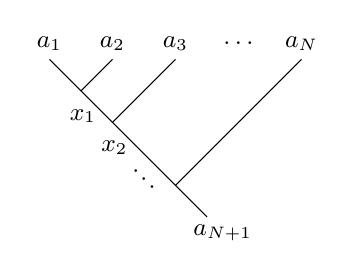
\begin{tikzpicture}[scale=0.8,baseline=(current bounding box.center)]
			\draw (0,0) -- (-2.5,2.5);
			\draw (-0.5,0.5) -- (1.5,2.5);
			\draw (-1.5,1.5) -- (-0.5,2.5);
			\draw (-2,2) -- (-1.5,2.5);
			\node at (0.25,-0.25) {\small $a_{N+1}$};
			\node at (-2.5,2.75) {\small $a_1$};
			\node at (-1.5,2.75) {\small $a_2$};
			\node at (-0.5,2.75) {\small $a_3$};
			\node at (1.5,2.75) {\small $a_N$};
			\node at (0.5,2.75) {\small $\dots$};
			\node at (-1.9,1.6) {\small $x_1\ $};
			\node at (-1.4,1.1) {\small $x_2\ $};
			\node at (-1,0.6) {\rotatebox{-45}{\small $\dots$}};
		\end{tikzpicture},
	\end{equation}
where every vertex corresponds to the splitting of one anyon into two. Hence, to be able to describe the Hilbert space and the dynamics of this system we need to translate the properties of the underlying fusion category to vector spaces and Hamiltonians. We begin by building vector spaces for the fusion and splitting of anyons.	

Given the fusion rules, we can assign vector spaces to fusion processes\index{fusion space}. For instance, consider two particles $a$ and $b$ that fuse to a particle $c$ with $N_{ab}^c=1$. This implies that there is exactly one way to fuse the particles $a$ and $b$ to $c$. Hence, the vector space that corresponds to this fusion process has to be one-dimensional. We will denote the corresponding fusion space $V_{ab}^c$ and vectors in this space are of the form
	\begin{equation}
		\begin{tikzpicture}[scale=0.5,baseline=(current bounding box.center)]
			\draw (0,0) -- (0,-1);
			\draw (0,-1) -- (-1,-2);
			\draw (0,-1) -- (1,-2);
			\node at (0,0.4) {$c$};
			\node at (-1.1,-2.4) {$a$};
			\node at (1.1,-2.4) {$b$};
		\end{tikzpicture}
	\end{equation}

There is a dual space to $V_{ab}^c$, namely the \emph{splitting space}\index{splitting space} $V_c^{ab}$. Their relation is the following: If $\psi\in V_c^{ab}$ is a splitting vector, then $\psi^\dagger\in V_{ab}^c$ is the dual vector in the fusion space:
	\begin{equation}
		\begin{tikzpicture}[scale=0.5,baseline=(current bounding box.center),yscale=-1]
		\node at (-0.55,-0.65) {$\psi$};
		\draw (0,0) -- (0,-1);
		\draw (0,-1) -- (-1,-2);
		\draw (0,-1) -- (1,-2);
		\node at (0,0.4) {$c$};
		\node at (-1.1,-2.4) {$a$};
		\node at (1.1,-2.4) {$b$};
		\end{tikzpicture},\hspace{20pt}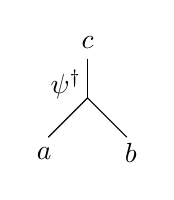
\begin{tikzpicture}[scale=0.5,baseline=(current bounding box.center)]
		\node at (-0.55,-0.65) {$\psi^\dagger$};
		\draw (0,0) -- (0,-1);
		\draw (0,-1) -- (-1,-2);
		\draw (0,-1) -- (1,-2);
		\node at (0,0.4) {$c$};
		\node at (-1.1,-2.4) {$a$};
		\node at (1.1,-2.4) {$b$};
		\end{tikzpicture}.
	\end{equation}
Since these vector spaces are the smallest possible fusion/splitting spaces, we will refer to them as the \emph{minimal} fusion/splitting spaces.

\begin{rem}
	If the fusion rules are multiplicity-free we can omit the Greek letter at the vertex of a fusion/splitting tree, since the space is one-dimensional in this case. In the following, we will usually consider the multiplicity-free case to avoid messy equations and diagrams, hence we will mostly use diagrams without Greek letters. However, we sometimes state an equation in both versions or make a comment to show what changes if we consider multiplicities. It should always be clear from the context which case we are considering since Greek letters occur if and only if the model is not multiplicity-free.
\end{rem}

\subsection*{The standard basis and $F$-matrices.}

When we fuse (or split) several anyons, there is a priori no preferred order of fusion (or splitting, respectively). We can choose several orders of fusion/splitting, which correspond to different choices of bases (we have already encountered this phenomenon when introducing $F$-symbols in \cref{ch:cats}). Therefore, we can choose a \emph{standard basis}\index{standard basis}, by which we mean the decomposition of a bigger fusion/splitting space into minimal fusion/splitting spaces. If we consider the splitting of a particle $u$ into $N$ particles $a_1,a_2,\dots,a_N$, we choose the corresponding standard basis to be of the form
	\begin{equation}
		V_u^{a_1,a_2,\dots,a_N}=\bigoplus_{e_2,e_3,\dots,e_{N-1}}V_{e_2}^{a_1a_2}\otimes V_{e_3}^{e_2a_3}\otimes V_{e_4}^{e_3a_4}\otimes\dots\otimes V_u^{e_{N-1}a_N}.
	\end{equation}
In terms of the previously introduced tree diagrams, the elements of this basis correspond to tree diagrams of the form
	\begin{equation}
		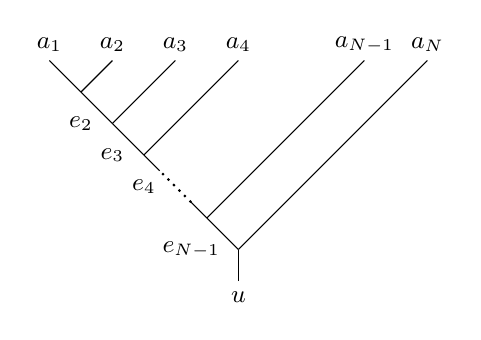
\begin{tikzpicture}[scale=0.8,baseline=(current bounding box.center)]
			\draw (0,0) -- (0,0.5);
			\draw (0,0.5) -- (-0.5,1);
			\draw (-0.5,1) -- (-0.75,1.25);
			\draw[dotted,thick] (-0.75,1.25) -- (-1.25,1.75);
			\draw (-1.25,1.75) -- (-1.5,2);
			\draw (-1.5,2) -- (-2,2.5);
			\draw (-2,2.5) -- (-2.5,3);
			\draw (-2.5,3) -- (-3,3.5);
			\draw (0,0.5) -- (3,3.5);
			\draw (-0.5,1) -- (2,3.5);
			\draw (-1.5,2) -- (0,3.5);
			\draw (-2,2.5) -- (-1,3.5);
			\draw (-2.5,3) -- (-2,3.5);
			\node at (0,-0.25) {\small $u$};
			\node at (-0.75,0.5) {\small $e_{N-1}$};
			\node at (-2,2) {\small $e_3$};
			\node at (-2.5,2.5) {\small $e_2$};
			\node at (-1.5,1.5) {\small $e_4$};
			\node at (-3,3.75) {\small $a_1$};
			\node at (-2,3.75) {\small $a_2$};
			\node at (-1,3.75) {\small $a_3$};
			\node at (0,3.75) {\small $a_4$};
			\node at (2,3.75) {\small $a_{N-1}$};
			\node at (3,3.75) {\small $a_N$};
		\end{tikzpicture}.
	\end{equation}
This can analogously be defined for the fusion basis. We can extend the definition of a standard basis to involve both fusion and splitting spaces. The most general form is a vector space $V_{a_1',a_2',\dots,a_M'}^{a_1,a_2,\dots,a_N}$, where $M$ particles $a_1',\dots,a_M'$ are transformed into $N$ particles $a_1,\dots,a_N$. This can be performed in two steps: First, fusing the $M$ ingoing particles into one and then splitting them into the $N$ outgoing particles. In terms of the standard basis, the corresponding tree diagrams are of the form
	\begin{equation}
		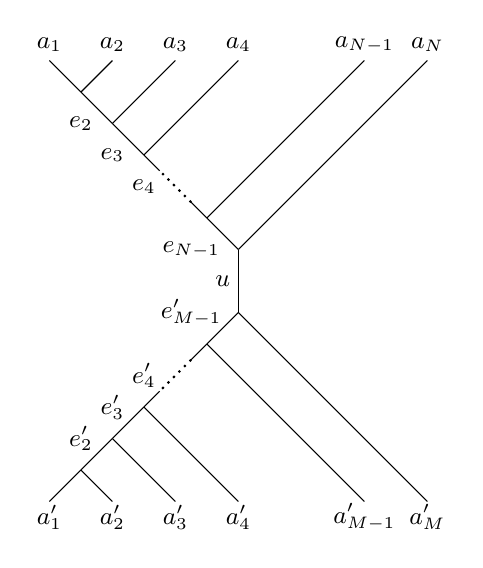
\begin{tikzpicture}[scale=0.8,baseline=(current bounding box.center)]
			\draw (0,0) -- (0,0.5);
			\draw (0,0.5) -- (-0.5,1);
			\draw (-0.5,1) -- (-0.75,1.25);
			\draw[dotted,thick] (-0.75,1.25) -- (-1.25,1.75);
			\draw (-1.25,1.75) -- (-1.5,2);
			\draw (-1.5,2) -- (-2,2.5);
			\draw (-2,2.5) -- (-2.5,3);
			\draw (-2.5,3) -- (-3,3.5);
			\draw (0,0.5) -- (3,3.5);
			\draw (-0.5,1) -- (2,3.5);
			\draw (-1.5,2) -- (0,3.5);
			\draw (-2,2.5) -- (-1,3.5);
			\draw (-2.5,3) -- (-2,3.5);
			\node at (-0.25,0) {\small $u$};
			\node at (-0.75,0.5) {\small $e_{N-1}$};
			\node at (-2,2) {\small $e_3$};
			\node at (-2.5,2.5) {\small $e_2$};
			\node at (-1.5,1.5) {\small $e_4$};
			\node at (-3,3.75) {\small $a_1$};
			\node at (-2,3.75) {\small $a_2$};
			\node at (-1,3.75) {\small $a_3$};
			\node at (0,3.75) {\small $a_4$};
			\node at (2,3.75) {\small $a_{N-1}$};
			\node at (3,3.75) {\small $a_N$};
			\begin{scope}[yscale=-1]
			\draw (0,0) -- (0,0.5);
			\draw (0,0.5) -- (-0.5,1);
			\draw (-0.5,1) -- (-0.75,1.25);
			\draw[dotted,thick] (-0.75,1.25) -- (-1.25,1.75);
			\draw (-1.25,1.75) -- (-1.5,2);
			\draw (-1.5,2) -- (-2,2.5);
			\draw (-2,2.5) -- (-2.5,3);
			\draw (-2.5,3) -- (-3,3.5);
			\draw (0,0.5) -- (3,3.5);
			\draw (-0.5,1) -- (2,3.5);
			\draw (-1.5,2) -- (0,3.5);
			\draw (-2,2.5) -- (-1,3.5);
			\draw (-2.5,3) -- (-2,3.5);
			\node at (-0.75,0.5) {\small $e_{M-1}'$};
			\node at (-2,2) {\small $e_3'$};
			\node at (-2.5,2.5) {\small $e_2'$};
			\node at (-1.5,1.5) {\small $e_4'$};
			\node at (-3,3.75) {\small $a_1'$};
			\node at (-2,3.75) {\small $a_2'$};
			\node at (-1,3.75) {\small $a_3'$};
			\node at (0,3.75) {\small $a_4'$};
			\node at (2,3.75) {\small $a_{M-1}'$};
			\node at (3,3.75) {\small $a_M'$};
			\end{scope}
		\end{tikzpicture}.
	\end{equation}
We usually use the normalisation convention
	\begin{equation}
	\label{eq:vertexnorm}
		\left(\frac{d_c}{d_a d_b}\right)^\frac{1}{4}
		\begin{tikzpicture}[scale=0.5,baseline=(current bounding box.center),yscale=-1]
		\node at (-0.55,-0.65) {$\psi$};
		\draw (0,0) -- (0,-1);
		\draw (0,-1) -- (-1,-2);
		\draw (0,-1) -- (1,-2);
		\node at (0,0.4) {$c$};
		\node at (-1.1,-2.4) {$a$};
		\node at (1.1,-2.4) {$b$};
		\end{tikzpicture}\in V^{ab}_c,\hspace{30pt}
		\left(\frac{d_c}{d_a d_b}\right)^\frac{1}{4}
		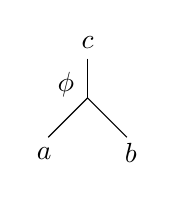
\begin{tikzpicture}[scale=0.5,baseline=(current bounding box.center)]
		\node at (-0.55,-0.65) {$\phi$};
		\draw (0,0) -- (0,-1);
		\draw (0,-1) -- (-1,-2);
		\draw (0,-1) -- (1,-2);
		\node at (0,0.4) {$c$};
		\node at (-1.1,-2.4) {$a$};
		\node at (1.1,-2.4) {$b$};
		\end{tikzpicture}\in V_{ab}^c
	\end{equation}
for trivalent vertices throughout this thesis. Using this convention, the identity operation on two particles $a$ and $b$ can be decomposed in the following way:
	\begin{equation}
	\label{eq:identity}
		\begin{tikzpicture}[scale=0.9,baseline=(current bounding box.center)]
			\node at (0,0) {\small $a$};
			\node at (1,0) {\small $b$};
			\node at (0,2.5) {\small $a$};
			\node at (1,2.5) {\small $b$};
			\draw (0,0.25) -- (0,2.25);
			\draw (1,0.25) -- (1,2.25);
		\end{tikzpicture}=\sum_c\sum_\alpha \sqrt{\frac{d_c}{d_a d_b}}
		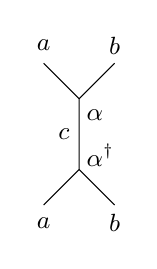
\begin{tikzpicture}[scale=0.9,baseline=(current bounding box.center)]
			\node at (0,0) {\small $a$};
			\node at (1,0) {\small $b$};
			\node at (0,2.5) {\small $a$};
			\node at (1,2.5) {\small $b$};
			\draw (0,0.25) -- (0.5,0.75) to node[left] {\small $c$} (0.5,1.75) -- (0,2.25);
			\draw (1,0.25) -- (0.5,0.75);
			\draw (1,2.25) -- (0.5,1.75);
			\node at (0.8,0.95) {\small $\alpha^\dagger$};
			\node at (0.8,1.6) {\small $\alpha\phantom{^\dagger}$};
		\end{tikzpicture}.
	\end{equation}
The sum over $\alpha$ can be neglected if the fusion rules are multiplicity-free. This relation is also called the \emph{completeness relation}\index{completeness relation}.

Furthermore, the inner product of two vectors is diagrammatically formed by stacking vertices on top of each other such that the fusion/splitting lines connect. The simplest case is the so-called \emph{bigon relation}\index{bigon relation}:
	\begin{equation}
	\label{eq:bigon2}
		\begin{tikzpicture}[baseline=(current bounding box.center)]
			\draw (0,0) -- (0,0.5);
			\draw (0,0.5) to[bend left=60] node[left] {$a$} (0,1.5);
			\draw (0,0.5) to[bend right=60] node[right] {$b$} (0,1.5);
			\draw (0,1.5) -- (0,2);
			\node at (0,-0.25) {$c$};
			\node at (0,2.25) {$c'$};
		\end{tikzpicture}=\delta_{c,c'}\sqrt{\frac{d_a d_b}{d_c}}\ 
		\begin{tikzpicture}[baseline=(current bounding box.center)]
			\draw (0,0) to node[right] {$c$} (0,2);
		\end{tikzpicture}.
	\end{equation}
This generalizes to more complicated diagrams. From this formula, we can directly see that tadpole diagrams (``lollipops''), i.e., diagrams of the form
	\begin{equation}
		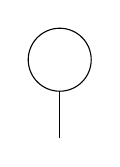
\begin{tikzpicture}
			\draw (0,0) -- (0,0.6);
			\draw (0,1) circle (0.4cm);
		\end{tikzpicture}
	\end{equation}
are forbidden, since these kind of diagrams correspond to the case $c'=\mathbf{1}$ and therefore
	\begin{equation}
		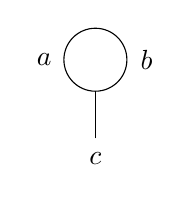
\begin{tikzpicture}[baseline=(current bounding box.center)]
			\draw (0,0) -- (0,0.6);
			\draw (0,1) circle (0.4cm);
			\node at (0,-0.25) {$c$};
			\node at (-0.65,1) {$a$};
			\node at (0.65,1) {$b$};
		\end{tikzpicture}\equiv
		\begin{tikzpicture}[baseline=(current bounding box.center)]
			\draw (0,0) -- (0,0.5);
			\draw (0,0.5) to[bend left=60] node[left] {$a$} (0,1.5);
			\draw (0,0.5) to[bend right=60] node[right] {$b$} (0,1.5);
			\draw[dashed] (0,1.5) -- (0,2);
			\node at (0,-0.25) {$c$};
			\node at (0,2.25) {$\mathbf{1}$};
		\end{tikzpicture}=\delta_{c,\mathbf{1}}\sqrt{\frac{d_a d_b}{d_c}}\ 
		\begin{tikzpicture}[baseline=(current bounding box.center)]
			\draw (0,0) to node[right] {$c$} (0,2);
		\end{tikzpicture},
	\end{equation}
where the right hand side is only non-zero for $c=\mathbf{1}$.

In the following, we will focus on describing properties of splitting spaces since these are the ones that will mainly appear in this thesis. Note that all statements can analogously be made for fusion spaces.

Categorically, to be able to work with the tree diagrams as they are introduced above, we need to choose bases for the involved morphism spaces. Furthermore, as described in \cref{ch:cats}, transforming between different bases is done by applying the correct $F$-matrices\index{F-symbol@$F$-symbol}. Recall that these matrices are defined via the equation
	\begin{equation}
		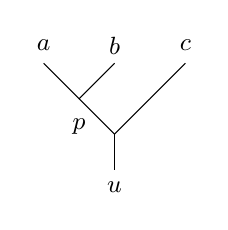
\begin{tikzpicture}[baseline=(current bounding box.center),yscale=0.9,xscale=0.9]
			\draw (0,0.5) -- (0,1);
			\draw (0,1) -- (-0.5,1.5);
			\draw (-0.5,1.5) -- (-1,2);
			\draw (-0.5,1.5) -- (0,2);
			\draw (0,1) -- (0.5,1.5);
			\draw (0.5,1.5) -- (1,2);
			\node at (0,0.25) {\small $u$};
			\node at (-1,2.25) {\small $a$};
			\node at (0,2.25) {\small $b$};
			\node at (1,2.25) {\small $c$};
			\node at (-0.5,1.1) {\small $p$};
		\end{tikzpicture}=\sum_q \left(F_u^{abc}\right)_{qp}
		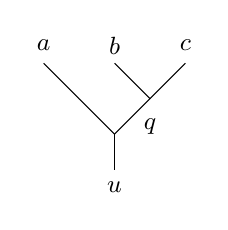
\begin{tikzpicture}[baseline=(current bounding box.center),yscale=0.9,xscale=0.9]
			\draw (0,0.5) -- (0,1);
			\draw (0,1) -- (-0.5,1.5);
			\draw (-0.5,1.5) -- (-1,2);
			\draw (0.5,1.5) -- (0,2);
			\draw (0,1) -- (0.5,1.5);
			\draw (0.5,1.5) -- (1,2);
			\node at (0,0.25) {\small $u$};
			\node at (-1,2.25) {\small $a$};
			\node at (0,2.25) {\small $b$};
			\node at (1,2.25) {\small $c$};
			\node at (0.5,1.1) {\small $q$};
		\end{tikzpicture}.
	\end{equation}
Here, the diagram on the left-hand side is in the standard form we have chosen for tree diagrams. In the context of anyons, the above relation can also be motivated from a different point of view than the purely mathematical one: The two different bases both correspond to the splitting of a particle $u$ into the three particles $a,b,c$. Since by fusion we do not mean a physical process, but rather a grouping of particles into one system whose statistical behaviour we are interested in, these two choices are physically the same and are therefore connected via a unitary isomorphism, which is given by the $F$-matrices. 

Recall that the $F$-matrices have to fulfil a consistency condition, the so-called pentagon equation \cref{eq:pentagon}. Furthermore, in a unitary fusion category there are some additional relations between diagrams in terms of $F$-symbols. First, in a unitary fusion category the inverse of an $F$-symbol is given by the hermitian conjugate:
	\begin{equation}
		\left(F_u^{abc}\right)_{qp}^{-1}=\left(F_u^{abc}\right)_{qp}^\dagger=\overline{\Big(F_u^{abc}\Big)}_{pq}.
	\end{equation}
In terms of string diagrams, this means that
	\begin{equation}
		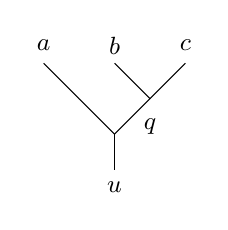
\begin{tikzpicture}[baseline=(current bounding box.center),yscale=0.9,xscale=0.9]
			\draw (0,0.5) -- (0,1);
			\draw (0,1) -- (-0.5,1.5);
			\draw (-0.5,1.5) -- (-1,2);
			\draw (0.5,1.5) -- (0,2);
			\draw (0,1) -- (0.5,1.5);
			\draw (0.5,1.5) -- (1,2);
			\node at (0,0.25) {\small $u$};
			\node at (-1,2.25) {\small $a$};
			\node at (0,2.25) {\small $b$};
			\node at (1,2.25) {\small $c$};
			\node at (0.5,1.1) {\small $q$};
		\end{tikzpicture}=\sum_p \left(F_u^{abc}\right)_{pq}^\dagger
		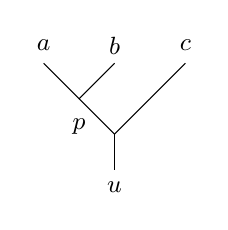
\begin{tikzpicture}[baseline=(current bounding box.center),yscale=0.9,xscale=0.9]
			\draw (0,0.5) -- (0,1);
			\draw (0,1) -- (-0.5,1.5);
			\draw (-0.5,1.5) -- (-1,2);
			\draw (-0.5,1.5) -- (0,2);
			\draw (0,1) -- (0.5,1.5);
			\draw (0.5,1.5) -- (1,2);
			\node at (0,0.25) {\small $u$};
			\node at (-1,2.25) {\small $a$};
			\node at (0,2.25) {\small $b$};
			\node at (1,2.25) {\small $c$};
			\node at (-0.5,1.1) {\small $p$};
		\end{tikzpicture}.
	\end{equation}
Another consequence of unitarity is that the category is automatically spherical\index{spherical category} (see \cite[Proposition 8.23]{Etingof2005}), which yields a so-called \emph{mirror symmetry}\index{mirror symmetry} (see \cite{Hong2009}). This means that we can find relations between horizontally mirrored tree diagrams in terms of the previously defined $F$-symbols:
	\begin{align}
		\begin{tikzpicture}[baseline=(current bounding box.center),yscale=-0.9,xscale=0.9]
			\draw (0,0.5) -- (0,1);
			\draw (0,1) -- (-0.5,1.5);
			\draw (-0.5,1.5) -- (-1,2);
			\draw (-0.5,1.5) -- (0,2);
			\draw (0,1) -- (0.5,1.5);
			\draw (0.5,1.5) -- (1,2);
			\node at (0,0.25) {\small $u$};
			\node at (-1,2.25) {\small $a$};
			\node at (0,2.25) {\small $b$};
			\node at (1,2.25) {\small $c$};
			\node at (-0.5,1.1) {\small $p$};
		\end{tikzpicture}&=\sum_q \overline{\left(F_u^{abc}\right)}_{qp}
		\begin{tikzpicture}[baseline=(current bounding box.center),yscale=-0.9,xscale=0.9]
			\draw (0,0.5) -- (0,1);
			\draw (0,1) -- (-0.5,1.5);
			\draw (-0.5,1.5) -- (-1,2);
			\draw (0.5,1.5) -- (0,2);
			\draw (0,1) -- (0.5,1.5);
			\draw (0.5,1.5) -- (1,2);
			\node at (0,0.25) {\small $u$};
			\node at (-1,2.25) {\small $a$};
			\node at (0,2.25) {\small $b$};
			\node at (1,2.25) {\small $c$};
			\node at (0.5,1.1) {\small $q$};
		\end{tikzpicture}\\
		\begin{tikzpicture}[baseline=(current bounding box.center),yscale=-0.9,xscale=0.9]
			\draw (0,0.5) -- (0,1);
			\draw (0,1) -- (-0.5,1.5);
			\draw (-0.5,1.5) -- (-1,2);
			\draw (0.5,1.5) -- (0,2);
			\draw (0,1) -- (0.5,1.5);
			\draw (0.5,1.5) -- (1,2);
			\node at (0,0.25) {\small $u$};
			\node at (-1,2.25) {\small $a$};
			\node at (0,2.25) {\small $b$};
			\node at (1,2.25) {\small $c$};
			\node at (0.5,1.1) {\small $q$};
		\end{tikzpicture}&=\sum_p \left(F_u^{abc}\right)_{pq}^\mathrm{T}
		\begin{tikzpicture}[baseline=(current bounding box.center),yscale=-0.9,xscale=0.9]
			\draw (0,0.5) -- (0,1);
			\draw (0,1) -- (-0.5,1.5);
			\draw (-0.5,1.5) -- (-1,2);
			\draw (-0.5,1.5) -- (0,2);
			\draw (0,1) -- (0.5,1.5);
			\draw (0.5,1.5) -- (1,2);
			\node at (0,0.25) {\small $u$};
			\node at (-1,2.25) {\small $a$};
			\node at (0,2.25) {\small $b$};
			\node at (1,2.25) {\small $c$};
			\node at (-0.5,1.1) {\small $p$};
		\end{tikzpicture}.
	\end{align}
Furthermore, in any spherical category $\C$ it holds for the quantum dimension of any object $a\in\Obj(\C)$ that $d_{a^*}=d_a$.

\begin{rem}
	\label{rem:Felements}
	Because the $F$-symbol is a transformation between two different bases, the graphical calculus of fusion categories allows us to calculate matrix elements $\left(F_u^{abc}\right)_{qp}$ via the scalar product of elements of the respective orthonormal bases. For this purpose, the orthonormal bases we use are 
		\begin{equation}
			\left\{\frac{1}{\left(d_ad_bd_cd_u\right)^{\frac{1}{4}}}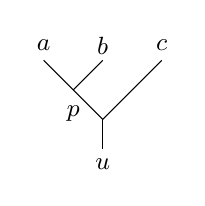
\begin{tikzpicture}[baseline=(current bounding box.center),yscale=0.75,xscale=0.75]
				\draw (0,0.5) -- (0,1);
				\draw (0,1) -- (-0.5,1.5);
				\draw (-0.5,1.5) -- (-1,2);
				\draw (-0.5,1.5) -- (0,2);
				\draw (0,1) -- (0.5,1.5);
				\draw (0.5,1.5) -- (1,2);
				\node at (0,0.25) {\small $u$};
				\node at (-1,2.25) {\small $a$};
				\node at (0,2.25) {\small $b$};
				\node at (1,2.25) {\small $c$};
				\node at (-0.5,1.1) {\small $p$};
			\end{tikzpicture}\right\}\hspace{10pt}\mathrm{and}\hspace{10pt}
			\left\{\frac{1}{\left(d_ad_bd_cd_u\right)^{\frac{1}{4}}}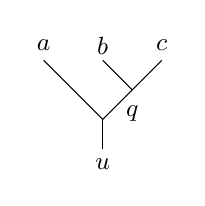
\begin{tikzpicture}[baseline=(current bounding box.center),yscale=0.75,xscale=0.75]
				\draw (0,0.5) -- (0,1);
				\draw (0,1) -- (-0.5,1.5);
				\draw (-0.5,1.5) -- (-1,2);
				\draw (0.5,1.5) -- (0,2);
				\draw (0,1) -- (0.5,1.5);
				\draw (0.5,1.5) -- (1,2);
				\node at (0,0.25) {\small $u$};
				\node at (-1,2.25) {\small $a$};
				\node at (0,2.25) {\small $b$};
				\node at (1,2.25) {\small $c$};
				\node at (0.5,1.1) {\small $q$};
			\end{tikzpicture}\right\}.
		\end{equation}
	The normalisation factor $\frac{1}{\left(d_ad_bd_cd_u\right)^{\frac{1}{4}}}$ comes from the normalisation of vertices we chose in \cref{eq:vertexnorm} together with an additional factor of $\frac{1}{\sqrt{d_u}}$ in order to make the diagram normalised with respect to the trace defined in \cref{def:trace}. The calculation of the matrix element then works via the scalar product of two basis elements:	
		\begin{align}
			\left(F_u^{abc}\right)_{qp}&=\frac{1}{\sqrt{d_a d_b d_c d_u}}
			\Bigg\langle
			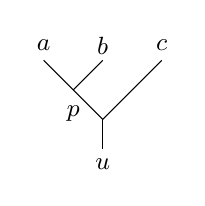
\begin{tikzpicture}[baseline=(current bounding box.center),yscale=0.75,xscale=0.75]
				\draw (0,0.5) -- (0,1);
				\draw (0,1) -- (-0.5,1.5);
				\draw (-0.5,1.5) -- (-1,2);
				\draw (-0.5,1.5) -- (0,2);
				\draw (0,1) -- (0.5,1.5);
				\draw (0.5,1.5) -- (1,2);
				\node at (0,0.25) {\small $u$};
				\node at (-1,2.25) {\small $a$};
				\node at (0,2.25) {\small $b$};
				\node at (1,2.25) {\small $c$};
				\node at (-0.5,1.1) {\small $p$};
			\end{tikzpicture}
			\Bigg|
			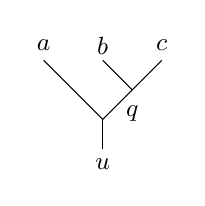
\begin{tikzpicture}[baseline=(current bounding box.center),yscale=0.75,xscale=0.75]
				\draw (0,0.5) -- (0,1);
				\draw (0,1) -- (-0.5,1.5);
				\draw (-0.5,1.5) -- (-1,2);
				\draw (0.5,1.5) -- (0,2);
				\draw (0,1) -- (0.5,1.5);
				\draw (0.5,1.5) -- (1,2);
				\node at (0,0.25) {\small $u$};
				\node at (-1,2.25) {\small $a$};
				\node at (0,2.25) {\small $b$};
				\node at (1,2.25) {\small $c$};
				\node at (0.5,1.1) {\small $q$};
			\end{tikzpicture}
			\Bigg\rangle\\
			&=\frac{1}{\sqrt{d_a d_b d_c d_u}}
			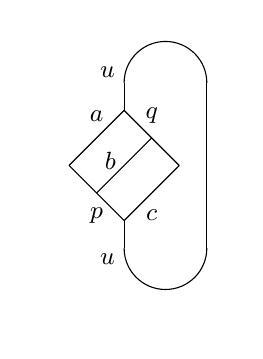
\begin{tikzpicture}[baseline=(j.base),scale=0.7]
				\clip(-1.75,-1) rectangle (2,4.5);
				\draw (0,0.5) -- (0,1);
				\draw (0,1) -- (-0.5,1.5);
				\coordinate (j) at (-1,2);
				\draw (-0.5,1.5) -- (j);
				\draw (-0.5,1.5) -- node[above] {\small $b$} (0,2);
				\draw (0,1) -- (0.5,1.5);
				\draw (0.5,1.5) -- (1,2);
				\node at (-0.5,1.1) {\small $p$};
				\node at (0.5,1.1) {\small $c$};
				\draw (0,0.5) arc (-180:0:0.75cm);
				\rotatebox[]{180}{
					\begin{scope}[yshift=-4cm]
					\draw (0,0.5) -- (0,1);
					\draw (0,1) -- (-0.5,1.5);
					\draw (-0.5,1.5) -- (-1,2);
					\draw (-0.5,1.5) -- (0,2);
					\draw (0,1) -- (0.5,1.5);
					\draw (0.5,1.5) -- (1,2);
					\node at (-0.5,1.1) {\rotatebox[]{180}{\small $q$}};
					\node at (0.5,1.1) {\rotatebox[]{180}{\small $a$}};
					\draw (0,0.5) arc (0:-180:0.75cm);
					\end{scope}
				}
				\draw (1.5,0.5) -- (1.5,3.5);
				\node at (-0.3,0.3) {\small $u$};
				\node at (-0.3,3.7) {\small $u$};
			\end{tikzpicture}\\
			&=\frac{1}{\sqrt{d_a d_b d_c d_u}}\sum_{p'}\left(F_u^{abc}\right)_{p'p}
			\begin{tikzpicture}[baseline=(j.base),scale=0.7]
				\clip(-1.75,-1) rectangle (2,4.5);
				\draw (0,0.5) -- (0,1);
				\draw (0,1) -- (-0.5,1.5);
				\draw (-0.5,1.5) -- node[left] {\small $a$} (-1,2);
				\draw (0.5,1.5) -- node[left] {\small $b$} (0,2);
				\draw (0,1) -- (0.5,1.5);
				\draw (0.5,1.5) -- node[right] {\small $c$} (1,2);
				%\node at (-0.5,1.1) {\small $m$};
				\node at (0.5,1.1) {\small $p'$};
				\draw (0,0.5) arc (-180:0:0.75cm);
				\rotatebox[]{180}{
					\begin{scope}[yshift=-4cm]
					\draw (0,0.5) -- (0,1);
					\draw (0,1) -- (-0.5,1.5);
					\draw (-0.5,1.5) -- (-1,2);
					\draw (-0.5,1.5) -- (0,2);
					\draw (0,1) -- (0.5,1.5);
					\draw (0.5,1.5) -- (1,2);
					\node at (-0.5,1.1) {\rotatebox[]{180}{\small $q$}};
					%\node at (0.5,1.1) {\rotatebox[]{180}{\small $j$}};
					\draw (0,0.5) arc (0:-180:0.75cm);
					\end{scope}
				}
				\draw (1.5,0.5) -- (1.5,3.5);
				\node at (-0.3,0.3) {\small $u$};
				\node at (-0.3,3.7) {\small $u$};
			\end{tikzpicture}\\
			&=\frac{1}{\sqrt{d_a d_b d_c d_u}}\left(F_u^{abc}\right)_{qp}\sqrt{\frac{d_b d_c}{d_q}} \sqrt{\frac{d_a d_q}{d_u}}\ d_u\\
			&=\left(F_u^{abc}\right)_{qp},
		\end{align}
	where we have applied the bigon relation \cref{eq:bigon2} twice and also used that the loop value is the quantum dimension, which will be explained in \cref{eq:qdimgraph}.
\end{rem}

In the context of physical models, apart from ensuring that the $F$-moves themselves are consistent, it is also crucial that adding and removing vacuum lines is consistent with the $F$-moves. From a physical perspective, splitting from or fusing with the vacuum is trivial. This is the reason why we can always add an remove vacuum lines in tree diagrams. To guarantee the consistency of this procedure with the model (especially with the $F$-moves), we require that the vector spaces $V_{a}^{a\mathbf{1}}$ and $V_a^{\mathbf{1}a}$ are one-dimensional and, furthermore, that they are canonically isomorphic to $\mathbb{C}$. In other words, these vector spaces have fixed unit vectors $\alpha_a\in V_a^{a\mathbf{1}}$ and $\beta_a\in V_a^{\mathbf{1}a}$. The canonical isomorphisms are simply given by
	\begin{alignat}{3}
		\alpha_a:\mathbb{C}&\to V_a^{a\mathbf{1}},\hspace{20pt}\beta_a:\ &\mathbb{C}\,&\to V_a^{\mathbf{1}a}\\
		z&\mapsto z\alpha_a, &z\,&\mapsto z\beta_a
	\end{alignat}
These isomorphisms have to fulfil the so-called \emph{triangle equation}\index{triangle equation} depicted in \cref{fig:triangle_eq}\,\textbf{(a)} to ensure consistency with the $F$-moves. There are two corollaries of the triangle equation, depicted in \cref{fig:triangle_eq}\,\textbf{(b)} and \textbf{(c)}, which automatically follow from the first triangle equation and the pentagon equation.

	\begin{figure}[t]
		\centering
		\begin{tikzpicture}[xscale=0.4,yscale=0.4]
			\node at (-7,1.5) {\textbf{(a)}};
			\node at (0,-1.4) {\small $u$};
			\node at (-1,1.4) {\small $a$};
			\node at (1,1.4) {\small $b$};
			\draw (0,-1) -- (0,0);
			\draw (0,0) -- (-1,1);
			\draw (0,0) -- (1,1);
			\node at (-5,-8.4) {\small $u$};
			\node at (-7,-4.6) {\small $a$};
			\node at (-5,-4.6) {\small $\mathbf{1}$};
			\node at (-3,-4.6) {\small $b$};
			\draw (-5,-8) -- (-5,-7);
			\draw (-5,-7) -- (-6,-6);
			\draw (-5,-7) -- (-4,-6);
			\draw (-6,-6) -- (-7,-5);
			\draw[dashed] (-6,-6) -- (-5,-5);
			\draw (-4,-6) -- (-3,-5);
			\node at (5,-8.4) {\small $u$};
			\node at (7,-4.6) {\small $b$};
			\node at (5,-4.6) {\small $\mathbf{1}$};
			\node at (3,-4.6) {\small $a$};
			\draw (5,-8) -- (5,-7);
			\draw (5,-7) -- (6,-6);
			\draw (5,-7) -- (4,-6);
			\draw (6,-6) -- (7,-5);
			\draw[dashed] (6,-6) -- (5,-5);
			\draw (4,-6) -- (3,-5);
			\draw[->,>=stealth] (-2,-7) -- node[above] {$F_u^{a\mathbf{1}b}$} (2,-7);
			\draw[->,>=stealth] (-2,-1) -- node[left,near start] {$\alpha_a\ $} (-4,-3);
			\draw[->,>=stealth] (2,-1) -- node[right,near start] {$\ \ \beta_b$} (4,-3);
		\end{tikzpicture}\\[20pt]
		\begin{tikzpicture}[xscale=0.4,yscale=0.4]
			\node at (-7,1.5) {\textbf{(b)}};
			\node at (0,-1.4) {\small $u$};
			\node at (-1,1.4) {\small $a$};
			\node at (1,1.4) {\small $b$};
			\draw (0,-1) -- (0,0);
			\draw (0,0) -- (-1,1);
			\draw (0,0) -- (1,1);
			\node at (-5,-8.4) {\small $u$};
			\node at (-7,-4.6) {\small $\mathbf{1}$};
			\node at (-5,-4.6) {\small $a$};
			\node at (-3,-4.6) {\small $b$};
			\draw (-5,-8) -- (-5,-7);
			\draw (-5,-7) -- (-6,-6);
			\draw (-5,-7) -- (-4,-6);
			\draw[dashed] (-6,-6) -- (-7,-5);
			\draw (-6,-6) -- (-5,-5);
			\draw (-4,-6) -- (-3,-5);
			\node at (5,-8.4) {\small $u$};
			\node at (7,-4.6) {\small $b$};
			\node at (5,-4.6) {\small $a$};
			\node at (3,-4.6) {\small $\mathbf{1}$};
			\draw (5,-8) -- (5,-7);
			\draw (5,-7) -- (6,-6);
			\draw[dashed] (5,-7) -- (4,-6);
			\draw (6,-6) -- (7,-5);
			\draw (6,-6) -- (5,-5);
			\draw[dashed] (4,-6) -- (3,-5);
			\draw[->,>=stealth] (-2,-7) -- node[above] {$F_u^{\mathbf{1}ab}$} (2,-7);
			\draw[->,>=stealth] (-2,-1) -- node[left,near start] {$\beta_a\ $} (-4,-3);
			\draw[->,>=stealth] (2,-1) -- node[right,near start] {$\ \ \beta_u$} (4,-3);
		\end{tikzpicture}\hspace{20pt}
		\begin{tikzpicture}[xscale=0.4,yscale=0.4]
			\node at (-7,1.5) {\textbf{(c)}};
			\node at (0,-1.4) {\small $u$};
			\node at (-1,1.4) {\small $a$};
			\node at (1,1.4) {\small $b$};
			\draw (0,-1) -- (0,0);
			\draw (0,0) -- (-1,1);
			\draw (0,0) -- (1,1);
			\node at (-5,-8.4) {\small $u$};
			\node at (-7,-4.6) {\small $a$};
			\node at (-5,-4.6) {\small $b$};
			\node at (-3,-4.6) {\small $\mathbf{1}$};
			\draw (-5,-8) -- (-5,-7);
			\draw (-5,-7) -- (-6,-6);
			\draw[dashed] (-5,-7) -- (-4,-6);
			\draw (-6,-6) -- (-7,-5);
			\draw (-6,-6) -- (-5,-5);
			\draw[dashed] (-4,-6) -- (-3,-5);
			\node at (5,-8.4) {\small $u$};
			\node at (7,-4.6) {\small $\mathbf{1}$};
			\node at (5,-4.6) {\small $b$};
			\node at (3,-4.6) {\small $a$};
			\draw (5,-8) -- (5,-7);
			\draw (5,-7) -- (6,-6);
			\draw (5,-7) -- (4,-6);
			\draw[dashed] (6,-6) -- (7,-5);
			\draw (6,-6) -- (5,-5);
			\draw (4,-6) -- (3,-5);
			\draw[->,>=stealth] (-2,-7) -- node[above] { $F_u^{ab\mathbf{1}}$} (2,-7);
			\draw[->,>=stealth] (-2,-1) -- node[left,near start] {$\alpha_u\ $} (-4,-3);
			\draw[->,>=stealth] (2,-1) -- node[right,near start] {$\ \ \alpha_b$} (4,-3);
		\end{tikzpicture}		
		\caption{\small \textbf{Diagrammatic depiction of the triangle equation.} \textbf{(a)} The triangle equation ensures that fusion with/splitting from the vacuum lines is compatible with the $F$-move. \textbf{(b)} and \textbf{(c)} are corollaries of the triangle equation that are automatically implied by equation \textbf{(a)} and the pentagon equation.}
		\label{fig:triangle_eq}
	\end{figure}


\subsection*{Bending and tracing.}

We often want to introduce and remove bends in a line. Horizontal bending of lines (such that the line always goes upwards) is trivial:
	\begin{equation}
		\begin{tikzpicture}[scale=0.9,baseline=(current bounding box.center)]
			\draw (0,0) to node[right] {$a$} (0,2);
		\end{tikzpicture}\ =\ 
		\begin{tikzpicture}[scale=0.8,baseline=(current bounding box.center)]
			\begin{knot}[consider self intersections=true,ignore endpoint intersections=false]
			\strand (0,0) -- (0,0.25) to[out=90,in=270] (0.25,1) to[out=90,in=270] (0,1.75) -- (0,2);
			\end{knot}
			\node at (0.5,1) {$a$};
		\end{tikzpicture}.
	\end{equation}
In contrast, one has to be very careful when bending lines vertically, for example transformations such as the following:
	\begin{equation}
		\begin{tikzpicture}[scale=0.75,baseline=(current bounding box.center)]
			\draw (0,-0.25) to node[left] {\small $a$} (0,2.25);
		\end{tikzpicture}\ \to\ 
		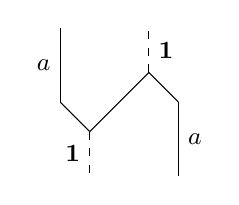
\begin{tikzpicture}[scale=0.75,baseline=(current bounding box.center)]
			\draw (0,0) to node[left] {\small $a$} (0,1.25);
			\draw (0,0) -- (0.5,-0.5);
			\draw (0.5,-0.5) -- (1.5,0.5);
			\draw (1.5,0.5) -- (2,0);
			\draw (2,0) to node[right] {\small $a$} (2,-1.25);
			\draw[dashed] (0.5,-0.5) to node[left] {\small $\mathbf{1}$} (0.5,-1.25);
			\draw[dashed] (1.5,0.5) to node[right] {\small $\mathbf{1}$} (1.5,1.25);
		\end{tikzpicture}.
	\end{equation}
Recall that we are free to bend lines horizontally (as explained above) and, furthermore, are allowed to add and remove vacuum lines. Therefore we can modify the above diagram such that we can apply $F$-moves in order to evaluate the effect of bending lines vertically:
	\begin{equation}
	\label{eq:FrobSchur}
		\begin{tikzpicture}[baseline=(current bounding box.center)]
			\draw (0,0) -- (0,0.5);
			\draw (0,0.5) -- (1,1.5);
			\draw[dashed] (0,0.5) to node[left, near start] {\small $\mathbf{1}\ $} (-0.5,1);
			\draw (1,1.5) -- (0.5,2);
			\draw (0.5,2) -- (-0.5,1);
			\draw[dashed] (0.5,2) to node[right, near end] {\small $\ \mathbf{1}$} (0,2.5);
			\draw (-0.5,1) -- (-1,1.5);
			\draw (-1,1.5) -- (0,2.5);
			\draw (0,2.5) -- (0,3);
			\node at (0,-0.25) {\small $a$};
			\node at (0,3.25) {\small $a$};
			\node at (1.25,1.5) {\small $a$};
			\node at (-1.25,1.5) {\small $a$};
			\node at (0.25,1.5) {\small $a^*$};
		\end{tikzpicture}=\sum_x\left(F_a^{aa^*a}\right)_{x\mathbf{1}}
		\begin{tikzpicture}[baseline=(current bounding box.center)]
			\draw (0,0) -- (0,0.5);
			\draw (0,0.5) -- (1,1.5);
			\draw (0,0.5) -- (-0.5,1);
			\draw (1,1.5) -- (0.5,2);
			\draw (0.5,2) -- (0,1.5) -- (0.5,1);
			\draw[dashed] (0.5,2) to node[right, near end] {\small $\ \mathbf{1}$} (0,2.5);
			\draw (-0.5,1) -- (-1,1.5);
			\draw (-1,1.5) -- (0,2.5);
			\draw (0,2.5) -- (0,3);
			\node at (0,-0.25) {\small $a$};
			\node at (0,3.25) {\small $a$};
			\node at (1.25,1.5) {\small $a$};
			\node at (-1.25,1.5) {\small $a$};
			\node at (-0.25,1.5) {\small $a^*$};
			\node at (0.45,0.65) {\small $x$};
		\end{tikzpicture}=d_a\left(F_a^{aa^*a}\right)_{\mathbf{1}\mathbf{1}}\ 
		\begin{tikzpicture}[baseline=(current bounding box.center)]
			\draw (0,0) to node[right] {$a$} (0,3);
		\end{tikzpicture},
	\end{equation}
where we have used \cref{eq:bigon2} twice in the last step. Here, the quantity
	\begin{equation}
	\label{eq:FrobSchur2}
		\left(F_a^{aa^*a}\right)_{\mathbf{1}\mathbf{1}}=\frac{\kappa_a}{d_a}
	\end{equation}
has, in general, a non-trivial phase $\kappa_a=\kappa_{a^*}^*$. It is always possible to find a gauge choice such that $\kappa_a=1$ for all self-dual particle types $a$ (i.e., for particles with $a=a^*$), but for those particle types that are not self-dual, $\kappa_a=\pm 1$ is the \emph{Frobenius-Schur indicator}\index{Frobenius-Schur indicator}, which is a gauge-invariant quantity. This is the reason why bending lines vertically is more intricate than bending them horizontally. 

One possible way to account for this problem is by introducing \emph{flags} (following the notation in \cite{kitaev_anyons_2006} and \cite{Bond2007}): When removing a vacuum line from the top of a fusion vertex or from the bottom of a splitting vertex, we indicate this by drawing a right-directed flag:
	\begin{align}
	\label{eq:evaluationcat}
		\begin{tikzpicture}[baseline=(current bounding box.center)]
			\draw (0,0) -- (0.5,0.5) -- (1,0);
			\draw[dashed] (0.5,0.5) -- (0.5,1);
			\node at (0,-0.25) {$a$};
			\node at (1,-0.25) {$a^*$};
			\node at (0.5,1.25) {$\mathbf{1}$};
		\end{tikzpicture}\ &=\ 
		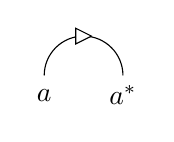
\begin{tikzpicture}[baseline=(current bounding box.center)]
			\draw (0,0) arc (180:0:0.5);
			\draw[fill=white] (0.6,0.5) -- (0.4,0.6) -- (0.4,0.4) -- cycle;
			\node at (0,-0.25) {$a$};
			\node at (1,-0.25) {$a^*$};
		\end{tikzpicture}\ =\kappa_a\ 
		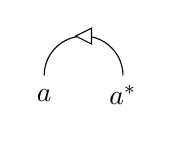
\begin{tikzpicture}[baseline=(current bounding box.center)]
			\draw (0,0) arc (180:0:0.5);
			\draw[fill=white] (0.4,0.5) -- (0.6,0.4) -- (0.6,0.6) -- cycle;
			\node at (0,-0.25) {$a$};
			\node at (1,-0.25) {$a^*$};
		\end{tikzpicture}\\
		\label{eq:coevaluationcat}
		\begin{tikzpicture}[baseline=(current bounding box.center),yscale=-1]
			\draw (0,0) -- (0.5,0.5) -- (1,0);
			\draw[dashed] (0.5,0.5) -- (0.5,1);
			\node at (0,-0.25) {$a$};
			\node at (1,-0.25) {$a^*$};
			\node at (0.5,1.25) {$\mathbf{1}$};
		\end{tikzpicture}\ &=\ 
		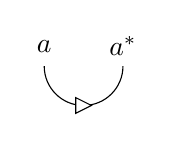
\begin{tikzpicture}[baseline=(current bounding box.center),yscale=-1]
			\draw (0,0) arc (180:0:0.5);
			\draw[fill=white] (0.6,0.5) -- (0.4,0.6) -- (0.4,0.4) -- cycle;
			\node at (0,-0.25) {$a$};
			\node at (1,-0.25) {$a^*$};
		\end{tikzpicture}\ =\kappa_a^*\ 
		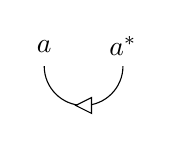
\begin{tikzpicture}[baseline=(current bounding box.center),yscale=-1]
			\draw (0,0) arc (180:0:0.5);
			\draw[fill=white] (0.4,0.5) -- (0.6,0.4) -- (0.6,0.6) -- cycle;
			\node at (0,-0.25) {$a$};
			\node at (1,-0.25) {$a^*$};
		\end{tikzpicture}
	\end{align}
The cups and caps with left-directed flags are related to those with right-directed flags via the factor $\kappa_a$ (or $\kappa_a^*$, respectively). These cups and caps are already familiar to us as evaluation\index{evaluation} and coevaluation\index{coevaluation} morphisms. They appeared when we introduced left and right duals of objects in \cref{sec:fusioncat}. Using this notation, we can rewrite \cref{eq:FrobSchur} as
	\begin{equation}
		\begin{tikzpicture}[baseline=(current bounding box.center)]
			\draw (0,0) arc (180:0:0.5);
			\draw[fill=white] (0.6,0.5) -- (0.4,0.6) -- (0.4,0.4) -- cycle;
			\draw (0,0) arc (0:-180:0.5);
			\draw[fill=white] (-0.4,-0.5) -- (-0.6,-0.6) -- (-0.6,-0.4) -- cycle;
			\node at (-0.2,0.25) {$a^*$};
			\node at (1,-0.25) {$a$};
			\node at (-1,0.25) {$a$};
		\end{tikzpicture}=\kappa_a\ 
		\begin{tikzpicture}[baseline=(current bounding box.center)]
			\draw (0,-0.75) to node[right] {$a$} (0,0.75);
		\end{tikzpicture}.
	\end{equation}
To ensure isotopy invariance when bending lines vertically, one needs to pair up cups and caps with opposing flags since the factors cancel out in this case:
	\begin{equation}
		\begin{tikzpicture}[baseline=(current bounding box.center)]
			\draw (0,0) arc (180:0:0.5);
			\draw[fill=white] (0.4,0.5) -- (0.6,0.4) -- (0.6,0.6) -- cycle;
			\draw (0,0) arc (0:-180:0.5);
			\draw[fill=white] (-0.4,-0.5) -- (-0.6,-0.6) -- (-0.6,-0.4) -- cycle;
			\node at (-0.2,0.25) {$a^*$};
			\node at (1,-0.25) {$a$};
			\node at (-1,0.25) {$a$};
		\end{tikzpicture}=\ 
		\begin{tikzpicture}[baseline=(current bounding box.center)]
			\draw (0,-0.75) to node[right] {$a$} (0,0.75);
		\end{tikzpicture}=
		\begin{tikzpicture}[baseline=(current bounding box.center),yscale=-1]
			\draw (0,0) arc (180:0:0.5);
			\draw[fill=white] (0.4,0.5) -- (0.6,0.4) -- (0.6,0.6) -- cycle;
			\draw (0,0) arc (0:-180:0.5);
			\draw[fill=white] (-0.4,-0.5) -- (-0.6,-0.6) -- (-0.6,-0.4) -- cycle;
			\node at (0.2,-0.25) {$a^*$};
			\node at (1,-0.25) {$a$};
			\node at (-1,0.25) {$a$};
		\end{tikzpicture}.
	\end{equation}
There are analogous identities for $a^*$:
	\begin{equation}
		\begin{tikzpicture}[baseline=(current bounding box.center)]
			\draw (0,0) arc (180:0:0.5);
			\draw[fill=white] (0.6,0.5) -- (0.4,0.4) -- (0.4,0.6) -- cycle;
			\draw (0,0) arc (0:-180:0.5);
			\draw[fill=white] (-0.6,-0.5) -- (-0.4,-0.6) -- (-0.4,-0.4) -- cycle;
			\node at (-0.2,0.25) {$a$};
			\node at (1,-0.25) {$a^*$};
			\node at (-1,0.25) {$a^*$};
		\end{tikzpicture}=\ 
		\begin{tikzpicture}[baseline=(current bounding box.center)]
			\draw (0,-0.75) to node[right] {$a^*$} (0,0.75);
		\end{tikzpicture}=
		\begin{tikzpicture}[baseline=(current bounding box.center),yscale=-1]
			\draw (0,0) arc (180:0:0.5);
			\draw[fill=white] (0.6,0.5) -- (0.4,0.4) -- (0.4,0.6) -- cycle;
			\draw (0,0) arc (0:-180:0.5);
			\draw[fill=white] (-0.6,-0.5) -- (-0.4,-0.6) -- (-0.4,-0.4) -- cycle;
			\node at (0.2,-0.25) {$a$};
			\node at (1,-0.25) {$a^*$};
			\node at (-1,0.25) {$a^*$};
		\end{tikzpicture}.
	\end{equation}
Whenever cups and caps are paired up with opposing flags so that the factor cancels out, the flags can be left implicit. This is the convention that we will use from now on and in most cases, the flags are paired up properly so they usually do not show up explicitly.

By defining the same kind of vectors for $a^*$ instead of $a$ and exploiting their relations, one can find several useful identities for the quantum dimension $d_a$ and the factor $\kappa_a$ (see \cite[App.\ E]{kitaev_anyons_2006}):
	\begin{align}
		d_a=d_{a^*},\hspace{20pt}\kappa_{a^*}=\kappa_a^*,\hspace{20pt}|\kappa_a|=1.
	\end{align}
Using this notation and \cref{eq:bigon2}, we can express the quantum dimension of a particle $a$ as 	
	\begin{equation}
	\label{eq:qdimgraph}
		\begin{tikzpicture}[baseline=(current bounding box.center)]
			\draw (0,0) circle (0.5cm);
			\node at (0.75,0) {$a^*$};
			\node at (-0.75,0) {$a$};
			\draw[fill=white] (0.1,0.5) -- (-0.1,0.4) -- (-0.1,0.6) -- cycle;
			\draw[fill=white] (0.1,-0.5) -- (-0.1,-0.4) -- (-0.1,-0.6) -- cycle;
		\end{tikzpicture}=
		\begin{tikzpicture}[baseline=(current bounding box.center)]
			\draw (0,0) circle (0.5cm);
			\node at (-0.75,0) {$a$};
		\end{tikzpicture}
		=d_a.
	\end{equation}

These cups and caps can also be used to bend lines down, for example if you want to rotate a splitting vertex into a fusion vertex. Analogously, we can bend lines up to rotate a fusion vertex to become a splitting vertex. The four possible cases are
	\begin{align}
		\begin{tikzpicture}[baseline=(current bounding box.center),xscale=-1]
			\draw (0,1) -- (0.5,0.5) -- (1,1) -- (1.5,0.5) -- (1.5,0);
			\draw[dashed] (1,1) -- (1,1.5);
			\node at (1,1.75) {$\mathbf{1}$};
			\draw (0.5,0.5) -- (0.5,0);
			\node at (0,1.25) {$b$};
			\node at (0.7,1) {$a$};
			\node at (1.5,-0.25) {$a^*$};
			\node at (0.5,-0.25) {$c$};
		\end{tikzpicture}&=
		\begin{tikzpicture}[baseline=(current bounding box.center),xscale=-1]
			\draw (0,1) -- (0.5,0.5) -- (1,1);
			\draw (0.5,0.5) -- (0.5,0);
			\node at (0,1.25) {$b$};
			\node at (1,1.25) {$a$};
			\node at (1.85,-0.25) {$a^*$};
			\node at (0.5,-0.25) {$c$};
			\draw (1,1) arc (135:0:0.5);
			\draw (1.85,0.65) -- (1.85,0);
			\draw[fill=white] (1.475,1.14) -- (1.275,1.04) -- (1.275,1.24) -- cycle;
		\end{tikzpicture}=A_c^{ab}
		\begin{tikzpicture}[baseline=(current bounding box.center),xscale=-1]
			\draw (0,0) -- (0.5,0.5) -- (1,0);
			\draw (0.5,0.5) -- (0.5,1);
			\node at (0,-0.25) {$c$};
			\node at (0.5,1.25) {$b$};
			\node at (1,-0.25) {$a^*$};
		\end{tikzpicture}\\
		\begin{tikzpicture}[baseline=(current bounding box.center),xscale=-1,yscale=-1]
			\draw (0,1) -- (0.5,0.5) -- (1,1) -- (1.5,0.5) -- (1.5,0);
			\draw[dashed] (1,1) -- (1,1.5);
			\node at (1,1.75) {$\mathbf{1}$};
			\draw (0.5,0.5) -- (0.5,0);
			\node at (0,1.25) {$b$};
			\node at (0.7,1) {$a$};
			\node at (1.5,-0.25) {$a^*$};
			\node at (0.5,-0.25) {$c$};
		\end{tikzpicture}&=
		\begin{tikzpicture}[baseline=(current bounding box.center),xscale=-1,yscale=-1]
			\draw (0,1) -- (0.5,0.5) -- (1,1);
			\draw (0.5,0.5) -- (0.5,0);
			\node at (0,1.25) {$b$};
			\node at (1,1.25) {$a$};
			\node at (1.85,-0.25) {$a^*$};
			\node at (0.5,-0.25) {$c$};
			\draw (1,1) arc (135:0:0.5);
			\draw (1.85,0.65) -- (1.85,0);
			\draw[fill=white] (1.475,1.14) -- (1.275,1.04) -- (1.275,1.24) -- cycle;
		\end{tikzpicture}=A^c_{ab}
		\begin{tikzpicture}[baseline=(current bounding box.center),xscale=-1,yscale=-1]
			\draw (0,0) -- (0.5,0.5) -- (1,0);
			\draw (0.5,0.5) -- (0.5,1);
			\node at (0,-0.25) {$c$};
			\node at (0.5,1.25) {$b$};
			\node at (1,-0.25) {$a^*$};
		\end{tikzpicture}\\
		\begin{tikzpicture}[baseline=(current bounding box.center)]
			\draw (0,1) -- (0.5,0.5) -- (1,1) -- (1.5,0.5) -- (1.5,0);
			\draw[dashed] (1,1) -- (1,1.5);
			\node at (1,1.75) {$\mathbf{1}$};
			\draw (0.5,0.5) -- (0.5,0);
			\node at (0,1.25) {$a$};
			\node at (0.7,1) {$b$};
			\node at (1.5,-0.25) {$b^*$};
			\node at (0.5,-0.25) {$c$};
		\end{tikzpicture}&=
		\begin{tikzpicture}[baseline=(current bounding box.center)]
			\draw (0,1) -- (0.5,0.5) -- (1,1);
			\draw (0.5,0.5) -- (0.5,0);
			\node at (0,1.25) {$a$};
			\node at (1,1.25) {$b$};
			\node at (1.85,-0.25) {$b^*$};
			\node at (0.5,-0.25) {$c$};
			\draw (1,1) arc (135:0:0.5);
			\draw (1.85,0.65) -- (1.85,0);
			\draw[fill=white] (1.475,1.14) -- (1.275,1.04) -- (1.275,1.24) -- cycle;
		\end{tikzpicture}=B_c^{ab}
		\begin{tikzpicture}[baseline=(current bounding box.center)]
			\draw (0,0) -- (0.5,0.5) -- (1,0);
			\draw (0.5,0.5) -- (0.5,1);
			\node at (0,-0.25) {$c$};
			\node at (0.5,1.25) {$a$};
			\node at (1,-0.25) {$b^*$};
		\end{tikzpicture}\\
		\begin{tikzpicture}[baseline=(current bounding box.center),yscale=-1]
			\draw (0,1) -- (0.5,0.5) -- (1,1) -- (1.5,0.5) -- (1.5,0);
			\draw[dashed] (1,1) -- (1,1.5);
			\node at (1,1.75) {$\mathbf{1}$};
			\draw (0.5,0.5) -- (0.5,0);
			\node at (0,1.25) {$a$};
			\node at (0.7,1) {$b$};
			\node at (1.5,-0.25) {$b^*$};
			\node at (0.5,-0.25) {$c$};
		\end{tikzpicture}&=
		\begin{tikzpicture}[baseline=(current bounding box.center),yscale=-1]
			\draw (0,1) -- (0.5,0.5) -- (1,1);
			\draw (0.5,0.5) -- (0.5,0);
			\node at (0,1.25) {$a$};
			\node at (1,1.25) {$b$};
			\node at (1.85,-0.25) {$b^*$};
			\node at (0.5,-0.25) {$c$};
			\draw (1,1) arc (135:0:0.5);
			\draw (1.85,0.65) -- (1.85,0);
			\draw[fill=white] (1.475,1.14) -- (1.275,1.04) -- (1.275,1.24) -- cycle;
		\end{tikzpicture}=B^c_{ab}
		\begin{tikzpicture}[baseline=(current bounding box.center),yscale=-1]
			\draw (0,0) -- (0.5,0.5) -- (1,0);
			\draw (0.5,0.5) -- (0.5,1);
			\node at (0,-0.25) {$c$};
			\node at (0.5,1.25) {$a$};
			\node at (1,-0.25) {$b^*$};
		\end{tikzpicture},
	\end{align}
where
	\begin{align}
		A_c^{ab}&=\sqrt{\frac{d_a d_b}{d_c}}\overline{\left(F_b^{a^*a b}\right)}_{c\mathbf{1}} \label{eq:A}\\
		A_{ab}^c&=\overline{A_c^{ab}} \label{eq:As}\\
		B_c^{ab}&=\sqrt{\frac{d_a d_b}{d_c}}\left(F_a^{a b b^*}\right)_{\mathbf{1}c} \label{eq:B}\\
		B_{ab}^c&=\overline{B_c^{ab}}.\label{eq:Bs}
	\end{align}
These formulas are derived by exploiting the completeness relation \cref{eq:identity}. We show how this works by performing the computation of $B_c^{ab}$ step-by-step:
	\begin{align}
		\begin{tikzpicture}[baseline=(current bounding box.center)]
			\draw (0,1) -- (0.5,0.5) -- (1,1) -- (1.5,0.5) -- (1.5,0);
			\draw[dashed] (1,1) -- (1,1.5);
			\node at (1,1.75) {\small $\mathbf{1}$};
			\draw (0.5,0.5) -- (0.5,0);
			\node at (0,1.25) {\small $a$};
			\node at (0.7,1) {\small $b$};
			\node at (1.5,-0.25) {\small $b^*$};
			\node at (0.5,-0.25) {\small $c$};
		\end{tikzpicture}&=\sum_{a'}\sqrt{\frac{d_{a'}}{d_b d_c}}
		\begin{tikzpicture}[baseline=(current bounding box.center)]
			\draw (0,1) -- (0.5,0.5) -- (1,1) -- (1.5,0.5) -- (1.5,0);
			\draw (0.5,0) -- (1,-0.5) -- (1.5,0);
			\draw (1,-0.5) to node[left] {\small $a'$} (1,-1);
			\draw (0.5,-1.5) -- (1,-1) -- (1.5,-1.5);
			\draw[dashed] (1,1) -- (1,1.5);
			\node at (1,1.75) {\small $\mathbf{1}$};
			\draw (0.5,0.5) -- (0.5,0);
			\node at (0,1.25) {\small $a$};
			\node at (0.7,1) {\small $b$};
			\node at (1.65,-0.25) {\small $b^*$};
			\node at (0.35,-0.25) {\small $c$};
			\node at (1.65,-1.7) {\small $b^*$};
			\node at (0.35,-1.7) {\small $c$};
		\end{tikzpicture}\\
		&=\sum_{a',c'}\sqrt{\frac{d_{a'}}{d_b d_c}}\left(F_{a'}^{abb^*}\right)_{c'c}
		\begin{tikzpicture}[baseline=(current bounding box.center)]
			\draw (0.5,0) -- (1,-0.5) -- (1.5,0);
			\draw (1.25,-0.25) -- (1,0);
			\draw (1,0) to node[left] {\small $b$} (1,0.25);
			\draw (1,0.25) -- (1.25,0.5);
			\draw (1.5,0) to node[right] {\small $b^*$} (1.5,0.25);
			\draw (1.5,0.25) -- (1.25,0.5);
			\draw[dashed] (1.25,0.5) -- (1.25,0.75);
			\node at (1.25,1) {\small $\mathbf{1}$};
			\draw (1,-0.5) to node[left] {\small $a'$} (1,-1);
			\draw (0.5,-1.5) -- (1,-1) -- (1.5,-1.5);
			\draw (0.5,0.75) -- (0.5,0);
			\node at (1.35,-0.45) {\small $c'$};
			\node at (0.3,0.5) {\small $a$};
			\node at (1.65,-1.7) {\small $b^*$};
			\node at (0.35,-1.7) {\small $c$};
		\end{tikzpicture}\\
		&=\sum_{a',c'}\sqrt{\frac{d_{a'}}{d_b d_c}}\left(F_{a'}^{abb^*}\right)_{c'c}\sqrt{\frac{d_\mathbf{1}}{d_bd_{b^*}}}\ \delta_{c',\mathbf{1}}
		\begin{tikzpicture}[baseline=(current bounding box.center)]
			\draw (0,0) to node[right] {$a'$} (0,0.5);
			\draw (-0.5,-0.5) -- (0,0);
			\draw (0.5,-0.5) -- (0,0);
			\draw (0,0.5) -- (-0.5,1);
			\draw[dashed] (0,0.5) -- (0.5,1);
			\node at (-0.5,1.25) {$a$};
			\node at (0.5,1.25) {$\mathbf{1}$};
			\node at (-0.5,-0.75) {$c$};
			\node at (0.5,-0.75) {$b^*$};
		\end{tikzpicture}\\
		&=\sqrt{\frac{d_ad_b}{d_c}}\left(F_a^{abb^*}\right)_{\mathbf{1}c}
		\begin{tikzpicture}[baseline=(current bounding box.center)]
			\draw (0,0) -- (0,0.5);
			\draw (-0.5,-0.5) -- (0,0);
			\draw (0.5,-0.5) -- (0,0);
			\node at (0,0.75) {$a$};
			\node at (-0.5,-0.75) {$c$};
			\node at (0.5,-0.75) {$b^*$};
		\end{tikzpicture},
	\end{align}
where in the last step we have used the fact that $d_b=d_{b^*}$ and that $N_{a\mathbf{1}}^{a'}=\delta_{a,a'}$. The derivations of the other operators use the same techniques. The operators $A_c^{ab}$ and $B_c^{ab}$ are unitary (see \cite[Thm.\ E.6]{kitaev_anyons_2006}), which implies the following identities:	
	\begin{equation}
	\label{eq:Nidentities}
		N_{ab}^c=N_{a^*c}^b=N_{b c^*}^{a^*}=N_{b^*a^*}^{c^*}=N_{c^*a}^{b^*}=N_{cb^*}^a.
	\end{equation}
From the unitarity of these operators we can directly derive the following identities for F-matrices:
	\begin{align}
		\left|\left(F_b^{a^*ab}\right)_{c\mathbf{1}}\right|^2&=\frac{d_c}{d_a d_b},\\
		\left|\left(F_a^{abb^*}\right)_{\mathbf{1}c}\right|^2&=\frac{d_c}{d_a d_b}.\label{eq:Fidentities}
	\end{align}
Furthermore, the fact that the $F$-matrices themselves are unitary matrices implies
	\begin{equation}
	\label{eq:Funitary}
		\left|\left(F_u^{abc}\right)_{ef}\right|^2=1,
	\end{equation}
whenever $e$ and $f$ are the \emph{unique} labels allowed by the fusion rules for $u,a,b,c$, since in this case the $F$-move is a unitary map between one-dimensional vector spaces.

Additionally, we can use the operators $A$ and $B$ to prove an important identity of the quantum dimensions of anyonic particles: 
\begin{thm}
	\label{thm:qdimrelation}
	The quantum dimension\index{quantum dimension} fulfils the key identity
	\begin{equation}
	d_a d_b=\sum_c N_{ab}^c d_c.
	\end{equation}
\end{thm}
\begin{proof}
	This can be shown via the following calculation:
		\begin{align}
			d_a d_b&=\begin{tikzpicture}[scale=0.6,baseline=(current bounding box.center)]
				\draw (0,0) circle (0.5cm);
				\draw (0,0) circle (1cm);
				\node at (-0.25,0) {\small $a$};
				\node at (-1.25,0) {\small $b$};
			\end{tikzpicture}\\
			&=\sum_cN_{ab}^c\sqrt{\frac{d_c}{d_ad_b}}\ \begin{tikzpicture}[scale=0.7,baseline=(current bounding box.center)]
				\draw (0,0) to node[left] {\small $c$} (0,0.5);
				\draw (0,0.5) -- (0.5,1);	
				\draw (0,0.5) -- (-0.5,1);
				\draw (0,0) -- (-0.5,-0.5);
				\draw (0,0) -- (0.5,-0.5);
				\draw (0.5,1) arc (135:0:0.5cm);
				\draw (-0.5,1) arc (225:180:0.5cm);
				\begin{scope}[yscale=-1]
					\draw (0.5,0.5) arc (135:0:0.5cm);
					\draw (-0.5,0.5) arc (225:180:0.5cm);
					\draw (-0.645,0.85) to[bend left=90] (2,0.85);
				\end{scope}
				\draw (1.355,0.65) to node[right] {\small $a^*$} (1.355,-0.15);
				\draw (-0.645,1.35) to[bend left=90] (2,1.35);
				\draw (2,1.35) to node[right] {\small $b^*$} (2,-0.85);
				\node at (-0.75,1) {\small $b$};
				\node at (-0.75,-0.5) {\small $b$};
				\node at (0.55,0.65) {\small $a$};
				\node at (0.55,-0.15) {\small $a$};
			\end{tikzpicture}\\
			&=\sum_cN_{ab}^c\sqrt{\frac{d_c}{d_ad_b}}B_c^{ba}B_{ba}^c\ \begin{tikzpicture}[scale=0.7,baseline=(current bounding box.center)]
				\draw (0,0) to[bend left=70] node[left] {\small $c$} (0,1);
				\draw (0,0) to[bend right=70] node[right] {\small $a^*$} (0,1);
				\draw (0,0) to node [left, near end] {\small $b$} (0,-0.25);
				\draw (0,1) to node [left, near end] {\small $b$} (0,1.25);
				\draw (0,1.25) arc (180:0:0.5);
				\draw (0,-0.25) arc (-180:0:0.5);
				\draw (1,-0.25) to node[right] {\small $b^*$} (1,1.25);
			\end{tikzpicture}\\
			&=\sum_cN_{ab}^c\sqrt{\frac{d_c}{d_ad_b}}B_c^{ba}B_{ba}^cA_{ca^*}^bA_b^{ca^*}\ \begin{tikzpicture}[xscale=0.6,yscale=0.7,baseline=(current bounding box.center)]
				\draw (0,0) to node[left] {\small $a^*$} (0,0.5);
				\draw (0,0.5) -- (0.5,1);
				\draw (0,0.5) -- (-0.5,1);
				\draw (0,0) -- (0.5,-0.5);
				\draw (0,0) -- (-0.5,-0.5);
				\draw (0.5,1) arc (135:0:0.5cm);
				\draw (0.5,-0.5) arc (-135:0:0.5cm);
				\draw (1.355,0.65) to node[right] {\small $b^*$} (1.355,-0.15);
				\begin{scope}[xscale=-1]
					\draw (0.5,1) arc (135:0:0.5cm);
					\draw (0.5,-0.5) arc (-135:0:0.5cm);
					\draw (1.355,0.65) to node[left] {\small $c$} (1.355,-0.15);
				\end{scope}
			\end{tikzpicture}\\
			&=\sum_cN_{ab}^c\sqrt{\frac{d_c}{d_ad_b}}B_c^{ba}B_{ba}^cA_{ca^*}^bA_b^{ca^*}B_{a^*}^{c^*b}B_{c^*b}^{a^*}\ \begin{tikzpicture}[scale=0.7,baseline=(current bounding box.center)]
				\begin{scope}[xscale=-1]
					\draw (0,0) to[bend left=70] node[right] {\small $b^*$} (0,1);
					\draw (0,0) to[bend right=70] node[left] {\small $a^*$} (0,1);
					\draw (0,0) to node [right, near end] {\small $c^*$} (0,-0.25);
					\draw (0,1) to node [right, near end] {\small $c^*$} (0,1.25);
					\draw (0,1.25) arc (180:0:0.5);
					\draw (0,-0.25) arc (-180:0:0.5);
					\draw (1,-0.25) to node[left] {\small $c$} (1,1.25);
				\end{scope}
			\end{tikzpicture}\\
			&=\sum_cN_{ab}^c\sqrt{\frac{d_c}{d_ad_b}}B_c^{ba}B_{ba}^cA_{ca^*}^bA_b^{ca^*}B_{a^*}^{c^*b}B_{c^*b}^{a^*}\sqrt{\frac{d_{a^*}d_{b^*}}{d_{c^*}}}\ 
			\begin{tikzpicture}[scale=0.7,baseline=(current bounding box.center)]
				\draw (0,0) circle (0.5cm);
				\node at (-0.75,0) {\small $c$};
			\end{tikzpicture}\\
			&=\sum_cN_{ab}^cB_c^{ba}\overline{B^{ba}_c}\overline{A^{ca^*}_b} A_b^{ca^*}B_{a^*}^{c^*b}\overline{B^{c^*b}_{a^*}} d_c\\
			&=\sum_cN_{ab}^c d_c,
		\end{align}
	where the last equality follows from the fact that the operators $A_c^{ab}$ and $B_c^{ab}$ are unitary.
\end{proof}

Another important notion we have to define is the trace of an operator. Similar to the categorical definition of trace given in \cref{def:trace} and \cref{rem:trace}, we take the trace of a diagram by closing it with loops that connect the outgoing lines with the respective incoming lines at the same position. For instance, consider an operator $X$ that maps $n$ incoming particles $a_1,a_2,\dots,a_n$ to $n$ outgoing particles $a_1',a_2',\dots,a_n'$. We can represent this graphically as
	\begin{equation}
		\begin{tikzpicture}[scale=0.7,baseline=(current bounding box.center)]
			\draw (0,0) rectangle (2.5,1.5);
			\node at (1.25,0.75) {$X$};
			\draw (0.25,-0.75) -- (0.25,0);
			\draw (0.75,-0.75) -- (0.75,0);
			\draw (2.25,-0.75) -- (2.25,0);
			\node at (1.5,-0.375) {$\dots$};
			\draw (0.25,2.25) -- (0.25,1.5);
			\draw (0.75,2.25) -- (0.75,1.5);
			\draw (2.25,2.25) -- (2.25,1.5);
			\node at (1.5,1.875) {$\dots$};
			\node at (0.25,-1.1) {\small $a_1$};
			\node at (0.75,-1.1) {\small $a_2$};
			\node at (2.25,-1.1) {\small $a_n$};
			\node at (0.25,2.6) {\small $a'_1$};
			\node at (0.75,2.6) {\small $a'_2$};
			\node at (2.25,2.6) {\small $a'_n$};
		\end{tikzpicture}\ .
	\end{equation}
To calculate the trace\index{trace} of $X$ we connect every outgoing leg with the corresponding ingoing leg:
	\begin{equation}
	\Tr(X)=
		\begin{tikzpicture}[scale=0.7,baseline=(current bounding box.center)]
			\draw (0,0) rectangle (2.5,1.5);
			\node at (1.25,0.75) {$X$};
%			\draw (0.25,-0.75) -- (0.25,0);
%			\draw (0.75,-0.75) -- (0.75,0);
			\draw (2.25,-0.75) -- (2.25,0);
			\node at (1.5,-0.375) {$\dots$};
%			\draw (0.25,2.25) -- (0.25,1.5);
%			\draw (0.75,2.25) -- (0.75,1.5);
			\draw (2.25,2.25) -- (2.25,1.5);
			\node at (1.5,1.875) {$\dots$};
			\node at (-0.1,-0.85) {\small $a_1$};
%			\node at (0.75,-1.1) {\small $a_2$};
			\node at (1.9,-0.85) {\small $a_n$};
			\node at (-0.1,2.35) {\small $a'_1$};
%			\node at (0.75,2.6) {\small $a'_2$};
			\node at (1.9,2.35) {\small $a'_n$};
			\draw (2.25,2.25) arc (180:0:0.5cm);
			\draw (2.25,-0.75) arc (-180:0:0.5cm);
			\draw (3.25,2.25) -- (3.25,-0.75);
			\node at (4,0.75) {$\dots$};
			\draw[rounded corners=7mm] (0.75,1.5) -- (0.75,3) -- (4.75,3) -- (4.75,-1.5) -- (0.75,-1.5) -- (0.75,0);
			\draw[rounded corners=9mm] (0.25,1.5) -- (0.25,3.5) -- (5.25,3.5) -- (5.25,-2) -- (0.25,-2) -- (0.25,0);
		\end{tikzpicture}\ .
	\end{equation}
	


\subsection*{Exchange properties.}

Apart from fusing or splitting anyons it is also possible to \emph{braid} them. As we have seen above, the statistics of an anyon model is manifested in the evolution of the wave function of a system when two particles are exchanged\index{braiding}. In two spatial dimensions particles are allowed to exhibit any statistical behaviour as the restrictions that hold in three dimensions do not apply to two-dimensional systems.

When exchanging two particles $a$ and $b$ in the plane, there are two possible ways to do this which are topologically inequivalent:
	\begin{equation}
		\begin{tikzpicture}[scale=0.8]
			\node at (1,-0.25) {$a$};
			\node at (2,-0.25) {$b$};
			\node at (1,1.75) {$b$};
			\node at (2,1.75) {$a$};
			\begin{knot}[consider self intersections=true,ignore endpoint intersections=false]
			\strand (1,0)to[out=90,in=270](2,1.5);
			\strand (2,0)to[out=90,in=270](1,1.5);
			\end{knot}
		\end{tikzpicture}\hspace{50pt}
		\begin{tikzpicture}[scale=0.8]
			\node at (1,-0.25) {$a$};
			\node at (2,-0.25) {$b$};
			\node at (1,1.75) {$b$};
			\node at (2,1.75) {$a$};
			\begin{knot}[consider self intersections=true,ignore endpoint intersections=false]
			\strand (2,0)to[out=90,in=270](1,1.5);
			\strand (1,0)to[out=90,in=270](2,1.5);
			\end{knot}
		\end{tikzpicture}
	\end{equation}
We refer to the left diagram as right-handed braiding, denoted $R_{ab}$, and to the right diagram as left-handed braiding, denoted $R_{ab}^{-1}$. This is analogous to the braiding in the categorical sense as defined in \cref{def:braiding}.

To describe the braiding operator, consider the vector space $V_c^{ab}$ of a particle $c$ splitting into two particles $a$ and $b$. Suppose this vector space is one-dimensional and let $e_c^{ab}$ be its basis vector in terms of fusion trees. When the particles $a$ and $b$ are braided by $R_{ab}$, the vector $e_c^{ab}$ in $V_c^{ab}$ is transformed into a vector $R_{ab}e_c^{ab}$ in the vector space $V_c^{ba}$. The vector space $V_c^{ba}$ also has a corresponding basis vector $e_c^{ba}$. Since both state, $R_{ab}e_c^{ab}$ and $e_c^{ba}$, are non-zero vectors in the one-dimensional vector space $V_c^{ba}$, they are equal up to a phase. This phase is denoted $R_c^{ab}$, i.e., $R_{ab}e_c^{ab}=R_c^{ab}e_c^{ba}$:
	\begin{equation}
	\label{eq:braiding}
		R_{ab}
		\begin{tikzpicture}[scale=0.8,baseline=(current bounding box.center)]
			\node at (1.5,-1.25) {$c$}; 
			\node at (1,1.3) {$a$};
			\node at (2,1.3) {$b$};
			\draw (1.5,-1) -- (1.5,-0.25);
			\draw (1.5,-0.25) to [bend left=15] (1,1.05);
			\draw (1.5,-0.25) to [bend right=15] (2,1.05);
		\end{tikzpicture}\ =\ 
		\begin{tikzpicture}[xscale=0.8,yscale=0.8,baseline=(current bounding box.center)]
			\node at (1.5,-1.25) {$c$}; 
			\node at (1,1.3) {$b$};
			\node at (2,1.3) {$a$};
			\draw (1.5,-1) -- (1.5,-0.5);
			\draw (1.5,-0.5) -- (1,0);
			\draw (1.5,-0.5) -- (2,0);
			\begin{knot}[consider self intersections=true,ignore endpoint intersections=false,yscale=0.7]
			\strand (1,0)to[out=120,in=270](2,1.5);
			\strand (2,0)to[out=60,in=270](1,1.5);
			\end{knot}
		\end{tikzpicture}
		\ =\ R_c^{ab}\begin{tikzpicture}[scale=0.8,baseline=(current bounding box.center)]
			\node at (1.5,-1.25) {$c$}; 
			\node at (1,1.3) {$b$};
			\node at (2,1.3) {$a$};
			\draw (1.5,-1) -- (1.5,-0.25);
			\draw (1.5,-0.25) to [bend left=15] (1,1.05);
			\draw (1.5,-0.25) to [bend right=15] (2,1.05);
		\end{tikzpicture}.
	\end{equation}	
From this relation, we can show that 
	\begin{equation}
		\begin{tikzpicture}[scale=0.8,baseline=(current bounding box.center)]
			\node at (1.5,-1.25) {$c$}; 
			\node at (1,1.3) {$a$};
			\node at (2,1.3) {$b$};
			\draw (1.5,-1) -- (1.5,-0.25);
			\draw (1.5,-0.25) to [bend left=15] (1,1.05);
			\draw (1.5,-0.25) to [bend right=15] (2,1.05);
		\end{tikzpicture}=
		\begin{tikzpicture}[xscale=0.8,yscale=0.8,baseline=(current bounding box.center)]
			\node at (1.5,-1.25) {$c$}; 
			\node at (1,2.5) {$a$};
			\node at (2,2.5) {$b$};
			\draw (1.5,-1) -- (1.5,-0.5);
			\draw (1.5,-0.5) -- (1,0);
			\draw (1.5,-0.5) -- (2,0);
			\begin{knot}[consider self intersections=true,ignore endpoint intersections=false,yscale=0.7]
			\strand (1,0)to[out=120,in=270](2,1.5)to[out=90,in=270](1,3);
			\strand (2,0)to[out=60,in=270](1,1.5)to[out=90,in=270](2,3);
			\draw[dashed] (0.75,1.5) -- (2.25,1.5);
			\end{knot}
		\end{tikzpicture}=R_c^{ab}\ 
		\begin{tikzpicture}[xscale=0.8,yscale=0.8,baseline=(current bounding box.center)]
			\node at (1.5,-1.25) {$c$}; 
			\node at (1,2.5) {$a$};
			\node at (2,2.5) {$b$};
			\draw (1.5,-1) -- (1.5,-0.25);
			\draw (1.5,-0.25) to [bend left=15] (1,1.05);
			\draw (1.5,-0.25) to [bend right=15] (2,1.05);
			\begin{knot}[consider self intersections=true,ignore endpoint intersections=false,yscale=0.7]
			\strand (2,1.5)to[out=90,in=270](1,3);
			\strand (1,1.5)to[out=90,in=270](2,3);
			\draw[dashed] (0.75,1.5) -- (2.25,1.5);
			\end{knot}
		\end{tikzpicture}
	\end{equation}
which tells us about the action of $R_{ab}^{-1}$:
	\begin{equation}
		R_{ab}^{-1}
		\begin{tikzpicture}[scale=0.8,baseline=(current bounding box.center)]
		\node at (1.5,-1.25) {$c$}; 
		\node at (1,1.3) {$b$};
		\node at (2,1.3) {$a$};
		\draw (1.5,-1) -- (1.5,-0.25);
		\draw (1.5,-0.25) to [bend left=15] (1,1.05);
		\draw (1.5,-0.25) to [bend right=15] (2,1.05);
		\end{tikzpicture}\ =\ 
		\begin{tikzpicture}[xscale=0.8,yscale=0.8,baseline=(current bounding box.center)]
			\node at (1.5,-1.25) {$c$}; 
			\node at (1,1.3) {$a$};
			\node at (2,1.3) {$b$};
			\draw (1.5,-1) -- (1.5,-0.5);
			\draw (1.5,-0.5) -- (1,0);
			\draw (1.5,-0.5) -- (2,0);
			\begin{knot}[consider self intersections=true,ignore endpoint intersections=false,yscale=0.7]
			\strand (2,0)to[out=60,in=270](1,1.5);
			\strand (1,0)to[out=120,in=270](2,1.5);
			\end{knot}
		\end{tikzpicture}
		\ =\ \left(R_c^{ab}\right)^{-1}
		\begin{tikzpicture}[scale=0.8,baseline=(current bounding box.center)]
			\node at (1.5,-1.25) {$c$}; 
			\node at (1,1.3) {$a$};
			\node at (2,1.3) {$b$};
			\draw (1.5,-1) -- (1.5,-0.25);
			\draw (1.5,-0.25) to [bend left=15] (1,1.05);
			\draw (1.5,-0.25) to [bend right=15] (2,1.05);
		\end{tikzpicture}.
	\end{equation}
Hence, we have two ways of braiding two anyons around each other. Here, $R_c^{ab}$ is a phase factor because the corresponding vector spaces are one-dimensional in the multiplicity-free case. In general, the vector spaces can be higher dimensional, in which case it is a unitary matrix called the $R$-matrix\index{R-matrix@$R$-matrix}. Equation \cref{eq:braiding} then is of the form
	\begin{equation}
		R_{ab}
		\begin{tikzpicture}[scale=0.8,baseline=(current bounding box.center)]
		\node at (1.5,-1.25) {$c$}; 
		\node at (1,1.3) {$a$};
		\node at (2,1.3) {$b$};
		\node at (1.75,-0.25) {$\ \mu$};
		\draw (1.5,-1) -- (1.5,-0.25);
		\draw (1.5,-0.25) to [bend left=15] (1,1.05);
		\draw (1.5,-0.25) to [bend right=15] (2,1.05);
		\end{tikzpicture}\ =\ 
		\begin{tikzpicture}[xscale=0.8,yscale=0.8,baseline=(current bounding box.center)]
		\node at (1.5,-1.25) {$c$}; 
		\node at (1,1.3) {$b$};
		\node at (2,1.3) {$a$};
		\node at (1.75,-0.5) {$\ \mu$};
		\draw (1.5,-1) -- (1.5,-0.5);
		\draw (1.5,-0.5) -- (1,0);
		\draw (1.5,-0.5) -- (2,0);
		\begin{knot}[consider self intersections=true,ignore endpoint intersections=false,yscale=0.7]
		\strand (1,0)to[out=120,in=270](2,1.5);
		\strand (2,0)to[out=60,in=270](1,1.5);
		\end{knot}
		\end{tikzpicture}
		\ =\sum_{\nu} \left(R_c^{ab}\right)_{\nu\mu}\begin{tikzpicture}[scale=0.8,baseline=(current bounding box.center)]
		\node at (1.5,-1.25) {$c$}; 
		\node at (1,1.3) {$b$};
		\node at (2,1.3) {$a$};
		\node at (1.75,-0.25) {$\ \nu$};
		\draw (1.5,-1) -- (1.5,-0.25);
		\draw (1.5,-0.25) to [bend left=15] (1,1.05);
		\draw (1.5,-0.25) to [bend right=15] (2,1.05);
		\end{tikzpicture}.
	\end{equation}
Note that unitarity of the $R$-matrix implies that $N_{ab}^c=N_{ba}^c$. It furthermore implies $\left(R_c^{ab}\right)_{\nu\mu}^{-1}=\left(R_c^{ab}\right)_{\nu\mu}^{\dagger}=\overline{\left(R_c^{ba}\right)}_{\mu\nu}$.	

We have to ensure that the braiding operation is compatible with the fusion rules, i.e., $R_{c}^{ba}\neq 0$ if and only if $N_{ab}^c\neq 0$. Additionally, braiding has to be consistent with the $F$-moves. This yields the two so-called \emph{hexagon identities}\index{hexagon equation} that are depicted in \cref{fig:hex}:
%\index{Hexagon equation}
	\begin{align}
	\label{eq:hex}
		R_p^{ca} \left(F_u^{acb}\right)_{pq} R_q^{cb}&=\sum_r \left(F_u^{cab}\right)_{rp} R_u^{cr}\left(F_u^{abc}\right)_{qr}\\
	\label{eq:hex2}
		\left(R_p^{ac}\right)^{-1} \left(F_u^{acb}\right)_{pq} \left(R_q^{bc}\right)^{-1}&=\sum_r \left(F_u^{cab}\right)_{rp} \left(R_u^{rc}\right)^{-1}\left(F_u^{abc}\right)_{qr}
	\end{align}

\begin{exmp}[Fibonacci anyons]
	\label{ex:FibAnyon}
	\index{Fibonacci anyons}
	We have already encountered the Fibonacci category $\mathbf{Fib}$ as a trivalent category in \cref{ex:TrivFib} and numerous times afterwards, for example in \cref{ex:AOFib} and \cref{ex:FibMod}. Here, we study how we can build an anyon model from this category. First, recall that the Fibonacci category has two simple objects, namely $\mathbf{1}$ and $\tau$ and that the fusion rules are given by
		\begin{align}
			\tau\otimes\mathbf{1}&=\mathbf{1}\otimes\tau=\tau\\
			\tau\otimes\tau&=\mathbf{1}+\tau.
		\end{align}
	We can immediately see that the fusion rules are multiplicity-free and, moreover, that the anyon model is non-abelian since $\sum_c N_{\tau\tau}^c=2$ (compare to \cref{eq:nonabelian}). From the fusion rules we can also see that $\tau$ is its own antiparticle (for $\mathbf{1}$ this is always the case). 
	
	\begin{figure}[H]
	\vspace{20pt}
	\begin{tikzpicture}[yscale=1.4,xscale=1.3]
	\node at (0,-0.15) {\small $u$};
	\node at (0,2.15) {\small $b$};
	\node at (-0.5,2.15) {\small $a$};
	\node at (0.5,2.15) {\small $c$};
	\node at (-0.25,0.5) {\small $p$};
	\draw (0,0) -- (0,0.5);
	\draw (0,0.5) -- (-0.25,0.75);
	\draw (0,0.5) -- (0.5,1);
	\draw (-0.25,0.75) -- (-0.5,1);
	\draw (-0.25,0.75) -- (0,1);
	\begin{knot}[consider self intersections=true,ignore endpoint intersections=false]
	\strand (-0.5,1)to[out=135,in=270](0.5,2);
	\strand (0,1)to[out=45,in=270](-0.5,2);
	\strand (0.5,1)to[out=45,in=270](0,2);				
	\end{knot}
	\begin{scope}[yshift=0cm]
	\draw[->,>=stealth] (0.75,1.5) to node[above] {\small $R^{ca}_p\ \ \ $} (1.75,2.5);
	\draw[->,>=stealth] (3.35,3) to node[above] {\small $F_u^{acb}$} (4.65,3);
	\draw[->,>=stealth] (6.25,2.5) to node[above] {\small $\ \ \ R^{cb}_q$} (7.25,1.5);
	\end{scope}
	\begin{scope}[yshift=2cm]
	\draw[->,>=stealth] (0.75,-1.5) to node[below] {\small $F_u^{cab}\ \ \ \ $} (1.75,-2.5);
	\draw[->,>=stealth] (3.35,-3) to node[above] {\small $R^{cr}_u$} (4.65,-3);
	\draw[->,>=stealth] (6.25,-2.5) to node[below] {\small $\ \ \ F_u^{abc}$} (7.25,-1.5);
	\end{scope}
	\begin{scope}[xshift=2.5cm,yshift=2cm]
	\node at (0,-0.15) {\small $u$};
	\node at (0,2.15) {\small $b$};
	\node at (-0.5,2.15) {\small $a$};
	\node at (0.5,2.15) {\small $c$};
	\node at (-0.25,0.5) {\small $p$};
	\draw (0,0) -- (0,0.5);
	\draw (0,0.5) -- (-0.25,0.75);
	\draw (0,0.5) -- (0.5,1);
	\draw (-0.25,0.75) -- (-0.5,1);
	\draw (-0.25,0.75) -- (0,1);
	\begin{knot}[consider self intersections=true,ignore endpoint intersections=false]
	\strand (-0.5,1)to[out=135,in=270](-0.5,2);
	\strand (0,1)to[out=45,in=270](0.5,2);
	\strand (0.5,1)to[out=45,in=270](0,2);				
	\end{knot}
	\end{scope}
	\begin{scope}[xshift=5.5cm,yshift=2cm]
	\node at (0,-0.15) {\small $u$};
	\node at (0,2.15) {\small $b$};
	\node at (-0.5,2.15) {\small $a$};
	\node at (0.5,2.15) {\small $c$};
	\node at (0.25,0.5) {\small $q$};
	\draw (0,0) -- (0,0.5);
	\draw (0,0.5) -- (-0.25,0.75);
	\draw (0,0.5) -- (0.5,1);
	\draw (-0.25,0.75) -- (-0.5,1);
	\draw (0.25,0.75) -- (0,1);
	\begin{knot}[consider self intersections=true,ignore endpoint intersections=false]
	\strand (-0.5,1)to[out=135,in=270](-0.5,2);
	\strand (0,1)to[out=135,in=270](0.5,2);
	\strand (0.5,1)to[out=45,in=270](0,2);				
	\end{knot}
	\end{scope}
	\begin{scope}[xshift=8cm,yshift=0cm]
	\node at (0,-0.15) {\small $u$};
	\node at (0,2.15) {\small $b$};
	\node at (-0.5,2.15) {\small $a$};
	\node at (0.5,2.15) {\small $c$};
	\node at (0.25,0.5) {\small $q$};
	\draw (0,0) -- (0,0.5);
	\draw (0,0.5) -- (-0.25,0.75);
	\draw (0,0.5) -- (0.5,1);
	\draw (-0.25,0.75) -- (-0.5,1);
	\draw (0.25,0.75) -- (0,1);
	\begin{knot}[consider self intersections=true,ignore endpoint intersections=false]
	\strand (-0.5,1)to[out=135,in=270](-0.5,2);
	\strand (0,1)to[out=135,in=270](0,2);
	\strand (0.5,1)to[out=45,in=270](0.5,2);				
	\end{knot}
	\end{scope}
	\begin{scope}[xshift=2.5cm,yshift=-2cm]
	\node at (0,-0.15) {\small $u$};
	\node at (0,2.15) {\small $b$};
	\node at (-0.5,2.15) {\small $a$};
	\node at (0.5,2.15) {\small $c$};
	\node at (0.25,0.5) {\small $r$};
	\draw (0,0) -- (0,0.5);
	\draw (0,0.5) -- (-0.25,0.75);
	\draw (0,0.5) -- (0.5,1);
	\draw (-0.25,0.75) -- (-0.5,1);
	\draw (0.25,0.75) -- (0,1);
	\begin{knot}[consider self intersections=true,ignore endpoint intersections=false]
	\strand (-0.5,1)to[out=135,in=270](0.5,2);
	\strand (0,1)to[out=135,in=270](-0.5,2);
	\strand (0.5,1)to[out=45,in=270](0,2);				
	\end{knot}
	\end{scope}
	\begin{scope}[xshift=5.5cm,yshift=-2cm]
	\node at (0,-0.15) {\small $u$};
	\node at (0,2.15) {\small $b$};
	\node at (-0.5,2.15) {\small $a$};
	\node at (0.5,2.15) {\small $c$};
	\node at (-0.25,0.5) {\small $r$};
	\draw (0,0) -- (0,0.5);
	\draw (0,0.5) -- (-0.25,0.75);
	\draw (0,0.5) -- (0.5,1);
	\draw (-0.25,0.75) -- (-0.5,1);
	\draw (-0.25,0.75) -- (0,1);
	\begin{knot}[consider self intersections=true,ignore endpoint intersections=false]
	\strand (0.5,1)to[out=45,in=270](0.5,2);
	\strand (0,1)to[out=45,in=270](0,2);
	\strand (-0.5,1)to[out=135,in=270](-0.5,2);						
	\end{knot}
	\end{scope}
	\end{tikzpicture}\vspace{30pt}
	\begin{tikzpicture}[yscale=1.4,xscale=1.3]
	\node at (0,-0.15) {\small $u$};
	\node at (0,2.15) {\small $b$};
	\node at (-0.5,2.15) {\small $a$};
	\node at (0.5,2.15) {\small $c$};
	\node at (-0.25,0.5) {\small $p$};
	\draw (0,0) -- (0,0.5);
	\draw (0,0.5) -- (-0.25,0.75);
	\draw (0,0.5) -- (0.5,1);
	\draw (-0.25,0.75) -- (-0.5,1);
	\draw (-0.25,0.75) -- (0,1);
	\begin{knot}[consider self intersections=true,ignore endpoint intersections=false]	
	\strand (0,1)to[out=45,in=270](-0.5,2);
	\strand (0.5,1)to[out=45,in=270](0,2);
	\strand (-0.5,1)to[out=135,in=270](0.5,2);				
	\end{knot}
	\begin{scope}[yshift=0cm]
	\draw[->,>=stealth] (0.75,1.5) to node[above,pos=0.6] {\small $\left(R^{ac}_p\right)^{-1}\ \ \ \ $} (1.75,2.5);
	\draw[->,>=stealth] (3.35,3) to node[above] {\small $F_u^{acb}$} (4.65,3);
	\draw[->,>=stealth] (6.25,2.5) to node[above,pos=0.4] {\small $\ \ \ \ \ \ \ \left(R^{bc}_q\right)^{-1}$} (7.25,1.5);
	\end{scope}
	\begin{scope}[yshift=2cm]
	\draw[->,>=stealth] (0.75,-1.5) to node[below] {\small $F_u^{cab}\ \ \ \ $} (1.75,-2.5);
	\draw[->,>=stealth] (3.35,-3) to node[above] {\small $\left(R^{rc}_u\right)^{-1}$} (4.65,-3);
	\draw[->,>=stealth] (6.25,-2.5) to node[below] {\small $\ \ \ F_u^{abc}$} (7.25,-1.5);
	\end{scope}
	\begin{scope}[xshift=2.5cm,yshift=2cm]
	\node at (0,-0.15) {\small $u$};
	\node at (0,2.15) {\small $b$};
	\node at (-0.5,2.15) {\small $a$};
	\node at (0.5,2.15) {\small $c$};
	\node at (-0.25,0.5) {\small $p$};
	\draw (0,0) -- (0,0.5);
	\draw (0,0.5) -- (-0.25,0.75);
	\draw (0,0.5) -- (0.5,1);
	\draw (-0.25,0.75) -- (-0.5,1);
	\draw (-0.25,0.75) -- (0,1);
	\begin{knot}[consider self intersections=true,ignore endpoint intersections=false]
	\strand (-0.5,1)to[out=135,in=270](-0.5,2);	
	\strand (0.5,1)to[out=45,in=270](0,2);		
	\strand (0,1)to[out=45,in=270](0.5,2);		
	\end{knot}
	\end{scope}
	\begin{scope}[xshift=5.5cm,yshift=2cm]
	\node at (0,-0.15) {\small $u$};
	\node at (0,2.15) {\small $b$};
	\node at (-0.5,2.15) {\small $a$};
	\node at (0.5,2.15) {\small $c$};
	\node at (0.25,0.5) {\small $q$};
	\draw (0,0) -- (0,0.5);
	\draw (0,0.5) -- (-0.25,0.75);
	\draw (0,0.5) -- (0.5,1);
	\draw (-0.25,0.75) -- (-0.5,1);
	\draw (0.25,0.75) -- (0,1);
	\begin{knot}[consider self intersections=true,ignore endpoint intersections=false]
	\strand (-0.5,1)to[out=135,in=270](-0.5,2);
	\strand (0.5,1)to[out=45,in=270](0,2);				
	\strand (0,1)to[out=135,in=270](0.5,2);
	\end{knot}
	\end{scope}
	\begin{scope}[xshift=8cm,yshift=0cm]
	\node at (0,-0.15) {\small $u$};
	\node at (0,2.15) {\small $b$};
	\node at (-0.5,2.15) {\small $a$};
	\node at (0.5,2.15) {\small $c$};
	\node at (0.25,0.5) {\small $q$};
	\draw (0,0) -- (0,0.5);
	\draw (0,0.5) -- (-0.25,0.75);
	\draw (0,0.5) -- (0.5,1);
	\draw (-0.25,0.75) -- (-0.5,1);
	\draw (0.25,0.75) -- (0,1);
	\begin{knot}[consider self intersections=true,ignore endpoint intersections=false]
	\strand (0,1)to[out=135,in=270](0,2);
	\strand (0.5,1)to[out=45,in=270](0.5,2);	
	\strand (-0.5,1)to[out=135,in=270](-0.5,2);			
	\end{knot}
	\end{scope}
	\begin{scope}[xshift=2.5cm,yshift=-2cm]
	\node at (0,-0.15) {\small $u$};
	\node at (0,2.15) {\small $b$};
	\node at (-0.5,2.15) {\small $a$};
	\node at (0.5,2.15) {\small $c$};
	\node at (0.25,0.5) {\small $r$};
	\draw (0,0) -- (0,0.5);
	\draw (0,0.5) -- (-0.25,0.75);
	\draw (0,0.5) -- (0.5,1);
	\draw (-0.25,0.75) -- (-0.5,1);
	\draw (0.25,0.75) -- (0,1);
	\begin{knot}[consider self intersections=true,ignore endpoint intersections=false]
	\strand (0,1)to[out=135,in=270](-0.5,2);
	\strand (0.5,1)to[out=45,in=270](0,2);		
	\strand (-0.5,1)to[out=135,in=270](0.5,2);		
	\end{knot}
	\end{scope}
	\begin{scope}[xshift=5.5cm,yshift=-2cm]
	\node at (0,-0.15) {\small $u$};
	\node at (0,2.15) {\small $b$};
	\node at (-0.5,2.15) {\small $a$};
	\node at (0.5,2.15) {\small $c$};
	\node at (-0.25,0.5) {\small $r$};
	\draw (0,0) -- (0,0.5);
	\draw (0,0.5) -- (-0.25,0.75);
	\draw (0,0.5) -- (0.5,1);
	\draw (-0.25,0.75) -- (-0.5,1);
	\draw (-0.25,0.75) -- (0,1);
	\begin{knot}[consider self intersections=true,ignore endpoint intersections=false]
	\strand (-0.5,1)to[out=135,in=270](-0.5,2);
	\strand (0,1)to[out=45,in=270](0,2);
	\strand (0.5,1)to[out=45,in=270](0.5,2);						
	\end{knot}
	\end{scope}
	\end{tikzpicture}
	\vspace{20pt}
	\caption{\small \label{fig:hex}\textbf{Hexagon identities.} These diagrams have to commute in order to ensure that the braiding operation is consistent with fusion.}
\end{figure}
	
	\noindent	
	To obtain the $F$-symbols for the Fibonacci model, we have to solve the pentagon equation \cref{eq:pentagon}. In general, this is a difficult task that involves solving a possibly huge number of polynomial equations up to third order in multiple variables. However, we can use several simplifications: For instance, it is always possible to choose a gauging such that $F_u^{abc}=1$ whenever at least one of the labels $a,b,c$ is the vacuum label $\mathbf{1}$. Furthermore, in the Fibonacci example we can also assume that $F_\mathbf{1}^{abc}=1$, which can be explained with the properties of the trivalent form of the category (see \cref{ex:TrivFib}): The only non-trivial case here is when $a=b=c=\tau$. The corresponding tree diagram is equal to the trivalent vertex of the trivalent category with all legs rotated upwards. Since the trivalent vertex is rotationally invariant, the $F$-symbol $F_\mathbf{1}^{\tau\tau\tau}$ is trivial. Therefore, the only non-trivial $F$-matrix is the one with all $\tau$ labels, $F_\tau^{\tau\tau\tau}$. To obtain this matrix, we use a subset of the pentagon equations, namely those that arise when all outer labels in \cref{fig:PentagonId} are set to $\tau$, which is
		\begin{equation}
			\left(F_\tau^{\tau\tau r}\right)_{sp}\left(F_\tau^{p\tau\tau}\right)_{rq}=\sum_{t\in\{\mathbf{1},\tau\}}\left(F_s^{\tau\tau\tau}\right)_{rt}\left(F_\tau^{\tau t\tau}\right)_{sq}\left(F_q^{\tau\tau\tau}\right)_{tp}.
		\end{equation}
		
	This equation has to be fulfilled for all possible choices of labels, hence we can simply set the labels so that we get exactly those equations that help us determine $F_\tau^{\tau\tau\tau}$. A convenient choice is setting $r=q=\mathbf{1}$ and $s=p=\tau$. Note that in this case the sum on the right hand side has only one term: $t$ can only be set to $\tau$, since $t=\mathbf{1}$ would lead to $F$-symbols that correspond to zero-dimensional vector spaces. Therefore, the remaining equation is
		\begin{equation}
			\left(F_\tau^{\tau\tau\mathbf{1}}\right)_{\tau\tau}\left(F_\tau^{\tau\tau\tau}\right)_{\mathbf{1}\mathbf{1}}=\left(F_\tau^{\tau\tau\tau}\right)_{\mathbf{1}\tau}\left(F_\tau^{\tau\mathbf{1}\tau}\right)_{\tau\mathbf{1}}\left(F_\mathbf{1}^{\tau\tau\tau}\right)_{\tau\tau}.
		\end{equation}
	Using the fact that $F_u^{abc}=1$ whenever one of the labels $a,b,c,u$ is $\mathbf{1}$ further simplifies the equation:
		\begin{equation}
			\left(F_\tau^{\tau\tau\tau}\right)_{\mathbf{1}\mathbf{1}}=\left(F_\tau^{\tau\tau\tau}\right)_{\mathbf{1}\tau}\left(F_\tau^{\tau\tau\tau}\right)_{\tau\mathbf{1}}.
		\end{equation}
	Combining this equation with the condition that the matrix is unitary enables us to determine the matrix (up to arbitrary global phases) to be
		\begin{equation}
		\label{eq:Ftau}
			F_\tau^{\tau\tau\tau}=\begin{pmatrix}
				\phi^{-1} & \phi^{-\frac{1}{2}}\\
				\phi^{-\frac{1}{2}} & -\phi^{-1}
			\end{pmatrix},
		\end{equation}
	where $\phi=\frac{1+\sqrt{5}}{2}$ is the golden ratio.

	With the $F$-symbols at hand, we can directly determine the quantum dimensions according to \cref{eq:qdimF}. It is clear that $d_\mathbf{1}=1$. Since $\tau$ is its own antiparticle, the quantum dimension of $\tau$ is given by
		\begin{equation}
			d_\tau=\left|\left(F_\tau^{\tau\tau\tau}\right)_{\mathbf{1}\mathbf{1}}\right|^{-1}=\phi=\frac{1+\sqrt{5}}{2}.
		\end{equation}
	
	To complete the description of the anyon model we also need to know how the braiding of two particles works. To achieve this goal, we need to solve the hexagon identities \cref{eq:hex,eq:hex2}. Here, we pursue the same strategy as before: We first note that braiding a particle with the vacuum is trivial:
		\begin{equation}
			R_\tau^{\tau\mathbf{1}}=1,\hspace{20pt}R_\tau^{\mathbf{1}\tau}=1.
		\end{equation}
	Next, from the multitude of equations we choose those that help us to find a solution for the two non-trivial braidings $R_\mathbf{\mathbf{1}}^{\tau\tau}$ and $R_\tau^{\tau\tau}$. Similar to the pentagon equation, we use the equations where the outer labels in the upper diagram in \cref{fig:hex} are all set to $\tau$, which yields
		\begin{equation}
			R_p^{\tau\tau}\left(F_\tau^{\tau\tau\tau}\right)_{pq}R_q^{\tau\tau}=\sum_r\left(F_\tau^{\tau\tau\tau}\right)_{rp}R_{\tau}^{\tau r}\left(F_\tau^{\tau\tau\tau}\right)_{qr}.
		\end{equation}
	We are left with two labels that we can set, namely $p$ and $q$, which leads to four different equations. Inserting the values for $F_\tau^{\tau\tau\tau}$ that we have computed above \cref{eq:Ftau} yields the following set of equations:
		\begin{align}
			\phi^{-1} \left(R_\mathbf{1}^{\tau\tau}\right)^2&=\phi^{-2}+\phi^{-1}R_\tau^{\tau\tau},\\
			\phi^{-\frac{1}{2}}R_\mathbf{1}^{\tau\tau}R_\tau^{\tau\tau}&=\phi^{-\frac{3}{2}}+\phi^{-\frac{3}{2}}R_\tau^{\tau\tau},\\
			\phi^{-\frac{1}{2}}R_\mathbf{1}^{\tau\tau}R_\tau^{\tau\tau}&=\phi^{-\frac{3}{2}}+\phi^{-\frac{3}{2}}R_\tau^{\tau\tau},\\
			-\phi^{-1}\left(R_\tau^{\tau\tau}\right)^2&=\phi^{-1}+\phi^{-2}R_\tau^{\tau\tau}.
		\end{align}
	Solving these equations leads to a solution for the $R$-matrices:
		\begin{equation}
			R_\mathbf{1}^{\tau\tau}=e^{\frac{4\pi i}{5}},\hspace{20pt}R_\tau^{\tau\tau}=e^{-\frac{3\pi i}{5}}.
		\end{equation}
	Fibonacci anyons are an attractive candidate for topological quantum computation because any unitary transformation of their state space can be approximated arbitrarily accurately by braiding, which was shown in \cite{Bonesteel2005,Hormozi2007}. Therefore, they can be used to perform universal quantum computation. However, there are caveats: Firstly, approximating even simple gates is not straightforward. The $NOT$-gate, for instance, requires thousands of braidings in a specific order (see \cite{Bonesteel2005,Baraban2010}). Secondly, beside the simplicity of the theoretical description of the anyon model, the microscopic systems that support Fibonacci anyons are hard to access. The most promising candidate here is the so-called Read-Rezayi state, which has been proposed to describe the fractional quantum Hall state at a filling fraction of $12/5$ \cite{Read1999}. However, this state is very fragile, so it is questionable whether it can be realised in a laboratory.
\end{exmp}

\begin{exmp}[Ising anyons]
	\label{ex:Ising}
	Since Fibonacci anyons are difficult to realise experimentally, much research has focused on the search for a simpler anyon model, possibly at the cost of losing universality. Here, Ising anyons\index{Ising anyons} are of particular interest. They can only implement logical phase and $NOT$-gates on single qubits, hence they can only implement the \emph{Clifford group} \cite{Ahlbrecht2009}, which can be efficiently simulated with a classical computer. Despite the fact that Ising anyons are not universal, they can still be useful for testing and developing topological quantum technologies since they are easier to realise in a laboratory.
	
	The Ising model consists of three simple objects: The vacuum $\mathbf{1}$ and two non-trivial particles $\psi$ (fermion) and $\sigma$ (anyon) with dimensions
		\begin{equation}
			d_\mathbf{1}=1,\hspace{20pt}d_\psi=1,\hspace{20pt}d_\sigma=\sqrt{2}.
		\end{equation}
	The fusion rules are the following:
		\begin{align}
			\psi\otimes\psi&=\mathbf{1}\\
			\psi\otimes\sigma&=\sigma\\
			\sigma\otimes\sigma&=\mathbf{1}+\psi.
		\end{align}
	The last fusion rule implies that the model is non-abelian, since fusing two $\sigma$ anyons results in either the vacuum or a type-$\psi$ particle. Similar to Fibonacci anyons, solving the Pentagon equation yields that there is one non-trivial $F$-matrix:
		\begin{equation}
			F_\sigma^{\sigma\sigma\sigma}=\frac{1}{\sqrt{2}}\begin{pmatrix}
				1 & 1 \\
				1 & -1
			\end{pmatrix}.
		\end{equation}
	The braiding operator that describes the braiding of two $\sigma$ anyons is given by
		\begin{equation}
			R_\mathbf{1}^{\sigma\sigma}=e^{-\frac{\pi i}{8}},\hspace{20pt}R_\psi^{\sigma\sigma}=e^\frac{3\pi i}{8},
		\end{equation}
	and braiding the fermion $\psi$ with the anyon $\sigma$ is described by 
		\begin{equation}
			R_\sigma^{\psi\sigma}=R_\sigma^{\sigma\psi}=e^{-\frac{\pi i}{2}},
		\end{equation}
	while braiding the fermion $\psi$ with itself shows the expected behaviour: $R_\mathbf{1}^{\psi\psi}=-1$.
\end{exmp}


\section{Building chains from anyon models}

With the mathematical description of anyons and the corresponding graphical notation at hand, we can begin to talk about physical systems of these particles. We concentrate here on the simplest model that one can build, namely a one-dimensional chain of anyons. First, we describe the Hilbert space of the system before we discuss dynamics.

\subsection*{The Hilbert space}

In quantum mechanics, to study a physical system we first need to define its Hilbert space in order to fix the possible states of the system. Here, we make use of the concepts we have introduced in the previous section, more precisely, fusion trees and the standard basis. Note that from now on, we exclusively talk about multiplicity-free anyon models and do not comment on the general case with multiplicities, although all the constructions can be generalised in a straightforward way.

The vector space that describes a chain of $N+1$ particles\index{anyon chain} is the splitting space $V^{a_1a_2\dots a_N}_{a_{N+1}}$:
	\begin{equation}
		\begin{tikzpicture}[scale=1.1]
			\draw (0,0) -- (-2.5,2.5);
			\draw (-0.5,0.5) -- (1.5,2.5);
			\draw (-1.5,1.5) -- (-0.5,2.5);
			\draw (-2,2) -- (-1.5,2.5);
			\node at (0.25,-0.25) {$a_{N+1}$};
			\node at (-2.5,2.75) {$a_1$};
			\node at (-1.5,2.75) {$a_2$};
			\node at (-0.5,2.75) {$a_3$};
			\node at (1.5,2.75) {$a_N$};
			\node at (0.5,2.75) {$\dots$};
			\node at (-1.9,1.6) {$x_1$};
			\node at (-1.4,1.1) {$x_2$};
			\node at (-1,0.6) {\rotatebox{-45}{$\dots$}};
		\end{tikzpicture}
	\end{equation}
This means that the particle $a_{N+1}$ first splits into particles $x_{N-1}$ and $a_N$, $x_{N-1}$ further splits into $x_{N-2}$ and $a_{N-1}$ and so on. When the outer particle types $a_1,\dots,a_{N+1}$, i.e., the labels of the vector space, are fixed, then an element of this space is defined by a choice of the inner labels $x_1,\dots,x_{N-1}$, where the set of possible choices is determined by the fusion rules. In other words, a valid choice of labels, which we also call a \emph{fusion path}\index{fusion path}, fulfils the constraint that
	\begin{equation}
		N_{x_i,a_{i+2}}^{x_{i+1}}=1
	\end{equation}
for all $i\in\{1,\dots,N-1\}$. The basis of the vector space $V^{a_1a_2\dots a_N}_{a_{N+1}}$ is therefore given by all vectors that represent valid choices of inner labels. We call this basis the \emph{anyon chain basis} or \emph{fusion basis}\index{fusion basis} and denote these vectors $|x_1,x_2,\dots x_{N-1}\rangle$\footnote{Note that it is a convention to fix the leftmost label and the rightmost label to $a_1$ and $a_{N+1}$, respectively. We could instead include them in the basis vector as additional labels $x_0$ and $x_N$, hence the basis vector would then be of the form $|x_0,x_1,\dots,x_{N-1},x_N\rangle$.}. 

Recall the spin chain we have introduced in the beginning of this chapter: The fixed anyons in an anyon chain (i.e., the particles $a_1,\dots,a_{N+1}$) correspond to the spin-$\frac{1}{2}$ lattice sites of the spin chain. The labels $x_1,\dotsm,x_{N-1}$, i.e., the degrees of freedom in the anyon chain correspond roughly to the singlet and triplet states that live on the bonds of the spin chain.

We now make some simplifications to this general case. First, we assume that all outer labels are chosen to be \emph{the same} particle type $a$. Furthermore, we draw the chain in a slightly different way as depicted in \cref{fig:anyonchain}. Here, the rightmost label $a$ corresponds to the subscript of the vector space, i.e., we have rotated the chain around $45\degres$. Although this has the disadvantage that one cannot see which are the incoming and which are the outgoing particles, it coincides with the usual depiction of spin chains like the Heisenberg chain. Together with the convention that a chain depicted in this way always corresponds to a vector space of the form $V^{aa\dots a}_a$ (with $N$ $a$'s as superscript), this removes all ambiguity about the order of fusion.

	\begin{figure}[t]
		\centering
		\begin{tikzpicture}[scale=2.25]
			\draw (0,0) -- (3.5,0);
			\draw (0.5,0) -- (0.5,0.5);
			\draw (1,0) -- (1,0.5);
			\draw (1.5,0) -- (1.5,0.5);
			\draw (2.5,0) -- (2.5,0.5);
			\draw (3,0) -- (3,0.5);
			\node at (-0.15,0) {$a$};
			\node at (0.5,0.6) {$a$};
			\node at (1,0.6) {$a$};
			\node at (1.5,0.6) {$a$};
			\node at (2,0.6) {$\dots$};
			\node at (2.5,0.6) {$a$};
			\node at (3,0.6) {$a$};
			\node at (3.65,0) {$a$};
			\node at (0.75,-0.15) {$x_1$};
			\node at (1.25,-0.15) {$x_2$};
			\node at (2,-0.15) {$\dots$};
			\node at (2.75,-0.15) {$x_{N-1}$};
			\draw[decorate,decoration={brace,amplitude=15pt}] (0.4,0.675) -- (3.1,0.675);
			\node at (1.75,1.075) {\small $N-1$ anyons of type $a$};
		\end{tikzpicture}
		\caption{\small \label{fig:anyonchain} \textbf{Anyon chain}. A chain corresponding to the vector space $V_a^{aa\dots a}$ with basis vectors $|x_1,x_2,\dots,x_{N-1}\rangle$.}
	\end{figure}


\subsection*{Interactions}

Without any interactions, the state of the anyon chain is simply described by the Hilbert space introduced above. Imposing interactions between the particles splits the degeneracy and we observe a non-trivial collective ground state. The kind of interactions that we impose on the anyon chain are motivated by the Heisenberg interaction for spin-$\frac{1}{2}$ particles (see \cite{Trebst2008}). Recall that two $SU(2)$ spin-$\frac{1}{2}$ particles can either combine to a singlet state $|\mathbf{0}\rangle$ or a triplet state $|\mathbf{1}\rangle$. This can be written, in analogy to the way we write anyonic fusion rules, as
	\begin{equation}
		\frac{1}{2}\otimes\frac{1}{2}=|\mathbf{0}\rangle+|\mathbf{1}\rangle.
	\end{equation}
The usual Heisenberg Hamiltonian\index{Heisenberg chain} is defined as
	\begin{equation}
		H_\mathrm{Heisenberg}^{SU(2)}=J\sum_{(i,j)}\vec{S}_i\cdot\vec{S}_j,
	\end{equation}
where the sum runs over all pairs of spins $i,j$ (which might be restricted to nearest neighbour interactions on a given lattice, depending on the model) and $J$ is a coupling constant. This Hamiltonian can be rewritten using the total spin $\vec{T}_{ij}=\vec{S}_i+\vec{S}_j$ formed by the two spins $\vec{S}_i$ and $\vec{S}_j$:
	\begin{equation}
		H_\mathrm{Heisenberg}^{SU(2)}=\frac{J}{2}\sum_{(i,j)}\left(\vec{T}_{ij}^2-\vec{S}_i^2-\vec{S}_j^2\right).
	\end{equation}
Using the fact that $\vec{T}_{ij}^2|\mathbf{0}\rangle=0$ and $\vec{T}_{ij}^2|\mathbf{1}\rangle=1(1+1)|\mathbf{1}\rangle$ allows us to express the above Hamiltonian in terms of projections onto the pairwise singlet state $\Pi_{ij}^\mathbf{0}$:
	\begin{equation}
		H_\mathrm{Heisenberg}^{SU(2)}=\frac{J}{2}\sum_{(i,j)}\left( \Pi_{ij}^{|\mathbf{0}\rangle}-\frac{3}{2}\right).
	\end{equation}
For $J>0$ (antiferromagnetic coupling), the systems favours an overall singlet state, and for $J<0$ (ferromagnetic coupling) the overall triplet state is favoured.

In a similar fashion, we model local interactions between anyons in an anyon chain by projections onto specific fusion channels. A projection of two neighbouring type-$a$ particles onto a particle of type $e$ at site $i$ of the anyon chain is of the form
	\begin{equation}
		p_i^{(e)}\ \Bigg|
		\begin{tikzpicture}[baseline=(current bounding box.center)]
			\draw (0.25,0) -- (1.75,0);
			\draw (1,0) to node[right] {\small $x_i'$} (1,0.5);
			\draw (1,0.5) -- (0.5,1);
			\draw (1,0.5) -- (1.5,1);
			\node at (0.25,-0.25) {\small $x_{i-1}$};
			\node at (1.75,-0.25) {\small $x_{i+1}$};
			\node at (0.5,1.25) {$a$};
			\node at (1.5,1.25) {$a$};
		\end{tikzpicture}\Bigg\rangle=\delta_{x_i',e}\ \Bigg|
		\begin{tikzpicture}[baseline=(current bounding box.center)]
			\draw (0.25,0) -- (1.75,0);
			\draw (1,0) to node[right] {\small $e$} (1,0.5);
			\draw (1,0.5) -- (0.5,1);
			\draw (1,0.5) -- (1.5,1);
			\node at (0.25,-0.25) {\small $x_{i-1}$};
			\node at (1.75,-0.25) {\small $x_{i+1}$};
			\node at (0.5,1.25) {$a$};
			\node at (1.5,1.25) {$a$};
		\end{tikzpicture}\Bigg\rangle		
	\end{equation}
In this picture, the projector acts on two neighbouring anyons by projecting onto the fusion channel $e$. However, in the standard basis representation of the anyon chain (as depicted in \cref{fig:anyonchain}) this operator locally acts on states $|x_{i-1},x_i,x_{i+1}\rangle$. To be able to project onto a certain fusion channel $e$ we need to rewrite the definition of the projector using $F$-moves:
	\begin{align}
		p_i^{(e)}\ \Bigg|
		\begin{tikzpicture}[baseline=(current bounding box.center)]
			\draw (0,0) -- (2.1,0);
			\draw (0.6,0) -- (0.6,1);
			\draw (1.5,0) -- (1.5,1);
			\node at (0,-0.25) {$x_{i-1}$};
			\node at (2.1,-0.25) {$x_{i+1}$};
			\node at (1.05,-0.25) {$x_{i}$};
			\node at (0.6,1.25) {$a$};
			\node at (1.5,1.25) {$a$};
		\end{tikzpicture}\Bigg\rangle&=\sum_{\tilde{x}_i}\left(F_{x_{i+1}}^{x_{i-1}aa}\right)_{\tilde{x}_ix_i}\ p_i^{(e)}\ \Bigg|
		\begin{tikzpicture}[baseline=(current bounding box.center)]
			\draw (0.25,0) -- (1.75,0);
			\draw (1,0) to node[right] {\small $\tilde{x}_i$} (1,0.5);
			\draw (1,0.5) -- (0.5,1);
			\draw (1,0.5) -- (1.5,1);
			\node at (0.25,-0.25) {\small $x_{i-1}$};
			\node at (1.75,-0.25) {\small $x_{i+1}$};
			\node at (0.5,1.25) {$a$};
			\node at (1.5,1.25) {$a$};
		\end{tikzpicture}\Bigg\rangle\\
		&=\sum_{\tilde{x}_i}\left(F_{x_{i+1}}^{x_{i-1}aa}\right)_{\tilde{x}_ix_i}\ \delta_{\tilde{x}_i,e}\ \Bigg|
		\begin{tikzpicture}[baseline=(current bounding box.center)]
			\draw (0.25,0) -- (1.75,0);
			\draw (1,0) to node[right] {\small $e$} (1,0.5);
			\draw (1,0.5) -- (0.5,1);
			\draw (1,0.5) -- (1.5,1);
			\node at (0.25,-0.25) {\small $x_{i-1}$};
			\node at (1.75,-0.25) {\small $x_{i+1}$};
			\node at (0.5,1.25) {$a$};
			\node at (1.5,1.25) {$a$};
		\end{tikzpicture}\Bigg\rangle\\
		&=\left(F_{x_{i+1}}^{x_{i-1}aa}\right)_{ex_i}\ \Bigg|
		\begin{tikzpicture}[baseline=(current bounding box.center)]
			\draw (0.25,0) -- (1.75,0);
			\draw (1,0) to node[right] {\small $e$} (1,0.5);
			\draw (1,0.5) -- (0.5,1);
			\draw (1,0.5) -- (1.5,1);
			\node at (0.25,-0.25) {\small $x_{i-1}$};
			\node at (1.75,-0.25) {\small $x_{i+1}$};
			\node at (0.5,1.25) {$a$};
			\node at (1.5,1.25) {$a$};
		\end{tikzpicture}\Bigg\rangle\\
		&=\sum_{x_i'}\left(F_{x_{i+1}}^{x_{i-1}aa}\right)_{ex_i}\left(F_{x_{i+1}}^{x_{i-1}aa}\right)^\dagger_{x_i'e}\ \Bigg|
		\begin{tikzpicture}[baseline=(current bounding box.center)]
			\draw (0,0) -- (2.1,0);
			\draw (0.6,0) -- (0.6,1);
			\draw (1.5,0) -- (1.5,1);
			\node at (0,-0.25) {$x_{i-1}$};
			\node at (2.1,-0.25) {$x_{i+1}$};
			\node at (1.05,-0.25) {$x_i'$};
			\node at (0.6,1.25) {$a$};
			\node at (1.5,1.25) {$a$};
		\end{tikzpicture}\Bigg\rangle,
	\end{align}
where $\left(F_{x_{i+1}}^{x_{i-1}aa}\right)^\dagger_{x_i'e}=\overline{\left(F_{x_{i+1}}^{x_{i-1}aa}\right)_{ex_i'}}$ because of unitarity of the $F$-matrices.

The Hamiltonian of the anyon chain system can then be built from these projections. This can be best understood by studying a concrete example.


\begin{exmp}[The golden chain]
	\label{ex:Goldenchain}
	
\index{golden chain} One of the simplest examples of an anyon chain is one built from Fibonacci anyons, which were described in \cref{ex:FibAnyon}. This chain is called the \emph{golden chain} because of the connection between Fibonacci anyons and the golden ratio. It was introduced in \cite{feiguin_interacting_2007} and a more detailed description can be found in \cite{Trebst2008}.

First, we to describe the Hilbert space of the golden chain. Since there is only one non-trivial anyon type in the Fibonacci anyon model, namely $\tau$, the choice of the object $a$ for the anyon chain is straightforward. Hence, the golden chain is of the form
	\begin{figure}[H]
		\centering
		\begin{tikzpicture}[scale=2.25]
			\draw (0,0) -- (3.5,0);
			\draw (0.5,0) -- (0.5,0.5);
			\draw (1,0) -- (1,0.5);
			\draw (1.5,0) -- (1.5,0.5);
			\draw (2.5,0) -- (2.5,0.5);
			\draw (3,0) -- (3,0.5);
			\node at (-0.15,0) {$\tau$};
			\node at (0.5,0.6) {$\tau$};
			\node at (1,0.6) {$\tau$};
			\node at (1.5,0.6) {$\tau$};
			\node at (2,0.6) {$\dots$};
			\node at (2.5,0.6) {$\tau$};
			\node at (3,0.6) {$\tau$};
			\node at (3.65,0) {$\tau$};
			\node at (0.75,-0.15) {$x_1$};
			\node at (1.25,-0.15) {$x_2$};
			\node at (2,-0.15) {$\dots$};
			\node at (2.75,-0.15) {$x_{N-1}$};
		\end{tikzpicture}
	\end{figure}
\noindent
and we need to determine which basis states $|x_1,x_2,\dots, x_{N-1}\rangle$ are allowed by the fusion rules. Remember that there is one non-trivial fusion rule, namely 
	\begin{equation}
		\tau\otimes\tau=\mathbf{1}+\tau.
	\end{equation}
Therefore, successive fusion of two $\tau$-anyons produces either a $\mathbf{1}$ or a $\tau$, so $x_i\in\{\mathbf{1},\tau\}$. Additionally, the constraint that $\mathbf{1}\otimes\tau=\tau$ has to be fulfilled, hence there can never be two $\mathbf{1}$s as two neighbouring intermediate charges. These constraints can also be expressed in terms of a graph\index{fusion graph} whose vertices represent the anyon types of the model, i.e., $\mathbf{1}$ and $\tau$ for the Fibonacci model, and we draw an edge between two labels $a$ and $b$ whenever $N_{a\tau}^b=1$. If $N_{a\tau}^b=N_{b\tau}^a=1$, the edge is undirected, but if one of these multiplicities is zero the edge has a direction. For example, consider a model with particle types $\mathbf{1}$, $a$ and $b$, where fusion with $a$ is given by 
	\begin{align}
		a\otimes a &= \mathbf{1}+b\\
		b\otimes a &= a.
	\end{align}
Hence, we have that $N_{ba}^a=1$, but $N_{aa}^a=0$ and therefore the fusion graph for fusion with $a$ has a directed edge:
	\begin{equation}
		\begin{tikzpicture}
			\draw[fill=LinkColor4!60!white] (-2,0) circle (0.325cm);
			\draw[fill=LinkColor4!60!white] (0,0) circle (0.325cm);
			\draw[fill=LinkColor4!60!white] (2,0) circle (0.325cm);
			\node at (-2,0) {$\mathbf{1}$};
			\node at (0,0) {$a$};
			\node at (2,0) {$b$};
			\draw (-1.65,0) -- (-0.35,0);
			\draw[->,>=stealth] (0.35,0) -- (1.65,0);
			\begin{knot}[consider self intersections=true,ignore endpoint intersections=false]
			\strand[->,>=stealth] (1.9,0.33)to[out=150,in=180](2,1)to[out=0,in=55](2.2,0.4);
			\end{knot}
		\end{tikzpicture}\ .
	\end{equation}

The corresponding graph that describes fusion with $\tau$ in the Fibonacci model is depicted in \cref{fig:fusiongraph}. This graph provides a simple method to find all the basis states of the Hilbert space of a chain of length $N+1$: They are given by the set of all possible paths of length $N-1$ on the graph in \cref{fig:fusiongraph} that start and end at the vertex $\tau$.

	\begin{figure}[t]
		\centering
		\begin{tikzpicture}[scale=1.25]
		\draw[fill=LinkColor4!60!white] (0,0) circle (0.325cm);
		\draw[fill=LinkColor4!60!white] (2,0) circle (0.325cm);
		\node at (0,0) {$\mathbf{1}$};
		\node at (2,0) {$\tau$};
		\draw (0.35,0) -- (1.65,0);
		\begin{knot}[consider self intersections=true,ignore endpoint intersections=false]
		\strand[->,>=stealth] (1.9,0.33)to[out=150,in=180](2,1)to[out=0,in=55](2.2,0.4);
		\end{knot}
		\end{tikzpicture}
		\caption{\small \label{fig:fusiongraph}\textbf{Fusion graph for the golden chain.} A path of length $N-1$ on this graph corresponds to an allowed labelling for a basis state $|x_1,\dots,x_{N-1}\rangle$ of the anyon chain.}
	\end{figure}

The interaction for the golden chain is constructed from projecting onto the possible fusion channels. We use the projectors $p_i^{(e)}$ defined above to construct a local Hamiltonian of the form
	\begin{equation}
		H=\sum_{i=1}^{N-1} H_i
	\end{equation}
in the following way: We assign an energy of $E_\mathbf{1}=-1$ to fusing to the vacuum, and an energy of $E_\tau=0$ to fusing to the $\tau$-anyon, hence fusing to the vacuum is energetically favoured. The local Hamiltonian $H_i$ is then given by
	\begin{align}
	\label{eq:localham}
		H_i=\sum_{e\in\{\mathbf{1},\tau\}} E_e\,p_i^{(e)}=-p_i^{(\mathbf{1})},
	\end{align}
where the projection on the vacuum for two neighbouring $\tau$-anyons is  given by
	\begin{equation}
		p_i^{(\mathbf{1})}|x_{i-1},x_i,x_{i+1}\rangle=\sum_{x_i'}\left(F_{x_{i+1}}^{x_{i-1}\tau\tau}\right)_{\mathbf{1}x_i}\left(F_{x_{i+1}}^{x_{i-1}\tau\tau}\right)^\dagger_{x_i'\mathbf{1}}\,|x_{i-1},x_i',x_{i+1}\rangle.
	\end{equation}
Note that due to the construction of the boundaries of the chain, $x_0=x_N=\tau$.

To obtain a matrix representation of the Hamiltonian, note that we write the action of the local Hamiltonian as
	\begin{equation}
		H_i|x_{i-1},x_i,x_{i+1}\rangle=\sum_{x_i'\in\{\mathbf{1},\tau\}}(H_i)_{x_i',x_i}|x_{i-1},x_i',x_{i+1}\rangle
	\end{equation}
with 
	\begin{equation}
		(H_i)_{x_i',x_i}=-\left(F_{x_{i+1}}^{x_{i-1}\tau\tau}\right)_{\mathbf{1}x_i}\left(F_{x_{i+1}}^{x_{i-1}\tau\tau}\right)^\dagger_{x_i'\mathbf{1}}.
	\end{equation}
The basis for the local states $|x_{i-1},x_i,x_{i+1}\rangle$ the Hamiltonian acts on is given by the allowed labellings according to the fusion rules:
	\begin{equation}
		\{|\mathbf{1}\tau\mathbf{1}\rangle,|\mathbf{1}\tau\tau\rangle,|\tau\tau\mathbf{1}\rangle,|\tau\mathbf{1}\tau\rangle,|\tau\tau\tau\rangle\}.
	\end{equation}
Therefore, the local Hamiltonian $H_i$ is given by the following $5\times 5$ matrix:
	\begin{equation}
		H_i=-\begin{pmatrix}
			1 & 0 & 0 & 0 & 0 \\
			0 & 0 & 0 & 0 & 0 \\
			0 & 0 & 0 & 0 & 0 \\
			0 & 0 & 0 & \varphi^{-2} & \varphi^{-\frac{3}{2}}\\
			0 & 0 & 0 & \varphi^{-\frac{3}{2}} & \varphi^{-1} 
		\end{pmatrix}.
	\end{equation}

Studying the ground space of the chain Hamiltonian $H=\sum_i H_i$ yields the central charge of the corresponding conformal field theory, which is $c=\frac{7}{10}$, see \cite{feiguin_interacting_2007} and \cref{ex:Goldenchainnumerics}. The methods that can be used to study whether an anyon chain gives rise to a conformal field theory are explained in \cref{sec:numerics}.
\end{exmp}




\section{Numerical methods for anyon chains}
\label{sec:numerics}

How can we learn about the connection between fusion categories and conformal field theories by studying anyon chains? The key word here is \emph{criticality}. Systems that undergo a phase transition can exhibit a critical point\index{critical point} if the phase transition is continuous, and the theory that describes the system at this critical point possibly is a Conformal Field Theory (CFT).
In this section, we briefly explain the most important concepts of continuous phase transitions and criticality and refer to \cite{Sachdev2017} for a more detailed treatment of the topic. We concentrate here on those quantities that can be easily investigated numerically, and we also discuss which numerical methods are suitable for this purpose.

We are interested in zero-temperature phase transitions, which, unlike in classical systems, have a rich structure in quantum mechanics because of possible ground state entanglement. Here, we define a phase transitions as a point at which the ground state energy density of the system is a non-analytic function of some control parameter of the Hamiltonian such as the magnetic field strength. Phase transitions are often divided into two classes, namely thermal (which occur at certain temperatures, for example, the transition from solid to liquid) and continuous phase transitions. The latter kind of phase transitions is the one we focus on here.

Continuous phase transitions\index{continuous phase transitions} are characterized by scale-invariant fluctuations. This means that at any length scale significantly larger than the lattice spacing of the system, correlation functions are invariant under spatial scaling transformations
	\begin{equation}
		x\to cx
	\end{equation}
for some scaling factor $c$. In the non-scale-invariant case, correlation functions $C$ typically decay exponentially
	\begin{equation}
		C(x)\approx e^{-\frac{x}{\xi}},
	\end{equation}
where $\xi$ is the \emph{correlation length}\index{correlation length} of the system, which imposes a natural length scale. Such a scale does not exist in the scale-invariant case, hence the correlation length diverges
	\begin{equation}
		\xi\to\infty.
	\end{equation}
This is called \emph{criticality} and points at which this phenomenon appears are called \emph{critical points}. 

Systems at the critical point are often not only scale-invariant but also invariant under \emph{conformal transformations} (which are those transformations that preserve angles locally), hence they have a description as a conformal field theory. A large number of $2D$ CFTs\index{conformal field theory} can be classified by a single number known as the \emph{central charge}, which can be numerically determined by studying properties of the ground state of the system at the critical point.	

There are several indicators for the criticality of a system that can be numerically investigated. First, scale-invariance implies that the gap between the ground state and the first excited state of the system (the \emph{spectral gap}) vanishes in the limit of infinite system size. This is because a non-zero gap imposes a natural energy scale, which would break the scale-invariance. In critical systems the energy spectrum is continuous, hence it is possible to observe excitations with arbitrarily small energies.

\begin{figure}[t]
	\centering
	\begin{tikzpicture}[scale=2.25]
		\draw (0,0) -- (3.5,0);
		\draw (0.5,0) -- (0.5,0.5);
		\draw (1,0) -- (1,0.5);
		\draw (1.5,0) -- (1.5,0.5);
		\draw (2,0) -- (2,0.5);
		\draw (2.5,0) -- (2.5,0.5);
		\draw (3,0) -- (3,0.5);
		\draw[dashed] (1.75,0.6) -- (1.75,-0.3);
		\node at (-0.25,0) {$\dots$};
		\node at (3.75,0) {$\dots$};
		\node at (0.875,-0.25) {$\rho_A$};
		\node at (2.625,-0.25) {$\rho_B$};
	\end{tikzpicture}
	\caption{\small \label{fig:ente}\textbf{Dividing the chain into two subsystems.} The scaling of the entanglement entropy of one of the subsystems reflects the critical behaviour of the system.}
\end{figure}

The second indicator of criticality is the behaviour of the \emph{entanglement entropy}\index{entanglement entropy} of the ground state with growing system size, which can also be exploited to calculate an estimate for the central charge of the model. In general, the entanglement entropy describes the entanglement of a subsystem $A$ and is defined by the von Neumann entropy of the state of the subsystem:
	\begin{equation}
		S(\rho_A)=-\Tr\left(\rho_A\log(\rho_A)\right).
	\end{equation}
In the concrete case of an anyon chain, we cut the chain in half (see \cref{fig:ente}) and calculate the entropy of one of the subsystems. Note that in case the overall state of the chain is pure, it does not matter which subsystem we consider since
	\begin{equation}
		S\left(\rho_A\right)=S\left(\rho_B\right)\footnote{This is a well-known result in quantum information theory, hence we do not give any more details here. It can, for example, be found in \cite{Wilde2016}.}.
	\end{equation}
The scaling behaviour of the entanglement entropy when the system grows in size reflects the scaling behaviour of the system in the following way: In general, at the critical point the entanglement entropy diverges, which is the first indicator for a critical system. Furthermore, the relation between the correlation length $\xi$ and the entropy $S$ (see \cite{Holzhey1994} and \cite{Calabrese2009}), given by
	\begin{equation}
	\label{eq:xiS}
		S(\xi)\propto\frac{c}{6}\log\left(\xi\right),
	\end{equation}
allows us to calculate an estimate for the central charge $c$\index{central charge}.

\subsection*{Tensor network methods}

Studying quantum many-body systems is, in general, a difficult and computationally challenging task due to the high-dimensional Hilbert spaces that arise with a growing number of particles. The study of anyon chains is no exception. To circumvent this problem, we use tensor network methods, or, more precisely, matrix product states, to approximately simulate the evolution of the anyon chain of interest. Since introducing the theory of tensor networks and matrix product states in detail goes beyond the scope of this thesis and, furthermore, there is already some excellent introductory literature, we refer to \cite{Bridgeman2017a} for a more in-depth introduction to this concept. Here, we only give the most important definitions that are necessary to understand the numerical investigations done in this thesis.

The theory of tensor networks\index{tensor network} generally uses a convenient graphical language. A general rank-$r$ tensor $T$ of dimensions $d_1\times d_2\times\dots\times d_r$ is an element of $\mathbb{C}^{d_1\times d_2\times\dots\times d_r}$. A single tensor is simply represented by a geometric shape (a circle in this example) with legs sticking out of it, where each leg corresponds to an index. For instance, a rank-$4$ tensor $T$ is depicted
\begin{equation}
T_i^{jkl}=
\begin{tikzpicture}[scale=1.25, baseline=(current bounding box.center)]
\draw (0,0) -- (130:0.75);
\draw (0,0)  -- (90:0.75);
\draw (0,0)  -- (50:0.75);
\draw (0,0) -- (270:0.75);
\draw[fill=LinkColor!50!white,draw=black] (0,0) circle (0.2cm);
\node at (0,0) {\small $T$};
\node at (120:0.85) {\small $j$};
\node at (80:0.85) {\small $k$};
\node at (40:0.85) {\small $l$};
\node at (260:0.8) {\small $i$};
\end{tikzpicture}.
\end{equation}
In this graphical representation scalars, vectors and matrices are simply special cases of a general rank-$r$ tensor:
\begin{enumerate}
	\item A scalar $c\in\mathbb{C}$ is a rank-$0$ tensor and hence has no indices, which means that it has no legs:
	\begin{equation}
	\begin{tikzpicture}[scale=1.25, baseline=(current bounding box.center)]
	\draw[fill=LinkColor!50!white,draw=black] (0,0) circle (0.2cm);
	\node at (0,0) {\small $c$};
	\end{tikzpicture}
	\end{equation}
	\item A vector $v$ (a rank-$1$ tensor) has a single leg:
	\begin{equation}
	\begin{tikzpicture}[scale=1.25, baseline=(current bounding box.center)]
	\draw (0,0) -- (0:0.75);
	\draw[fill=LinkColor!50!white,draw=black] (0,0) circle (0.2cm);
	\node at (0,0) {\small $v$};
	\node at (0.5,-0.2) {\small $i$};
	\end{tikzpicture}
	\end{equation}
	\item A matrix $A$ (a rank-$2$ tensor) has two legs:
	\begin{equation}
	\begin{tikzpicture}[scale=1.25, baseline=(current bounding box.center)]
	\draw (180:0.75) -- (0:0.75);
	\draw[fill=LinkColor!50!white,draw=black] (0,0) circle (0.2cm);
	\node at (0,0) {\small $A$};
	\node at (-0.5,-0.2) {\small $i$};
	\node at (0.5,-0.2) {\small $j$};
	\end{tikzpicture}
	\end{equation}
\end{enumerate}

We can build larger networks by stacking several of these objects together, which is done by contracting legs that correspond to shared indices. With this operation we can represent important operations such as matrix-vector multiplication and matrix multiplication:
\begin{enumerate}
	\item Matrix-vector multiplication: $A\vec{v}=\sum_j A_{ij} v_j=\vec{w}$
	\begin{equation}
	\begin{tikzpicture}[scale=1.25, baseline=(current bounding box.center)]
	\draw (180:0.75) -- (0:1);
	\draw[fill=LinkColor!50!white,draw=black] (0,0) circle (0.2cm);
	\draw[fill=LinkColor!50!white,draw=black] (1,0) circle (0.2cm);
	\node at (0,0) {\small $A$};
	\node at (-0.5,-0.2) {\small $i$};
	\node at (0.5,-0.2) {\small $j$};
	\node at (1,0) {\small $v$};
	\end{tikzpicture}=
	\begin{tikzpicture}[scale=1.25, baseline=(current bounding box.center)]
	\draw (0,0) -- (0:0.75);
	\draw[fill=LinkColor!50!white,draw=black] (0.75,0) circle (0.2cm);
	\node at (0.75,0) {\small $w$};
	\node at (0.25,-0.2) {\small $i$};
	\end{tikzpicture}
	\end{equation}
	\item Matrix multiplication: $AB=\sum_j A_{ij}B_{jk}=C$
	\begin{equation}
	\begin{tikzpicture}[scale=1.25, baseline=(current bounding box.center)]
	\draw (180:0.75) -- (0:1.75);
	\draw[fill=LinkColor!50!white,draw=black] (0,0) circle (0.2cm);
	\draw[fill=LinkColor!50!white,draw=black] (1,0) circle (0.2cm);
	\node at (0,0) {\small $A$};
	\node at (-0.5,-0.2) {\small $i$};
	\node at (0.5,-0.2) {\small $j$};
	\node at (1.5,-0.2) {\small $k$};
	\node at (1,0) {\small $B$};
	\end{tikzpicture}=
	\begin{tikzpicture}[scale=1.25, baseline=(current bounding box.center)]
	\draw (180:0.75) -- (0:0.75);
	\draw[fill=LinkColor!50!white,draw=black] (0,0) circle (0.2cm);
	\node at (0,0) {\small $C$};
	\node at (-0.5,-0.2) {\small $i$};
	\node at (0.5,-0.2) {\small $k$};
	\end{tikzpicture}
	\end{equation}
\end{enumerate}
The trace of a matrix is built by simply contracting the two legs:
\begin{equation}
\Tr(A)=\sum_i A_{ii}=
\begin{tikzpicture}[scale=1.25, baseline=(current bounding box.center)]
\draw (180:0.5) -- (0:0.5);
\draw[fill=LinkColor!50!white,draw=black] (0,0) circle (0.2cm);
\node at (0,0) {\small $A$};
\node at (-0.4,-0.2) {\small $i$};
\node at (0.4,-0.2) {\small $i$};
\draw (-0.5,0) arc (270:90:0.3);
\draw (0.5,0) arc (-90:90:0.3);
\draw (-0.5,0.6) -- (0.5,0.6);
\end{tikzpicture}\ .
\end{equation} 

A very important concept in tensor network theory is the Singular Value Decomposition (SVD)\index{singular value decomposition}. For a rank-$2$ tensor $T$ it is given by
\begin{equation}
T_{ab}=\sum_{i,j} U_{ai} S_{ij} \bar{V}_{bj},
\end{equation}
where $U$ and $V$ are unitary matrices and $S$ is positive semi-definite and diagonal. $S$ has the singular values of $T$ on its diagonal, typically arranged in non-increasing order. Graphically, this is depicted
\begin{equation}
\begin{tikzpicture}[scale=1.25, baseline=(current bounding box.center)]
\draw (180:0.75) -- (0:0.75);
\draw[fill=LinkColor!50!white,draw=black] (0,0) circle (0.2cm);
\node at (0,0) {\small $T$};
\node at (-0.5,-0.2) {\small $a$};
\node at (0.5,-0.2) {\small $b$};
%			\draw[dashed] (0,0.5) -- (0,-0.5);
\end{tikzpicture}\xrightarrow{SVD}
\begin{tikzpicture}[scale=1.25, baseline=(current bounding box.center)]
\draw (-0.75,0) -- (2.25,0);
\draw[fill=LinkColor2!50!white,draw=black] (0,0) circle (0.2cm);
\draw[fill=LinkColor2!50!white,draw=black] (1.5,0) circle (0.2cm);
\draw[fill=LinkColor4!50!white,draw=black] (0.6,-0.15) rectangle (0.9,0.15);
\node at (0,0) {\small $U$};
\node at (-0.5,-0.2) {\small $a$};
\node at (2,-0.2) {\small $b$};
\node at (0.375,-0.2) {\small $i$};
\node at (1.125,-0.2) {\small $j$};
\node at (0.75,0) {\small $S$};
\node at (1.5,0) {\small $V^\dagger$};
\end{tikzpicture}
\end{equation}
The singular value decomposition is the key to approximating high-dimensional states. By truncating the singular value matrix $S$ after the highest $k$ values the matrix $T$ can be approximated by
\begin{equation}
T^{(k)}=US^{(k)}V^\dagger.
\end{equation}

After having established the notation and the most important concepts, we want to use this to represent quantum many-body systems. Consider a general state $|\psi\rangle$ of $N$ qudits (i.e., $d$-dimensional quantum systems):
\begin{equation}
\label{eq:qstate}
|\psi\rangle=\sum_{i_1,i_2,\dots,i_N=0}^{d-1} C_{i_i,i_2,\dots,i_N}|i_1\rangle|i_2\rangle\dots |i_N\rangle.
\end{equation}
This could, for example, be the state of an anyon chain of length $N+2$. It is completely determined by the rank-$N$ tensor $C$. Note that it consists of $d^N$ numbers and therefore grows exponentially with the system size $N$, which makes it a computationally inefficient description of the quantum state. We can use the tensor network notation introduced above to replace this big tensor $C$ with a network of tensors with smaller rank. The final tensor network representation then typically depends on a polynomial number of parameters, making it computationally more efficient. 

The tensor network representation of $|\psi\rangle$ is derived as follows: By splitting the first index in \cref{eq:qstate} out from the rest and performing a singular value decomposition we get the Schmidt decomposition
\begin{equation}
|\psi\rangle=\sum_i\lambda_i |L_i\rangle\otimes |R_i\rangle,
\end{equation}
where the $\lambda_i$ are the Schmidt coefficients and $\{|L_i\rangle\}$ and $\{|R_i\rangle\}$ are orthonormal sets of vectors. We can represent it graphically (here for $N=4$) as
\begin{equation}
\label{eq:cut1}
\begin{tikzpicture}[scale=0.9, baseline=(current bounding box.center)]
\draw[fill=LinkColor!50!white] (0,0) rectangle (4,0.75);
\node at (2,0.375) {\small $\psi$};
\draw (0.5,0) -- (0.5,-0.5);
\draw (1.5,0) -- (1.5,-0.5);
\draw (2.5,0) -- (2.5,-0.5);
\draw (3.5,0) -- (3.5,-0.5);
\draw[dashed] (1,1) -- (1,-0.75);
\end{tikzpicture}=
\begin{tikzpicture}[scale=0.9, baseline=(current bounding box.center)]
\draw (0.5,0.375) -- (3.5,0.375);
\draw[fill=LinkColor2!50!white] (0.25,0) rectangle (1,0.75);
\draw[fill=LinkColor4!50!white] (1.75,0.375) circle (0.375cm);
\draw[fill=LinkColor2!50!white] (2.5,0) rectangle (5.5,0.75);
\node at (0.625,0.375) {\small $L$};
\node at (1.75,0.375) {\small $\lambda$};
\node at (4,0.375) {\small $R$};
\draw (0.625,0) -- (0.625,-0.5);
\draw (4,0) -- (4,-0.5);
\draw (5,0) -- (5,-0.5);
\draw (3,0) -- (3,-0.5);
\end{tikzpicture}
\end{equation}
where $\lambda$ is a diagonal matrix with the Schmidt coefficients on the diagonal. The Schmidt coefficients correspond to the singular values in the decomposition \cref{eq:cut1}, hence they capture the entanglement structure along this cut. We can now successively introduce additional cuts to $R$ and perform the singular value decomposition on each of the cuts, ending up with a representation of the state $|\psi\rangle$ in terms of local tensors $M$ and diagonal matrices of singular values $\lambda$ that quantify the entanglement across the respective cut:
\begin{equation}
\begin{tikzpicture}[scale=0.9, baseline=(current bounding box.center)]
\draw[fill=LinkColor!50!white] (0,0) rectangle (4,0.75);
\node at (2,0.375) {\small $\psi$};
\draw (0.5,0) -- (0.5,-0.5);
\draw (1.5,0) -- (1.5,-0.5);
\draw (2.5,0) -- (2.5,-0.5);
\draw (3.5,0) -- (3.5,-0.5);
%			\draw[dashed] (1,1) -- (1,-0.75);
\end{tikzpicture}=
\begin{tikzpicture}[scale=0.9, baseline=(current bounding box.center)]
\draw (0.5,0.375) -- (7.2,0.375);
\draw[fill=LinkColor2!50!white] (0.25,0) rectangle (1,0.75);
\draw[fill=LinkColor4!50!white] (1.75,0.375) circle (0.375cm);
\draw[fill=LinkColor2!50!white] (2.5,0) rectangle (3.25,0.75);
\draw[fill=LinkColor4!50!white] (4,0.375) circle (0.375cm);
\draw[fill=LinkColor2!50!white] (4.75,0) rectangle (5.5,0.75);
\draw[fill=LinkColor4!50!white] (6.25,0.375) circle (0.375cm);
\draw[fill=LinkColor2!50!white] (7,0) rectangle (7.75,0.75);
\node at (0.625,0.375) {\footnotesize $M^{(1)}$};
\node at (1.75,0.375) {\footnotesize $\lambda^{(1)}$};
\node at (2.875,0.375) {\footnotesize $M^{(2)}$};
\node at (4,0.375) {\footnotesize $\lambda^{(2)}$};
\node at (5.125,0.375) {\footnotesize $M^{(3)}$};
\node at (6.25,0.375) {\footnotesize $\lambda^{(3)}$};
\node at (7.375,0.375) {\footnotesize $M^{(4)}$};
\draw (0.625,0) -- (0.625,-0.5);
\draw (2.875,0) -- (2.875,-0.5);
\draw (5.125,0) -- (5.125,-0.5);
\draw (7.375,0) -- (7.375,-0.5);
\end{tikzpicture}.
\end{equation}
We can further contract the tensors $\lambda^{(i)}$ that represent the singular values into the local tensors\footnote{It is actually important which tensors the singular values are contracted into. This relates to gauge fixing the matrix product state and is explained in detail in \cite{Bridgeman2017a}.} $M^{(i)}$ to arrive at the form
\begin{equation}
\label{eq:MPS}
|\psi\rangle=
\begin{tikzpicture}[scale=0.9, baseline=(current bounding box.center)]
\draw (0.5,0.375) -- (4.5,0.375);
\draw[fill=LinkColor!50!white] (0.25,0) rectangle (1,0.75);
\draw[fill=LinkColor!50!white] (1.5,0) rectangle (2.25,0.75);
\draw[fill=LinkColor!50!white] (2.75,0) rectangle (3.5,0.75);
\draw[fill=LinkColor!50!white] (4,0) rectangle (4.75,0.75);
\node at (0.625,0.375) {\footnotesize $A^{(1)}$};
\node at (1.875,0.375) {\footnotesize $A^{(2)}$};
\node at (3.125,0.375) {\footnotesize $A^{(3)}$};
\node at (4.375,0.375) {\footnotesize $A^{(4)}$};
\foreach \a in {0.625,1.875,3.125,4.375}{
	\draw (\a,0) -- (\a,-0.5);
}
\end{tikzpicture}.
\end{equation}
The state depicted in \cref{eq:MPS} is a Matrix Product State\index{matrix product state} (MPS). For reasons of convenience, it is often modified to
\begin{equation}
|\psi\rangle=
\begin{tikzpicture}[scale=0.9, baseline=(current bounding box.center)]
\draw (0.25,0.375) arc (270:90:0.4);
\draw (4.75,0.375) arc (-90:90:0.4);
\draw (0.25,1.175) -- (4.75,1.175);
\draw (0.5,0.375) -- (4.5,0.375);
\draw[fill=LinkColor!50!white] (0.25,0) rectangle (1,0.75);
\draw[fill=LinkColor!50!white] (1.5,0) rectangle (2.25,0.75);
\draw[fill=LinkColor!50!white] (2.75,0) rectangle (3.5,0.75);
\draw[fill=LinkColor!50!white] (4,0) rectangle (4.75,0.75);
\node at (0.625,0.375) {\footnotesize $A^{(1)}$};
\node at (1.875,0.375) {\footnotesize $A^{(2)}$};
\node at (3.125,0.375) {\footnotesize $A^{(3)}$};
\node at (4.375,0.375) {\footnotesize $A^{(4)}$};
\foreach \a in {0.625,1.875,3.125,4.375}{
	\draw (\a,0) -- (\a,-0.5);
}
\end{tikzpicture}
\end{equation}
which corresponds to taking the trace of the tensors $A^{(i)}$:
	\begin{equation}
		|\psi\rangle=\sum_{i_1,i_2,\dots, i_N}\Tr\left(A_{i_1}^{(1)}A_{i_2}^{(2)}\dots A_{i_N}^{(N)}\right) |i_1 i_2\dots i_n\rangle,
	\end{equation}
or, in the translational invariant case,
	\begin{equation}
		\label{eq:TIMPS}
		|\psi\rangle=\sum_{i_1,i_2,\dots, i_N}\Tr\big(A_{i_1}A_{i_2}\dots A_{i_N}\big) |i_1 i_2\dots i_n\rangle.
	\end{equation}

So far, we have not reduced the computational complexity of the representation since the above form is both general and exact. However, the matrix product form of the state makes it easy to find good approximations to the exact state. Consider the translation invariant case, where the matrices $A_i$ all have the same rank $r$. For some value of $r$, say $r^*$, the form in \cref{eq:TIMPS} is the exact representation of $|\psi\rangle$. However, if we truncate the matrices to a rank $D\le r^*$, we only include the largest $D$ Schmidt coefficients in the description of the state. We are left with an approximate form of $|\psi\rangle$ which is much easier to handle computationally because of the decreased number of parameters. We call the rank $D$ the \emph{bond dimension}\index{bond dimension} of the matrix product state.

We can use the tensor network representation of the quantum state to numerically simulate the behaviour of the quantum system we are interested in. Matrix product states provide an efficient description of one-dimensional gapped systems, since in these cases the entanglement entropy of a large enough subsystem will saturate. At the critical point, however, the entanglement entropy diverges, as we have seen above, hence the MPS cannot fully capture the behaviour of the system in the limit of infinite system size for finite bond dimensions. However, it turns out that \emph{how} the MPS approximation truncates the correlations of the system at the critical point allows us to draw conclusions about the scaling behaviour of the entanglement entropy (hence it is called \emph{finite entanglement scaling}), see \cite{Tagliacozzo2008} and \cite{Haegeman2011}.

However, when we try to use matrix product states to simulate anyon chains, we run into a problem: the MPS are formulated on a space that possesses a tensor product structure, which is not necessarily compatible with the fusion rules of the anyon model. How do we solve this problem? First, note that there is a natural way to embed the Hilbert space $\Hi$ of an anyon chain into a larger Hilbert space $\tilde{\mathcal{H}}$ that possesses tensor product structure. The larger Hilbert space is simply spanned by \emph{all} states $|x_1,x_2,\dots\rangle$ regardless of whether the sequence $x_1,x_2,\dots$ is allowed by the fusion rules. The vector space that consists only of the allowed sequences, which we call the \emph{anyon subspace} in this context, is a subspace of this larger Hilbert space.

One possible solution is to modify the Hamiltonian such that it acts on the larger Hilbert space by adding penalty terms that suppress contributions from states outside the anyon subspace. In the case of anyon chains, this means that we add terms which are diagonal on two neighbouring labels for all forbidden combinations: Let $M$ be the adjacency matrix describing the fusion constraints of the anyon model and $\tilde{H}$ the Hamiltonian on the larger Hilbert space $\tilde{\mathcal{H}}$. The modified Hamiltonian is then of the form
	\begin{equation}
	\label{eq:penaltyham}
		\tilde{H}^\prime=\tilde{H}+C\sum_i\tilde{P}_i,
	\end{equation}
with a constant $C$ and the penalty term $\tilde{P}_i$ given by
	\begin{equation}
		\tilde{P}_i=\sum_{x_i,x_{i+1}}\left(1-M_{x_ix_{i+1}}\right)|x_ix_{i+1}\rangle\langle x_ix_{i+1}|.
	\end{equation}

Once we have an MPS representation of the anyon chain, we can use it to calculate properties of the ground state. For instance, we are interested in the behaviour of the energy gap and the entanglement entropy with growing system size. In case we have a translational-invariant MPS as in \cref{eq:TIMPS} (a so-called \emph{uniform} MPS\index{uniform matrix product state}) it is even possible to study infinite chains. Here, we study the behaviour of the entanglement entropy with growing bond dimension instead of growing system size. We can relate the entanglement entropy directly to the bond dimension of the MPS by modifying \cref{eq:xiS}, since the correlation length $\xi$ also depends on the bond dimension (see \cite{Stojevic2015}). The resulting formula is 
	\begin{equation}
	\label{eq:SD}
		S=\frac{1}{\sqrt{\frac{12}{c}}+1}\log_2(D)+k,
	\end{equation}
where $c$ is the central charge of the corresponding CFT. Hence, from the scaling of $S(D)$ vs. $\log_2(D)$ we can get an estimate of the central charge.

To calculate the ground state of the system we have used the package evoMPS \cite{evoMPS} written in the python programming language. It provides algorithms to evaluate the real or imaginary time evolution for MPS of both finite chains with open boundary conditions or uniform MPS (i.e., infinite chains) via the Time-Dependent Variational Principle (TDVP). It is based on algorithms presented in \cite{Haegeman2011} and \cite{Milsted2013}, among others. In this thesis, we use it to calculate ground states for infinite chains, in case of Fibonacci anyons and for the $\Hd$ chain. The application of the TDVP to uniform MPS is described in detail in \cite{Haegeman2011} and \cite{Haegeman2013}. The code used for the calculations of this thesis is based on code written by Marius Lewerenz \cite{PrivateMarius}.

\begin{exmp}[The golden chain]
	\label{ex:Goldenchainnumerics}
	In case of the Fibonacci anyon chain\index{golden chain} presented in \cref{ex:Goldenchain} there is only one possible Hamiltonian we have to study:
	\begin{equation}
	H^\mathbf{Fib}=-\sum_i p_i^{(\mathbf{1})}.
	\end{equation}
	Before we can numerically study the model with tensor network methods, we need to construct the Hamiltonian that acts on the larger Hilbert space that possesses tensor product structure. Instead of the five-dimensional basis, the full Hilbert space has eight basis states:
	\begin{equation}
	\{|\mathbf{1}\mathbf{1}\mathbf{1}\rangle,|\mathbf{1}\mathbf{1}\tau\rangle,|\mathbf{1}\tau\mathbf{1}\rangle,|\mathbf{1}\tau\tau\rangle,|\tau\mathbf{1}\mathbf{1}\rangle,|\tau\mathbf{1}\tau\rangle,|\tau\tau\mathbf{1}\rangle,|\tau\tau\tau\rangle\},
	\end{equation}
	where the subset of allowed sequences is
		\begin{equation}
			\{|\mathbf{1}\tau\mathbf{1}\rangle,|\mathbf{1}\tau\tau\rangle,|\tau\mathbf{1}\tau\rangle,|\tau\tau\mathbf{1}\rangle,|\tau\tau\tau\rangle\},
		\end{equation} 
	hence the penalty matrix $P$ has non-zero entries on the diagonal at positions one, two, and five. As a result, the modified Hamiltonian (that also includes penalty terms) is, according to \cref{eq:penaltyham}, given by 
	\begin{equation}
	\tilde{H}^\prime_i=-\begin{pmatrix}
	0 & 0 & 0 & 0 & 0 & 0 & 0 & 0\\
	0 & 0 & 0 & 0 & 0 & 0 & 0 & 0\\
	0 & 0 & 1 & 0 & 0 & 0 & 0 & 0\\
	0 & 0 & 0 & 0 & 0 & 0 & 0 & 0\\
	0 & 0 & 0 & 0 & 0 & 0 & 0 & 0\\
	0 & 0 & 0 & 0 & 0 & 0 & 0 & 0\\
	0 & 0 & 0 & 0 & 0 & 0 & \varphi^{-2} & \varphi^{-\frac{3}{2}}\\
	0 & 0 & 0 & 0 & 0 & 0 & \varphi^{-\frac{3}{2}} & \varphi^{-1} 
	\end{pmatrix}+C\ \begin{pmatrix}
	1 & 0 & 0 & 0 & 0 & 0 & 0 & 0\\
	0 & 1 & 0 & 0 & 0 & 0 & 0 & 0\\
	0 & 0 & 0 & 0 & 0 & 0 & 0 & 0\\
	0 & 0 & 0 & 0 & 0 & 0 & 0 & 0\\
	0 & 0 & 0 & 0 & 1 & 0 & 0 & 0\\
	0 & 0 & 0 & 0 & 0 & 0 & 0 & 0\\
	0 & 0 & 0 & 0 & 0 & 0 & 0 & 0\\
	0 & 0 & 0 & 0 & 0 & 0 & 0 & 0
	\end{pmatrix}.
	\end{equation}
	
\begin{figure}[t]
	\centering
	\begin{tikzpicture}[scale=1]
	\begin{axis}[xmin=0,xmax=75,
	xlabel=$D$,ylabel=$S$,
	width=10.5cm,height=6.5cm,
	ticklabel style={font=\footnotesize},
	ymin=0,ymax=1.5,
	grid=both,
	grid style=dashed,
	samples=500,
	legend pos=south east]
	\addplot[color=LinkColor2,only marks,mark=*] coordinates {
		(5, 0.46621461440833206)
		(10, 0.7283756853371707)
		(15, 0.8617259091066211)
		(20, 0.9447738593650602)
		(25, 0.9925288284432728)
		(30, 1.0390100589825766)
		(35, 1.0927468750995466)
		(40, 1.136645)
		(50, 1.191610)
		(60, 1.249809)
		(70, 1.2844213667669817)
	};
	\addlegendentry{\small data points};
	\addplot[LinkColor, thick][domain=0:75] {0.0944869 + 0.281158*ln(x)};
	\addlegendentry{\small fit function};
	\end{axis}
	\end{tikzpicture}
	\caption{\small \label{fig:Fibent}Entanglement entropy $S$ for different values of the bond dimension $D$ for $H^\mathbf{Fib}_i=-p_i^{(\mathbf{1})}$.}
\end{figure}
	
	Investigating the behaviour of this system with tensor network methods allows us to study the connection between entanglement entropy and bond dimension. The resulting data points for the entropy $S$ for different bond dimensions $D$ are shown in blue in \cref{fig:Fibent}, together with a fit function (red). Using the formula in \cref{eq:SD}, we get an estimate for the central charge of the corresponding conformal field theory:
		\begin{equation}
		\label{eq:cFib}
			c\approx 0.716751.
		\end{equation}
	For unitary CFTs in $(1+1)$ dimensions, unitarity restricts the possible values of the central charge to
		\begin{equation}
			c=1-\frac{6}{m(m+1)},\hspace{15pt}m=2,3,4,\dots
		\end{equation}
	for $c<1$. For $c>1$, the allowed central charges are continuous and $c$ can take any value (see \cite{Belavin1984} and \cite{Friedan1984}). Hence, the only possible values of $c$ near the value \cref{eq:cFib} are $\frac{1}{2}$, $\frac{7}{10}$, and $\frac{4}{5}$, so we can conclude that the value in \cref{eq:cFib} is consistent with $c=\frac{7}{10}$ (as was done in \cite{feiguin_interacting_2007}\footnote{Here, the authors found a value of $c=0.701\pm0.001$ in their numerical studies, which is even closer to $\frac{7}{10}$ than the value we have found in our investigation.}). This value  corresponds to the classical $2D$ tricritical Ising model known as the RSOS model, see \cite{Andrews1984}.
	
	The Fibonacci chain model has been extended to also include three-anyon interactions in addition to pairwise interaction. In \cite{Trebst2008a}, the authors find that this leads to a rich phase diagram with multiple critical and gapped phases.
\end{exmp}

\section{The $\Hd$ chain}
\label{sec:H3chain}

We now want to apply the methods described above to study a chain that is built from the Haagerup fusion category $\Hd$. As explained earlier, the underlying mathematical theory of anyons is a Unitary Modular Tensor Category (UMTC), not a unitary fusion category (UFC). But what happens if we do the same construction starting from a UFC instead of a UMTC? Does the resulting chain still give rise to a critical model? Since a UMTC has certain properties that a fusion category lacks (for example, a fusion category is not braided), one has to be very careful when constructing an anyon chain from a fusion category. However, the general construction does not explicitly require any properties that are exclusive to a UMTC, hence it is, in principle, possible to construct chains from UFCs\footnote{Strictly speaking, the resulting chain is not an \emph{anyon} chain since anyons are described by UMTCs. In an abuse of notation we still call chains built from UFCs anyon chains, keeping in mind that the underlying category is a UFC instead of a UMTC.}. We can therefore construct a chain from the $\Hd$ fusion category and study whether it gives rise to a conformal field theory.

Evidence for the existence of a conformal field theory that corresponds to the Haagerup subfactor was already found by Evans and Gannon in \cite{Evans2011}. Here, the authors constructed the (hypothetical) CFT from the quantum double of the Haagerup subfactor as a vertex operator algebra and found that it has central charge $c=8$. Hence, we expect that the numerical investigations of a Haagerup anyon chain with matrix product states will reveal that the central charge is $c=8$.

As a first step, we need to specify the Hilbert space of the model. A natural choice for the object $a$ in \cref{fig:anyonchain} that specifies the outer labels of the chain in the $\Hd$ case is $\rho$ because we can get any other simple object of the category by fusing $\rho$'s\footnote{Although $\alpha$ and $\alpha^*$ are not in the decomposition of $\rho\otimes\rho$, they do appear in the decomposition of $\rho\otimes\rho\otimes\rho$.} (Recall the fusion rules of $\Hd$ from \cref{tab:fusionH2}). Hence, the resulting chain is of the form\index{H3 chain@$\Hd$ chain}
\begin{figure}[H]
	\centering
	\begin{tikzpicture}[scale=2.25]
	\draw (0,0) -- (3.5,0);
	\draw (0.5,0) -- (0.5,0.5);
	\draw (1,0) -- (1,0.5);
	\draw (1.5,0) -- (1.5,0.5);
	\draw (2.5,0) -- (2.5,0.5);
	\draw (3,0) -- (3,0.5);
	\node at (-0.15,0) {$\rho$};
	\node at (0.5,0.6) {$\rho$};
	\node at (1,0.6) {$\rho$};
	\node at (1.5,0.6) {$\rho$};
	\node at (2,0.6) {$\dots$};
	\node at (2.5,0.6) {$\rho$};
	\node at (3,0.6) {$\rho$};
	\node at (3.65,0) {$\rho$};
	\node at (0.75,-0.15) {$x_1$};
	\node at (1.25,-0.15) {$x_2$};
	\node at (2,-0.15) {$\dots$};
	\node at (2.75,-0.15) {$x_{N-1}$};
	\end{tikzpicture}
\end{figure}

Similar to the example of the Fibonacci anyon chain, we can get the basis states of the Hilbert space $\mathcal{H}_{N+2}$ from the corresponding fusion graph (see \cref{fig:fusiongraphH3}).

\begin{figure}[t]
	\centering
	\begin{tikzpicture}[scale=1.25]
	\node(1) at (0,0) {};
	\node(r) at (2,0) {};
	\node(ar) at (4,1) {};
	\node(a) at (6,1) {};
	\node(asr) at (4,-1) {};
	\node(as) at (6,-1) {};
	\draw (1) -- (r);
	\draw (r) -- (ar);
	\draw (ar) -- (a);
	\draw (r) -- (asr);
	\draw (asr) -- (as);
	\begin{knot}[consider self intersections=true,ignore endpoint intersections=false]
	\strand[->,>=stealth] (1.9,0.23)to[out=150,in=180](2,1)to[out=0,in=55](2.2,0.3);
	\end{knot}
	\begin{knot}[consider self intersections=true,ignore endpoint intersections=false]
	\strand[->,>=stealth] (3.9,1.23)to[out=150,in=180](4,2)to[out=0,in=55](4.2,1.3);
	\end{knot}
	\begin{knot}[consider self intersections=true,ignore endpoint intersections=false]
	\strand[->,>=stealth] (3.9,-0.77)to[out=150,in=180](4,0)to[out=0,in=55](4.2,-0.7);
	\end{knot}
	\draw[fill=LinkColor4!70!white] (0,0) circle (0.275cm);
	\draw[fill=LinkColor4!70!white] (2,0) circle (0.275cm);
	\draw[fill=LinkColor4!70!white] (4,1) circle (0.275cm);
	\draw[fill=LinkColor4!70!white] (6,1) circle (0.275cm);
	\draw[fill=LinkColor4!70!white] (4,-1) circle (0.275cm);
	\draw[fill=LinkColor4!70!white] (6,-1) circle (0.275cm);
	\node at (0,0) {$\mathbf{1}$};
	\node at (2,0) {$\rho$};
	\node at (4,1) {$\alpharho$};
	\node at (6,1) {$\alpha$};
	\node at (4,-1) {$\alphastarrho$};
	\node at (6,-1) {$\alpha^*$};
	\end{tikzpicture}
	\caption{\small \label{fig:fusiongraphH3}\textbf{Fusion graph for the $\Hd$ chain.} A path of length $N-1$ on this graph corresponds to an allowed labelling for a basis state $|x_1,\dots,x_{N-1}\rangle$ of the Hilbert space $\mathcal{H}_{N+2}$ of the chain.}
\end{figure}

In contrast to the Fibonacci anyon chain, there are more possibilities to build projectors in the $\Hd$ case, which is due to the fact that there are more simple objects in the decomposition of $\rho\otimes\rho$:
\begin{equation}
\rho\otimes\rho=\mathbf{1}+\rho+\alpharho+\alphastarrho.
\end{equation}
As a result, we can define projections for $e\in\{\mathbf{1},\rho,\alpharho,\alphastarrho\}$:
\begin{equation}
p_i^{(e)}|x_{i-1},x_i,x_{i+1}\rangle=\sum_{x_i'}\left(F_{x_{i+1}}^{x_{i-1}\rho\rho}\right)_{ex_i}\left(F_{x_{i+1}}^{x_{i-1}\rho\rho}\right)^\dagger_{x_i'e}\,|x_{i-1},x_i',x_{i+1}\rangle,
\end{equation}
using the $F$-symbols given in \cref{app:Fsymbols}. Hence, the most general form of the local Hamiltonians $H_i$ is
\begin{equation}
H_i=c_\mathbf{1}\ p_i^{(\mathbf{1})}+c_\rho\  p_i^{(\rho)}+c_{\alpharho}\ p_i^{(\alpharho)}+c_{\alphastarrho}\  p_i^{(\alphastarrho)},
\end{equation}
where $c_i\in\mathbb{R}$. Therefore, we have an infinite number of possible Hamiltonian which makes finding the right one (i.e., the one that corresponds to a critical model) an almost impossible task. Fortunately, we can restrict the parameter space by switching to hyper-spherical coordinates:
\begin{equation}
\label{eq:fullham}
H_i=r\cos\psi\ p_i^{(\mathbf{1})}+r\sin\psi\cos\theta\  p_i^{(\rho)}+r\sin\psi\sin\theta\cos\varphi\ p_i^{(\alpharho)}+r\sin\psi\sin\theta\sin\varphi\  p_i^{(\alphastarrho)},
\end{equation}
with $r\in\mathbb{R}$, $\psi,\theta\in [0,\pi]$, and $\varphi\in[0,2\pi]$. Furthermore, we can set $r=1$ since this simply corresponds to rescaling the ground state energy but does not change the behaviour of the model, and especially does not have an effect of the criticality of the model. This leaves us with only three parameters in bounded intervals which we have to search through in order to find a Hamiltonian that gives a critical model.


\subsection*{Numerical results}

Since it is a rather complicated and numerically challenging task (in the sense that there are many parameter constellations to check even after setting $r=1$) to investigate the full Hamiltonian given in \cref{eq:fullham}, we begin our numerical investigation by checking some easy special cases. For instance, a natural guess for a critical model is the Hamiltonian we have already used in the Fibonacci case:
\begin{equation}
\label{eq:ham1}
H=-\sum_i p_i^{(\mathbf{1})}.
\end{equation}
The plot in \cref{fig:Ent1} shows the entanglement entropy for different values of the bond dimension (blue data points) together with a fit function (red) according to \cref{eq:SD}. From the diagram it is not immediately clear whether the entropy diverges or saturates for $D\to\infty$. Since the numerical calculations for this Hamiltonian take a very long time for high values of the bond dimension, it is difficult to study the behaviour of the entanglement entropy in this region. However, investigations of the scaling of the entanglement entropy of a finite chain with growing system size $N$ and the scaling of the ground state energy density by Ashley Milsted \cite{PrivateAsh} have shown that the Hamiltonian does not correspond to a CFT. A second indicator that this Hamiltonian is not a CFT is the scaling of the entanglement entropy vs. the bond dimension. If there is a corresponding CFT, the fit in \cref{fig:Ent1} yields an estimate of the central charge according to \cref{eq:SD}. For the Hamiltonian studied here this estimate is $c=3.11$, which is far from the expected value $c=8$\footnote{Note that it is, in principle, possible that via the investigation of the category $\Hd$ we find a CFT with central charge different than $c=8$ (which was found in \cite{Evans2011}). However, we believe that there is only one CFT associated to a certain subfactor.}.

\begin{figure}[t]
	\centering
	\begin{tikzpicture}[scale=1]
	\begin{axis}[xmin=0,xmax=35,
	xlabel=$D$,ylabel=$S$,
	width=10cm,height=7cm,
	ticklabel style={font=\footnotesize},
	ymin=0,ymax=2.5,
	grid=both,
	grid style=dashed,
	samples=500,
	legend pos=south east]
	\addplot[color=LinkColor2,only marks,mark=*] coordinates {
		(5, 1.61687)
		(10, 1.6431)
		(15, 1.96131)
		(20, 2.14134)
		(25, 2.19271)
		(30, 2.21964)
	};
	\addlegendentry{\small data points};
	\addplot[LinkColor, thick][domain=0:40] {0.691725*ln(x)};
	\addlegendentry{\small fit function};
	\end{axis}
	\end{tikzpicture}
	\caption{\small \label{fig:Ent1}Entanglement entropy $S$ for different values of the bond dimension $D$ for for $H_i=-p_i^{(\mathbf{1})}$, together with a fit according to \cref{eq:SD}.}
\end{figure}

Similarly, we can check if there is a critical model if we only use the projection onto the $\rho$ object, i.e., the Hamiltonian
	\begin{equation}
		\label{eq:hamrho}
		H=-\sum_i p_i^{(\rho)}.
	\end{equation}
The resulting plot for the entanglement entropy for different values of the bond dimension is given in \cref{fig:Entrho}. It is obvious that the entanglement entropy $S$ does not diverge for $D\to\infty$ since already at bond dimensions around $50$ the values saturate. The estimate for the central charge is $c=10.18$, which is also far from the expected value. In the plot shown in \cref{fig:Entrho} it is obvious that the best fit according to \cref{eq:SD} does not represent the data points very well which is due to the fact that the values saturate instead of going to infinity. As a result, we find that neither the Hamiltonian built from the $\mathbf{1}$-projection in \cref{eq:ham1} nor the one built from the $\rho$-projection in \cref{eq:hamrho} correspond to a critical model.

\begin{figure}[t]
	\centering
	\begin{tikzpicture}[scale=1]
	\begin{axis}[xmin=0,xmax=65,
	xlabel=$D$,ylabel=$S$,
	width=10cm,height=7cm,
	ticklabel style={font=\footnotesize},
	ymin=0,ymax=2.5,
	grid=both,
	grid style=dashed,
	samples=500,
	legend pos=south east]
	\addplot[color=LinkColor2,only marks,mark=*] coordinates {
		(5, 0.683731)
		(6, 0.815984)
		(7, 1.20413)
		(8, 1.39829)
		(9, 1.43381)
		(10, 1.47473)
		(15, 1.50059)
		(20, 1.50581)
		(25, 1.51761)
		(50, 1.53847)
		(60, 1.53871)
	};
	\addlegendentry{\small data points};
	\addplot[LinkColor, thick][domain=0:65] {0.486824*ln(x)};
	\addlegendentry{\small fit function};
	\end{axis}
	\end{tikzpicture}
	\caption{\small \label{fig:Entrho}Entanglement entropy $S$ for different values of the bond dimension $D$ for $H_i=-p_i^{(\rho)}$, together with a fit according to \cref{eq:SD}.}
\end{figure}

Since the previous approaches did not yield a critical model, we have to make the model a bit more complicated. Instead of studying the two projections separately, we can combine them in a single Hamiltonian:
\begin{equation}
H=-\sum_i c_\mathbf{1}\ p_i^{(\mathbf{1})}+c_\rho \ p_i^{(\rho)}
\end{equation}
with $c_\mathbf{1},c_\rho\in\mathbb{R}$. In this description, the parameter space that we have to check is infinite which makes it difficult to find the correct Hamiltonian. A more practical description arises when we switch to polar coordinates instead of Cartesian ones using $r\in\mathbb{R}$ and $\theta\in[0,2 \pi]$:	
	\begin{equation}
	\label{eq:2paramHam}
		H=-\sum_i r\sin\theta\ p_i^{(\mathbf{1})}+r\cos\theta \ p_i^{(\rho)}
	\end{equation}
with $r\in\mathbb{R}$ and $\theta\in[0,2\pi]$. Finally, we can set $r=1$ since this does not change the general behaviour of the system. Hence, we only have to check different values of $\theta\in[0,2\pi]$ and look for indicators of critical points. As described above, one indicator is the scaling of the entanglement entropy with the bond dimension. 

In \cref{fig:Ent1rho}, the entanglement entropy $S$ is depicted for different bond dimensions (indicated by different colours) and for different values of $\theta$. There are essentially three regions that indicate a possible critical point: $\theta\approx 0$, $\theta\approx\pi$, and $\theta\approx 4.5$. We have already investigated the first two cases since $\theta=0$ corresponds to the Hamiltonian $H_i=-p_i^{(\rho)}$ and $\theta=\pi$ corresponds to $H_i=-p_i^{(\mathbf{1})}$. A similar investigation of the scaling behaviour of the entanglement entropy for \cref{eq:2paramHam} with $\theta\approx 4.5$ shows that the entanglement entropy saturates with growing bond dimension (similar to the other two cases), hence it does not correspond to a critical point.

\begin{figure}[t]
	\centering
	\begin{tikzpicture}[scale=1]
	\begin{axis}[xmin=-0.3,xmax=6.5,
	width=13cm,height=10cm,
	xlabel=$\theta$,ylabel=$S$,
	ticklabel style={font=\footnotesize},
	ymin=-0.3,ymax=3.3,
	xtick={0, 0.785398, 1.5708, 2.35619, 3.14159, 3.92699, 4.71239, 5.49779, 6.28319},
	xticklabels={$0$, $\frac{\pi}{4}$,$\frac{\pi}{2}$,$\frac{3\pi}{4}$,$\pi$,$\frac{5\pi}{4}$,$\frac{3\pi}{2}$,$\frac{7\pi}{4}$,$2 \pi$},
	ytick={0,0.5,1,1.5,2,2.5,3},
	grid=both,
	grid style=dashed,
	samples=500,
	legend pos=outer north east]
	\addplot[color=plotcolor5,only marks,mark=*] coordinates {
		(0, 0.683731) (0.0490873852123405193509788028637, 
		0.230574) (0.098174770424681038701957605728, 
		0.083126) (0.147262155637021558052936408591, 
		0.0359864) (0.39269908169872415480783042291, 
		0.0016177) (0.78539816339744830961566084582, 
		0.0000539767) (1.1780972450961724644234912687, 
		0.000159592) (1.47262155637021558052936408591, 
		0.00030075) (1.5707963267948966192313216916, 
		0.000277552) (2.3561944901923449288469825375, 
		0.00171939) (4.7123889803846898576939650749, 
		1.23978) (4.90873852123405193509788028637, 
		1.10629) (3.5342917352885173932704738062, 
		2.03098) (3.1415926535897932384626433833, 
		1.61687) (3.0925052683774527191116645804, 
		0.235097) (3.19068003880213375781362218614, 
		2.32193) (5.4977871437821381673096259207, 
		1.02254) (4.02516558741192258678026183483, 
		2.08411) (4.31968989868596570288613465201, 
		2.32193) (4.3687772838983062222371134549, 
		2.32193) (4.4178646691106467415880922577, 
		1.25219) (4.4669520543229872609390710606, 2.32193)
	};
	\addlegendentry{\small $D=5\phantom{0}$};
	\addplot[color=plotcolor10,only marks,mark=*] coordinates {
		(0, 1.47473) (0.0490873852123405193509788028637, 
		0.273783) (0.098174770424681038701957605728, 
		0.0930427) (0.147262155637021558052936408591, 
		0.0347111) (0.39269908169872415480783042291, 
		0.00108835) (0.78539816339744830961566084582, 
		0.000203202) (1.1780972450961724644234912687, 
		0.0000796458) (1.47262155637021558052936408591, 
		0.000300752) (1.5707963267948966192313216916, 
		0.000277553) (2.3561944901923449288469825375, 
		0.00171945) (4.7123889803846898576939650749, 
		1.23978) (6.1850105367549054382233291608, 
		1.07527) (3.5342917352885173932704738062, 
		2.579) (3.1415926535897932384626433833, 
		1.6431) (3.0925052683774527191116645804, 
		0.23857) (3.19068003880213375781362218614, 
		2.67206) (4.02516558741192258678026183483, 
		2.46839) (4.31968989868596570288613465201, 
		2.48689) (4.3687772838983062222371134549, 
		2.59452) (4.4178646691106467415880922577, 
		2.49398) (4.4669520543229872609390710606, 2.59672)
	};
	\addlegendentry{\small $D=10$};
	\addplot[color=plotcolor15,only marks,mark=*] coordinates {
		(0, 1.50059) (0.0490873852123405193509788028637, 
		0.273993) (0.098174770424681038701957605728, 
		0.0893501) (0.147262155637021558052936408591, 
		0.0377072) (0.39269908169872415480783042291, 
		0.00115978) (1.1780972450961724644234912687, 
		0.000159593) (1.5707963267948966192313216916, 
		0.000223395) (2.3561944901923449288469825375, 
		0.00115109) (6.08683576633022439952137155510, 
		1.04724) (6.1850105367549054382233291608, 
		1.07678) (3.5342917352885173932704738062, 
		2.61481) (3.1415926535897932384626433833, 
		1.96131) (3.0925052683774527191116645804, 
		0.222375) (3.19068003880213375781362218614, 
		3.08013) (5.4977871437821381673096259207, 
		1.0249) (4.02516558741192258678026183483, 
		2.59481) (4.31968989868596570288613465201, 
		2.616) (4.4178646691106467415880922577, 
		2.5256) (4.4669520543229872609390710606, 2.63992)
	};
	\addlegendentry{\small $D=15$};
	\addplot[color=plotcolor20,only marks,mark=*] coordinates {
		(0, 1.50581) (0.0490873852123405193509788028637, 
		0.270673) (0.098174770424681038701957605728, 
		0.0930529) (0.147262155637021558052936408591, 
		0.0347118) (0.39269908169872415480783042291, 
		0.00161942) (6.08683576633022439952137155510, 
		1.04723) (6.1850105367549054382233291608, 
		1.07672) (3.1415926535897932384626433833, 
		2.14134) (3.19068003880213375781362218614, 
		2.94858) (4.02516558741192258678026183483, 
		2.48313) (4.31968989868596570288613465201, 
		2.52848) (4.3687772838983062222371134549, 
		2.52823) (4.4178646691106467415880922577, 
		2.55312) (4.4669520543229872609390710606, 2.67663)
	};
	\addlegendentry{\small $D=20$};
	\addplot[color=plotcolor25,only marks,mark=*] coordinates {
		(0, 1.51761) (0.098174770424681038701957605728, 
		0.0930556) (6.08683576633022439952137155510, 
		1.04723) (6.1850105367549054382233291608, 
		1.0768) (3.1415926535897932384626433833, 
		2.19271) (4.31968989868596570288613465201, 
		2.53974) (4.4178646691106467415880922577, 
		2.66368) (4.4669520543229872609390710606, 2.59021)
	};
	\addlegendentry{\small $D=25$};
	\addplot[color=plotcolor30,only marks,mark=*] coordinates {
		(0.098174770424681038701957605728, 
		0.0932404) (3.5342917352885173932704738062, 
		2.63481) (3.1415926535897932384626433833, 
		2.21964) (4.31968989868596570288613465201, 
		2.64267) (4.4178646691106467415880922577, 
		2.57338) (4.4669520543229872609390710606, 2.60394)
	};
	\addlegendentry{\small $D=30$};
	\end{axis}
	\end{tikzpicture}
	\caption{\small \label{fig:Ent1rho}Entropy landscape for for $H_i=-\big(\sin\theta\ p_i^{(\mathbf{1})}+\cos\theta\  p_i^{(\rho)}\big)$.}
\end{figure}

Since all previous approaches have failed to give rise to a critical model, it remains to consider the full Hamiltonian and scan the whole parameter space for an interesting point, i.e., study the Hamiltonian
	\begin{equation}
		H=-\sum_i \cos\psi\ p_i^{(\mathbf{1})}+\sin\psi\cos\theta\  p_i^{(\rho)}+\sin\psi\sin\theta\cos\varphi\ p_i^{(\alpharho)}+\sin\psi\sin\theta\sin\varphi\  p_i^{(\alphastarrho)}.
	\end{equation}
To identify interesting points, we begin with a rather coarse overview of the maximum value of the entanglement entropy $S$ for different values of $\psi,\theta,\varphi$ without analysing the connection between entropy and bond dimension. We expect that at a critical point, the entropy diverges, therefore it suffices to look for points with an unusually high maximum entropy compared to the surrounding region. For the coarse overview, we split the interval $[0,\pi]$ into $16$ pieces and calculate the entanglement entropy for bond dimensions in the range $D\in[5,10,\dots,25]$ and take the maximum value. The complete list of numerical results can be found in \cref{app:H3chain}. Here, we show an example of the kind of results that we get. 

\begin{figure}[t]
	\begin{tikzpicture}
	\node at (0,0) {\textbf{(a)}};
	\end{tikzpicture}\\
	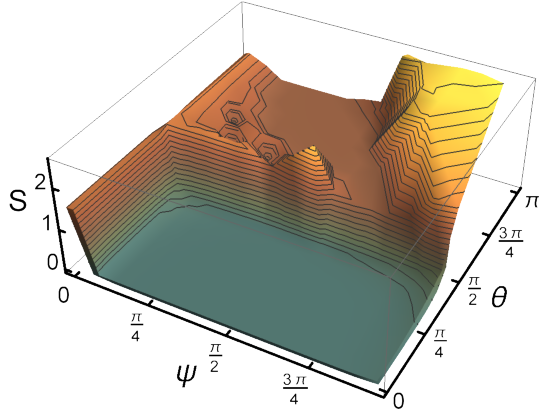
\includegraphics[width=0.8\textwidth]{data/Plots/Plot19.pdf}\\
	\vspace{20pt}
	\begin{tikzpicture}
	\node at (0,0) {(\textbf{b)}};
	\end{tikzpicture}\\
	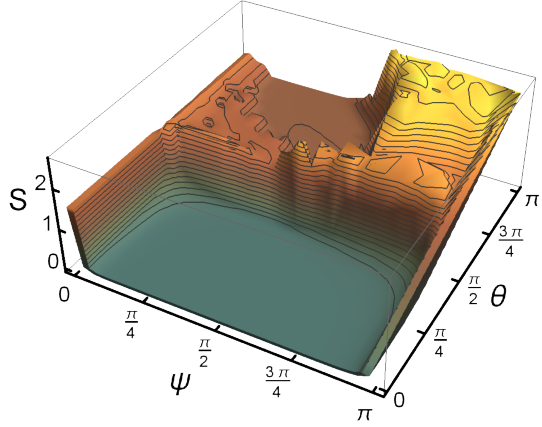
\includegraphics[width=0.8\textwidth]{data/3Dplot19.pdf}
	\caption{\small \label{fig:fullent}\textbf{Entropy landscape for }$\varphi=\frac{19\pi}{16}$: \textbf{(a)} Coarse diagram: $\psi,\theta\in[0,\pi]$, where the interval is split into $16$ pieces. Here, we observe an isolated peak in the middle of the diagram. \textbf{(b)} Finer diagram: The interval $[0,\pi]$ is split into $32$ pieces. The isolated peak is split into several smaller peaks.}
\end{figure}
%\newpage

In \cref{fig:fullent} the entropy landscape for $\varphi=\frac{19\pi}{16}$ is shown. The upper plot in \cref{fig:fullent}\textbf{(a)} shows the coarse overview, while the lower plot in \cref{fig:fullent}\textbf{(b)} gives a finer landscape where the interval $[0,\pi]$ is split into $32$ pieces instead of $16$. In general, there seem to be roughly three different regions in this landscape: There is one big region (green) where the entropy stays zero regardless of the bond dimension. This region exists in all plots in \cref{app:H3chain} for $\theta\in[0,\frac{\pi}{2}]$ (roughly), regardless of the values of $\varphi$ and $\psi$. Another region, depicted in brown, has a value of $S\approx 1$, and the third region (yellow) consists of points with $S\approx 2$. This is consistent with the two-dimensional entropy landscape depicted in \cref{fig:Ent1rho}. Hence, candidates for critical points are at the borders between these regions. In the coarse overview we are looking for points where the entanglement entropy decreases, as explained above. In most of the plots the transition between the regions does not show an unusual high value for the entropy. 

In one of the plots, which is shown in \cref{fig:fullent}\textbf{(a)}, we observe a rather isolated peak at the boarder of the $S\approx 0$ and the $S\approx 1$ region, hence we take a closer look at this plot. In \cref{fig:fullent}\textbf{(b)}, a finer version of the landscape is shown where we have collected more data points. Here, it becomes clear that the emergence of the isolated peak was merely due to the small number of data points than a reflection of the physical behaviour of the system. Furthermore, a more detailed analysis of the scaling of the entanglement entropy shows that it saturates instead of diverging with growing bond dimension.

In the end, we have not been able to identify any critical points for the anyon chain built from the fusion category $\Hd$.


\section{Further directions}

We conclude from our numerical investigation of anyon chains built from the fusion category $\Hd$ that the system does not show critical behaviour, hence it does not correspond to a conformal field theory. However, this does not mean that there is no conformal field theory associated to the Haagerup subfactor. It is merely an indicator that building the anyon chain directly from the fusion category instead of a modular category is the wrong approach to the problem. A more promising yet also more complicated idea is to start from the quantum double of the fusion category $\Hd$ (which is indeed a unitary modular tensor category) and study the corresponding anyon chain. 

Before following this approach, for completeness we can also check whether the other two categories in the Morita equivalence class, $\Hi_1$ and $\Hi_2$, yields a CFT via the anyon chain construction. Even though we do not expect a positive result here, these calculations are still easier to do than going via the quantum double. Furthermore, since the fusion rules of the category $\Hi_1$ contain multiplicities (which is also the case for the quantum double of these categories), this construction can be helpful to understand the additional challenges that come with multiplicities in anyon chains. In contrast to the quantum double, which has twelve simple objects, $\Hi_1$ only has four simples and is therefore easier to handle.

The approach that uses the UMTC, however, brings new challenges: First, we have to construct the quantum double of the fusion category $\Hd$\footnote{We could also use $\Hi_1$ or $\Hi_2$, for that matter, since they are Morita equivalent and therefore yield the same quantum double.}. Some work has already been done in this direction, for instance the simple objects have been identified and the modular data has been constructed (see \cite{izumi_structure_2001,SEUNGMOON2008,Evans2011,Grossman2015}). However, an important ingredient in the construction of an anyon chain Hamiltonian are the $F$-symbols of the category, which have not yet been determined for the quantum double of the Haagerup subfactor. Hence, before we can numerically investigate the anyon chain that corresponds to the quantum double, we have to find its $F$-symbols. Since the category includes twelve simple objects and, moreover, has fusion rules with multiplicities, finding the $F$-symbols is a much more challenging task than it was for the $\Hd$ category.
